%\chapter[ความพื้นฐานเกี่ยวกับยูนิกซ์และลินุกซ์]{\makebox[\headwidth][r]{\sffamily\bfseries ความรู้เบื้องต้นเกี่ยวกับยูนิกซ์และลินุกซ์}}\label{chap:basic}
\begin{thwbr}
%\chapter{ความรู้พื้นฐานเกี่ยวกับลินุกซ์}\label{chap:basic}
\chapter{ลินุกซ์ขั้นพื้นฐาน}\label{chap:basic}

\begin{flushright}
{\it\latintext ``LINUX is obsolete''}\\
{\bf\latintext Andrew Tanenbaum }
\end{flushright}

%ในบทนี้จะเป็นการแนะนำความรู้เบื้องต้นก่อนที่จะเริ่มใช้ลินุกซ์. 
%จากที่ได้แนะนำไปแล้วว่าลินุกซ์เป็นระบบปฏิบัติการคล้ายเหมือนระบบปฏิบัติการยูนิกซ์, ประกอบด้วยเคอร์เนลและประแกรมใช้งานต่างๆให้เป็นระบบ. 

จากบทที่ \ref{chap:intro} เราได้ทราบแล้วว่าลินุกซ์สร้างขึ้นมาโดยมียูนิกซ์เป็นต้นแบบ. คำจำกัดความอย่างง่ายๆและสั้นๆของลินุกซ์ในช่วงที่เกิดใหม่ๆคือ ``unix clone''. กล่าวคือลินุกซ์ทำอะไรได้ทุกอย่างที่ยูนิกซ์ทำได้. เมื่อวันเวลาผ่านไป, ลินุกซ์พัฒนาไปเรื่อยๆเพิ่มความสามารถคุณสมบัติพิเศษต่างๆจนไม่อาจจะเรียกว่าเป็น unix clone ได้อีกต่อไป. อย่างไรก็ตามคำสั่งหรือโปรแกรมพื้นฐานต่างๆที่ใช้ในยูนิกซ์ได้ก็จะมีอยู่ในลินุกซ์ด้วย. บางโปรแกรมอาจจะทำงานเหมือนกันทุกประการ, บางโปรแกรมที่มีชื่อเหมือนกันอาจจะทำงานต่างกัน, หรือบางโปรแกรมที่ยูนิกซ์ไม่มีแต่ลินุกซ์มี.

ในบทนี้จะแนะนำความรู้พื้นฐานเกี่ยวกับลินุกซ์ซึ่งจะครอบคลุมถึงยูนิกซ์บางส่วนด้วย. เนื้อหาส่วนใหญ่จะเกี่ยวกับการใช้งาน\emph{เชลล์ (shell)}\myvocab{s}{shell}{\emph{เชลล์}. โปรแกรมที่เป็นตัวกลางระหว่างผู้ใช้กับเคอร์เนล. มีหน้าที่แปลคำสั่งจากคีย์บอร์ดส่งต่อให้เคอร์เนลทำงานที่ต้องการ. เชลล์ที่นิยมใช้กับลินุกซ์ได้แก่ \cmd{bash}, \cmd{csh}, \cmd{ksh}, \cmd{zsh} เป็นต้น.} และจะแทรกตัวอย่างการใช้โปรแกรมต่างๆด้วย. นอกจากนั้นจะแนะนำความรู้เบื้องต้นทั่วๆไปที่เกี่ยวกับตัวระบบปฏิบัติการเองด้วย.

ผู้อ่านจะทำความเข้าใจตัวอย่างได้ง่ายขึ้นถ้าติดตั้งลินุกซ์ไว้เรียบร้อยแล้วและทดลองตามไปด้วย. ลินุกซ์ที่ติดตั้งจะเป็นดิสทริบิวชันค่ายใดก็ได้แล้วแต่สะดวก. ผู้อ่านสามารถอ่านรายละเอียดการติดตั้งลินุกซ์ได้จากภาคผนวก. 

\section{ระบบปฏิบัติการ}
เนื่องจากลินุกซ์เป็นระบบปฏิบัติการ, จึงมีความสำคัญอย่างยิ่งที่ผู้อ่านควรจะทำความเข้าใจว่าระบบปฏิบัติการคืออะไรและมีการทำงานอย่างไร. เมื่อผู้อ่านมีความรู้เบื้องต้นเกี่ยวกับระบบปฏิบัติการแล้วก็จะทำให้ผู้อ่านเข้าใจการทำงานของลินุกซ์และใช้งานลินุกซ์ได้ดีขึ้นด้วย.

สำหรับความหมายทั่วไป, ลินุกซ์หมายถึงตัวระบบปฏิบัติการซึ่งได้เคอร์เนลและโปรแกรมต่างๆประกอบขึ้นเป็นระบบที่ใช้งานกับคอมพิวเตอร์. เพื่อความชัดเจนยิ่งขึ้น, ต่อไปนี้จะใช้คำว่า ``ลินุกซ์'' ในความหมายทั่วไปและจะใช้คำว่า ``ลินุกซ์เคอร์เนล'' เจาะจงถึงตัวเคอร์เนลซึ่งเป็นหัวใจของระบบปฏิบัติการ. 

\begin{figure}
\plfigure{.4}{os.eps}{ความสัมพันธ์ระหว่างระบบปฏิบัติการ, ฮาร์ดแวร์และซอฟต์แวร์}{os}
\end{figure}

รูปที่%
\myvocab{i}{interface}{\emph{อินเทอร์เฟส}. หมายถึงตัวเชื่อมหรือตัวกลางระหว่างของสองสิ่ง. ตัวอย่างเช่น เชลล์เป็นอินเทอร์เฟสแบบคำสั่งบรรทัดระหว่างยูสเซอร์กับเคอร์เนล. X วินโดว์เป็นอินเทอร์เฟสแบบหน้าต่างใช้เมาส์และคีย์บอร์ดในการป้อนข้อมูล}\myvocab{p}{program}{\emph{โปรแกรม}. ชุดคำสั่งภาษาเครื่องกล (machine language) ที่สามารถโหลดเข้าไปในหน่วยความจำและหน่วยประมวลผลแปลความภาษาเครื่องกลเพื่อที่จะทำงานต่อไป.}\myvocab{f}{file}{\emph{ไฟล์}, \emph{แฟ้มข้อมูล}. ไฟล์คือข้อมูลซึ่งอาจจะเก็บบันทึกในหน่วยความจำถาวรเช่นฮาร์ดดิกส์เป็นต้น. ข้อมูลที่เรียกว่าไฟล์นี้มีลำดับ, ข้อมูลที่บันทึกก่อนจะอยู่ในช่วงต้นของไฟล์. ข้อมูลที่เก็บล่าสุดจะอยู่ในช่วงท้ายของไฟล์.}%
 \ref{fig:os} แสดงภาพรวมของระบบคอมพิวเตอร์โดยทั่วไป. คอมพิวเตอร์ (ฮาร์ดแวร์) ไม่สามารถทำงานได้ถ้าไม่มีระบบปฏิบัติการ (ซอฟต์แวร์). ผู้ใช้ไม่สามารถใช้คอมพิวเตอร์ได้ถ้าไม่มีโปรแกรมหรือซอฟต์แวร์ต่างๆเป็น\emph{ตัวกลาง (interface)} ระหว่างผู้ใช้กับระบบปฏิบัติการ. เคอร์เนลเป็นซอฟต์แวร์พิเศษที่ควบคุมการทำงานของฮาร์ดแวร์ต่างๆที่ประกอบกันเป็นคอมพิวเตอร์. ผู้ใช้ไม่สามารถติดต่อใช้งานเคอร์เนลได้โดยตรง, ต้องสั่งงานที่ต้องการทำผ่านทางเชลล์, X วินโดว์ หรือโปรแกรมอื่นๆ. ในรูปที่ \ref{fig:os} มีการแยกเชลล์, X วินโดว์ และโปรแกรมอื่นๆออกจากกัน. แต่ถ้ามองจากจุดยืนของเคอร์เนลแล้ว, เชลล์หรือ X วินโดว์เป็นเพียงสิ่งที่เรียกว่า\emph{โปรแกรม (program)} เท่านั้น, ไม่มีความแตกต่างกันแต่ประการใด. โปรแกรมเหล่านี้เรียกอีกอย่างได้ว่าเป็น\emph{ซอฟต์แวร์อินเทอร์เฟส (software interface)} ให้กับเคอร์เนล. 

%\begin{figure}[!htb]
%\plfigure{.4}{program_process.eps}{โปรแกรมและโปรเซส}{program_process}
%\end{figure}


โปรแกรมคือ\emph{ไฟล์ (file)} %
ข้อมูลที่บันทึกคำสั่งเป็น\emph{ภาษาเครื่องกล (machine language)}%
\myvocab{m}{machine language}{\emph{ภาษาเครื่องกล}. ข้อมูลที่หน่วยประมวลผลเข้าใจและแปลความหมายเพื่อทำงานได้.} %
เก็บไว้ในหน่วยความจำถาวรเช่นฮาร์ดดิกส์. เมื่อสั่งคำสั่งเรียกใช้โปรแกรมแล้ว, เคอร์เนลจะอ่านเนื้อหาของไฟล์ (โปรแกรม) แล้ว\emph{โหลด (load)} บันทึกในหน่วยความจำ. เคอร์เนลจะควบคุมให้หน่วยประมวลผลอ่านข้อมูลที่อยู่บนหน่วยความจำกระทำการต่างๆต่อไป. โปรแกรมที่โหลดขึ้นสู่หน่วยความจำและกำลังทำงานอยู่เรียกว่า\emph{โปรเซส (process)}.%
\myvocab{p}{process}{\emph{โปรเซส}. สภาพที่โปรแกรมที่กำลังทำงานอยู่. กล่าวคือเนื้อหาของตัวโปรแกรมถูกโหลดจากฮาร์ดดิกส์ไปที่หน่วยความจำและหน่วยประมวลผลข้อมูลแปลคำสั่งเพื่อที่จะกระทำการต่อไป.}



ลินุกซ์เคอร์เนลสร้างขึ้นมาด้วย\emph{ภาษาซี (C language)} %
กับ\emph{ภาษาแอสเซมบลี (assembly language)} %
บางส่วน. การที่โปรแกรมและ\emph{ไลบรารี (library)} ต่างๆจะติดต่อกับเคอร์เนลเพื่อสั่งงาน, ต้องติดต่อผ่านทาง\emph{ซิสเตมคอล (system call)} ซึ่งเป็น\emph{ฟังชัน (function)} ในภาษาซี.

\section{การเข้าสู่ระบบ}
ลินุกซ์เป็นระบบปฏิบัติการที่\emph{ผู้ใช้ (user)} หลายคนสามารถใช้งานได้ในเวลาเดียวกัน. ผู้ใช้แต่ละคนจะมี\emph{ชื่อล็อกอิน (login name)} และ\emph{รหัสผ่าน (password)}\mymemo{การเข้าสู่ระบบของระบบปฏิบัติการ Windows จะเรียกว่า logon แต่สำหรับโลกของยูนิกซ์จะเรียกว่า login}
เฉพาะที่แตกต่างกัน. ผู้ใช้ต้อง\emph{ล็อกอิน (login)}
เข้าสู่ระบบเพื่อที่จะใช้คอมพิวเตอร์ผ่านทางเชลล์หรือ X วินโดว์ต่อไป. 

ผู้ใช้ที่มีอำนาจสูงสุดในระบบได้แก่ \emph{root} ทำหน้าที่ดูแลระบบเช่น สร้างผู้ใช้ทั่วไป, ติดตั้งโปรแกรมลงในระบบ, ปรับแต่งระบบ เป็นต้น. ตอนติดตั้งลินุกซ์, โปรแกรมติดตั้งจะสร้างผู้ใช้ที่เป็น root ให้โดยปริยายแล้วให้สร้างรหัสผ่านด้วย. โดยทั่วๆไป, โปรแกรมติดตั้งจะเปิดโอกาสให้สร้างผู้ใช้อื่นๆด้วย. เนื่องจาก root สามารถทำอะไรก็ได้กับระบบเช่นลบไฟล์อะไรก็ได้, จึงทำให้การล็อกอินเป็น root ไม่ปลอดภัยเท่าที่ควรเพราะอาจเผลอเรอลบไฟล์ที่จำเป็นกับระบบปฏิบัติการทิ้งไปโดยไม่ตั้งใจ. ดังนั้นจึงไม่ควรล็อกอินเป็น root ถ้าไม่จำเป็น.
\myvocab{c}{C language}{\emph{ภาษาซี}. ภาษาคอมพิวเตอร์ที่มนุษย์สามารถอ่านทำความเข้าใจได้. เป็นภาษาชั้นสูงที่มีไวยกรณ์แน่นอน. โดยปรกติผู้ใช้จะคอมไพล์รหัสต้นฉบับที่เขียนด้วยภาษาซีเพื่อแปลงเป็นภาษาเครื่องกลที่คอมพิวเตอร์เข้าใจซึ่งเรียกว่าโปรแกรม. ภาษาซีสร้างโดย Dennis Ritchie นักวิจัยของ Bell Laboratories ในราวปี ค.ศ. 1972. ภาษาซีเป็นภาษาใช้งานทั่วไป (general purpose) และใช้ในสร้างระบบปฏิบัติการยูนิกซ์ในเวลาต่อมา. ลินุกซ์เคอร์เนลและโปรแกรมใช้งานส่วนใหญ่ก็ใช้ภาษาซีเขียนเช่นกัน.}\myvocab{a}{assembly language}{\emph{ภาษาแอสเซมบลี}. ภาษาคอมพิวเตอร์ชั้นต่ำ, มีความขึ้นอยู่กับสถาปัตยกรรมที่ใช้มากทำให้ยากต่อการพอร์ตโปรแกรมไปใช้กับสถาปัตยกรรมอื่นๆ.}%
%
\subsection{ผู้ใช้ในระบบ}
ผู้ใช้ในระบบปฏิบัติการลินุกซ์และยูนิกซ์จะมีหมายเลขประจำตัวซึ่งเรียกว่า \emph{user ID}\gindex{user ID} หรือเรียกย่อๆว่า \emph{UID}\gindex{uid@UID} เป็นหมายเลขเฉพาะสำหรับเคอร์เนลไว้แยกแยะผู้ใช้แต่ละคน. ผู้ใช้แต่ละคนจะอยู่ใน\emph{กรุป (group)}\gindex{group}\gindex{กรุป} ที่กำหนดไว้อย่างน้อยหนึ่งกลุ่ม. เคอร์เนลจะแยกแยะกรุปของผู้ใช้ด้วยหมายเลขเฉพาะเรียกว่า \emph{group ID}\gindex{group ID} หรือเรียกย่อๆว่า \emph{GID}\gindex{gid@GID}. ผู้ใช้จะมีสิทธิ์การใช้คำสั่ง, หรือการใช้ไฟล์ต่างๆกันขึ้นอยู่กับกรุปที่ตัวเองอยู่และ UID. 

ในระบบปฏิบัติการลินุกซ์จะมีผู้ใช้ที่ระบบเตรียมอยู่ไว้แล้วเช่น bin, daemon ฯลฯ. ผู้เหล่านี้บางรายไม่ได้มีตัวตนจริง, ระบบจะใช้ผู้ใช้เหล่านี้ในการรันโปรแกรมพิเศษต่างๆเช่นโปรแกรมเซิฟร์เวอร์เป็นต้น. ในระบบยังมีกลุ่มที่เตรียมไว้อยู่แล้วเช่นเดียวกับผู้ใช้เช่น bin, wheel, sys, mail ฯลฯ. ผู้ใช้ที่อยู่ในกลุ่ม mail ก็จะได้รับอนุญาตให้กระทำการต่างๆที่เกี่ยวกับการดูและระบบ mail ได้เป็นต้น.

วิธีการสำรวจ UID และ GID จะใช้คำสั่ง \cmd{id}\cindex{id}\refcmd{id} ซึ่งจะแสดง UID และ GID ของผู้ใช้ที่สั่งคำสั่งนั้น.
\begin{MyExample}[สำรวจ UID และ GID.]
\begin{MyEx}
$ \cin{id}
uid=1000(poonlap) gid=100(users) groups=10(wheel),18(audio),100(users)
\end{MyEx}
\end{MyExample}%$


ในระบบปฏิบัติการลินุกซ์จะมีโปรแกรม ``\cmd{su}'' %
\refcmd{su}%
 สำหรับเปลี่ยน UID ของผู้ใช้ให้เป็น UID ของคนอื่น. เช่นใช้เปลี่ยนผู้ใช้ที่ล็อกอินอยู่เป็น root.\mymemo{เครื่องหมาย \cmd{\cursorprompt} แสดงถึงคีย์บอร์ด\emph{เคอร์เซอร์ (cursor)}}

\cindex{su}%
\begin{MyExample}[การใช้ \cmd{su} ด้วยตัวเลือก \cmd{-}]
\begin{MyEx}
$ \cin{su -}
Password: \mycomment{รหัสผ่านที่พิมพ์จะไม่แสดงบนหน้าจอ}
# \cursorprompt \mycomment{ล็อกอินเชลล์ของ root ซึ่งอ่านค่าเริ่มต้นต่างๆแล้ว}
\end{MyEx}
\end{MyExample}%$
จากตัวอย่างเป็นการใช้คำสั่ง \cmd{su} กับ\emph{ตัวเลือก (option)} ``\cmd{-}'' หมายถึงการเปลี่ยนผู้ใช้เป็น root และใช้ล็อกอินเชลล์. การใช้ตัวเลือก \cmd{-} จะเป็นการบอกให้เชลล์อ่านค่าติดตั้งเริ่มต้นของ root. ถ้าไม่ต้องการให้เชลล์อ่านค่าติดตั้งเริ่มต้นของ root ให้สั่งคำสั่ง \cmd{su} โดยไม่มีตัวเลือก.
\begin{MyExample}[การใช้คำสั่ง \cmd{su} ไม่มีตัวเลือก]
\begin{MyEx}
$ \cin{su}
Password: \mycomment{รหัสผ่านที่พิมพ์จะไม่แสดงบนหน้าจอ}
# \cursorprompt \mycomment{เชลล์เชิงโต้ตอบ, ไม่มีการอ่านค่าเริ่มต้นของ root}
\end{MyEx}
\end{MyExample}%$

คำสั่งที่คล้ายกับคำสั่ง \cmd{su} คือ \cmd{sg}\cindex{sg}\refcmd{sg} ซึ่งเป็นคำสั่งเปลี่ยนกลุ่มหลักเป็นกลุ่มอื่น.
\begin{MyExample}[การเปลี่ยนกลุ่ม.]
\begin{MyEx}
$ \cin{sg wheel}
$ \cin{id}
uid=1000(poonlap) gid=10(wheel) groups=10(wheel),18(audio),27(video),100(users)
\end{MyEx}
\end{MyExample}
จากตัวอย่างจะเห็นว่ากลุ่มปัจจุบันหรือกลุ่มปัจจุบันเปลี่ยนเป็น wheel แทนกลุ่มโดยปริยาย users. นอกจากคำสั่ง \cmd{sg} แล้วยังมีคำสั่ง \cmd{newgrp}\cindex{newgrp}\refcmd{newgrp} ซึ่งทำหน้าที่คล้ายกับ \cmd{sg}.

UID และ GID นี่จะเกี่ยวข้องกับสิทธิ์การใช้ไฟล์, รันโปรแกรม ซึ่งจะแนะนำในบทถัดไป.

\subsection{ประเภทของการล็อกอินแบ่งตามอินเทอร์เฟส}
\subsubsection{เท็กซ์โหมด (text mode)}%
\myvocab{t}{text mode}{\emph{เท็กซ์โหมด}. สภาพของระบบปฏิบัติที่อินเทอร์เฟสเป็นคีย์บอร์ดและหน้าจอเทอร์มินัลเท่านั้น.}%
\mymemo{ในเท็กซ์โหมด, ถ้าผู้ใช้ธรรมดากดคีย์ \ovalbox{\cmd{Ctrl}}+\ovalbox{\cmd{Alt}}+\ovalbox{\cmd{Del}} จะทำให้ลินุกซ์\emph{รีบูต (reboot)}. ผู้ดูแลระบบสามารถปรับแต่งระบบได้ถ้าไม่ต้องการให้ผู้ใช้รีบูตเครื่องได้ด้วยวิธีนี้}%
ตัวอย่างต่อไปนี้แสดงตัวอย่างการล็อกอินของผู้ใช้ชื่อ somchai แบบ\emph{เท็กซ์โหมด (text mode)} ผ่านทางเทอร์มินอล. การล็อกอินในลักษณะนี้มักจะเป็นการล็อกอินจาก\emph{คอนโซล (console)} หรือใช้คำสั่ง \cmd{telnet}%
%\refcmd{telnet}
%\myexplanation{telnet [\textit{hostname}]}{user interface to the \underline{TELNET} protocol. โปรแกรมสื่อสารใช้เข้าสู่ระบบเครื่องคอมพิวเตอร์ที่ต้องการที่โดยผ่านทางเน็ตเวิร์ก.\\
%\cmdit{hostname}: ชื่อเครื่องที่อยู่บนเน็ตเวิร์กหรือ IP address.} %
ล็อกอินผ่านทางเน็ตเวิร์กจากคอมพิวเตอร์เครื่องอื่น.


\begin{MyExample}[การล็อกอินแบบเท็กซ์โหมด]\label{ex:prompt}
\begin{MyEx}
login: \cin{somchai}
Password: \mycomment{รหัสผ่านที่พิมพ์จะไม่แสดงบนหน้าจอ}
[somchai@toybox somchai]$ \cursorprompt
\end{MyEx}
\end{MyExample}%$

เมื่อล็อกอินแล้วผู้ใช้สามารถสั่งคำสั่งต่างๆได้โดยการพิมพ์คำสั่งจากคีย์บอร์ด. อินเทอร์เฟสแบบนี้เรียกกันว่า \underline{C}ommand \underline{L}ine \underline{I}nterface (CLI)\gindex{cli@CLI|see{Command Line Interface}}\gindex{command line interface@Command Line Interface} หรืแ \underline{T}ext \underline{U}ser \underline{I}nterface \gindex{tui@TUI|see{Text User Interface}}\gindex{text user interface@Text User Interface}.%
\myvocab{c}{command line interface}{ระบบอินเทอร์เฟสที่ใช้คีย์บอร์ดและหน้าจอแสดงตัวอักษรเป็นหลัก. ถ้าเป็นงานที่ไม่ต้องการกราฟฟิกจะเป็นอินเทอร์เฟสที่สะดวกมากและปฏิบัติการได้เร็วกว่า graphical user interface.} เราเรียก ``\cmd{[somchai@toybox somchai]\char36}'' ว่า\emph{เชลล์พรอมต์ (shell prompt)} %
\myvocab{p}{prompt}{\emph{พรอมต์}. เครื่องหมาย, หรืออักษรที่เชลล์แสดงทางหน้าจอเพื่อแสดงว่าพร้อมที่จะรับคำสั่งจากคีย์บอร์ด.}%
บ่งบอกว่าเชลล์พร้อมที่จะรับคำสั่งจากคีย์บอร์ด. 

ตัวอย่างที่ \ref{ex:prompt} แสดงเป็นพรอมต์ที่ปรับแต่งให้จากดิสทริบิวชันโดยแสดงชื่อผู้ใช้ (somchai), ชื่อโฮส (toybox) และชื่อไดเรกทอรีปัจจุบัน (somchai). เชลล์ที่ทำงานหน้าที่รอรับคำสั่งหลังจากการล็อกอินเรียกว่า\emph{ล็อกอินเชลล์ (login shell)}. ส่วนเชลล์ที่ไม่ใช่ล็อกอินเชลล์เราเรียกว่า\emph{เชลล์เชิงโต้ตอบ (interactive shell)}. เชลล์เชิงโต้ตอบเป็นเชลล์ที่ไม่ได้เกิดจากการล็อกอินแต่เป็นการเรียกโปรแกรมเชลล์มาใช้งานเฉยๆ, เช่นการใช้เชลล์ในเทอร์มินอลเอมิวเลเตอร์. เชลล์จะทำงานอยู่ในไดเรกทอรีที่เรียกว่า\emph{โฮมไดเรกทอรี (home directory)} %
\myvocab{h}{home directory}{\emph{โฮมไดเรกทอรี}. ไดเรกทอรีที่ผู้ใช้เป็นเจ้าของ. เป็นไดเรกทอรีเริ่มต้นเวลาล็อกอินเข้าสู่ระบบหรือเรียกใช้เทอร์มินัลเอมิวเลเตอร์.}%
ซึ่งเป็นไดเรกทอรีเริ่มต้นหลังจากการล็อกอิน. ไดเรกทอรีนี้เป็นพื้นที่เฉพาะของผู้ใช้ที่ล็อกอินสำหรับเก็บข้อมูลต่างๆ. ผู้ใช้มีสิทธิ์ที่จะสร้างไฟล์หรือสร้างไดเรกทอรีเพิ่มเติมในโฮมไดเรกทอรีของตัวเอง.\mymemo{ในโลกของ Windows จะเรียกไดเรกทอรีว่าโฟลเดอร์ (folder)}

ล็อกอินเชลล์และเชลล์โต้ตอบต่างกันที่เวลาเริ่มต้นการทำงาน, ล็อกอินเชลล์จะอ่านและเซ็ตค่าเริ่มต้นการทำงานเช่นค่าตัวแปรสภาพแวดล้อมจากไฟล์ \cmd{/etc/profile} ถ้ามีไฟล์นี้อยู่ในระบบ. หลังจากนั้นจะหาไฟล์ \cmd{.bash\_profile}, \cmd{.bash\_login} และ \cmd{.login} ที่อยู่ในโฮมไดเรกทอรีตามลำดับ. ถ้าเจอไฟล์ไหนก่อนก็จะอ่านค่าเริ่มต้นจากไฟล์นั้น. ส่วนเชลล์เชิงโต้ตอบจะอ่านค่าเริ่มต้นจากไฟล์ \cmd{.bashrc} ที่อยู่ในโฮมไดเรกทอรีเท่านั้น. 
\myvocab{g}{graphic mode}{\emph{กราฟฟิกโหมด}. สภาพที่ระบบปฏิบัติการใช้อินเทอร์เฟสแบบกราฟฟิกติดต่อกับผู้ใช้. โดยทั่วไปคอมพิวเตอร์แบบกราฟฟิกโหมดสามารถผลเป็นแบบหน้าต่าง, สร้างปุ่ม, เมนู ฯลฯ. ผู้ใช้โต้ตอบกับคอมพิวเตอร์ด้วยคีย์บอร์ดและเมาส์.}%
\myvocab{x}{X Display Manager}{หน้าจอแบบกราฟฟิกใช้ในการล็อกอิน. ก่อนที่จะมี GNOME และ KDE, ระบบ X วินโดว์ใช้ X Display Manager ที่เรียกว่า \cmd{xdm} ซึ่งปัจจุบันไม่นิยมใช้กันแล้ว. โปรแกรมที่มาแทน \cmd{xdm} ได้แก่ \cmd{gdm}, \cmd{kdm} ฯลฯ.}%
\myvocab{x}{X server}{\emph{X เซิร์ฟเวอร์}. โปรแกรมแบบ server - client ที่มีหน้าที่รับคำขอจาก client วาดหน้าจอ, ผลิตหน้าต่าง, ควบคุมระบบหน้าต่าง ฯลฯ.}%



เพื่อความสะดวกในการอ่าน, ต่อจากนี้เป็นต้นไปจะใช้เครื่องหมาย ``\cmd{\char36}'' แทนเชลล์พรอมต์ของผู้ใช้ธรรมดา. 
\begin{MyExample}[เชลล์พรอมต์ของผู้ใช้ทั่วไป]
\begin{MyEx}
$ \cursorprompt
\end{MyEx}
\end{MyExample}
และใช้เครื่องหมาย ``\cmd{\#}'' แทนเชลล์พรอมต์ของ root.
\begin{MyExample}[เชลล์พรอมต์ของ root]
\begin{MyEx}
# \cursorprompt
\end{MyEx}
\end{MyExample}%$



\subsubsection{กราฟฟิกโหมด (graphic mode)}%
\mymemo{ในกราฟฟิกโหมด, ถ้าผู้ใช้กดคีย์ \ovalbox{\cmd{Ctrl}}+\ovalbox{\cmd{Alt}}+\ovalbox{\cmd{BackSpace}} จะเป็นการยกเลิกการทำงาน X เซิร์ฟเวอร์ที่ใช้อยู่. ผู้ดูแลระบบสามารถปรับแต่งระบบให้ยกเลิกการใช้คีย์เหล่านี้ได้.}%
รูปที่ \ref{fig:gdm} แสดงตัวอย่างหน้าจอล็อกอินแบบ\emph{กราฟฟิกโหมด (graphic mode)}. หน้าจอล็อกอินเป็นโปรแกรมที่เรียกว่า X Display Manager %
มีหน้าที่ถามชื่อผู้ใช้และรหัสผ่าน. โปรแกรมหน้าจอต้อนรับเข้าสู่ระบบนี้มีหลายประเภทเช่น \cmd{xdm}, \cmd{gdm}, \cmd{kdm} เป็นต้น. %\myxapp{xdm, gdm, kdm}{Display Manager, โปรแกรมหน้าจอต้อนรับเข้าสู่ระบบ}
การล็อกอินแบบนี้ต้องการคอมพิวเตอร์ที่สามารถแสดงผลแบบกราฟฟิกทางหน้าจอได้.

\begin{figure}[!tb]
\plfigure{.35}{gdm.eps}{หน้าจอล็อกอินแบบกราฟฟิก}{gdm}
%\scalebox{.35}{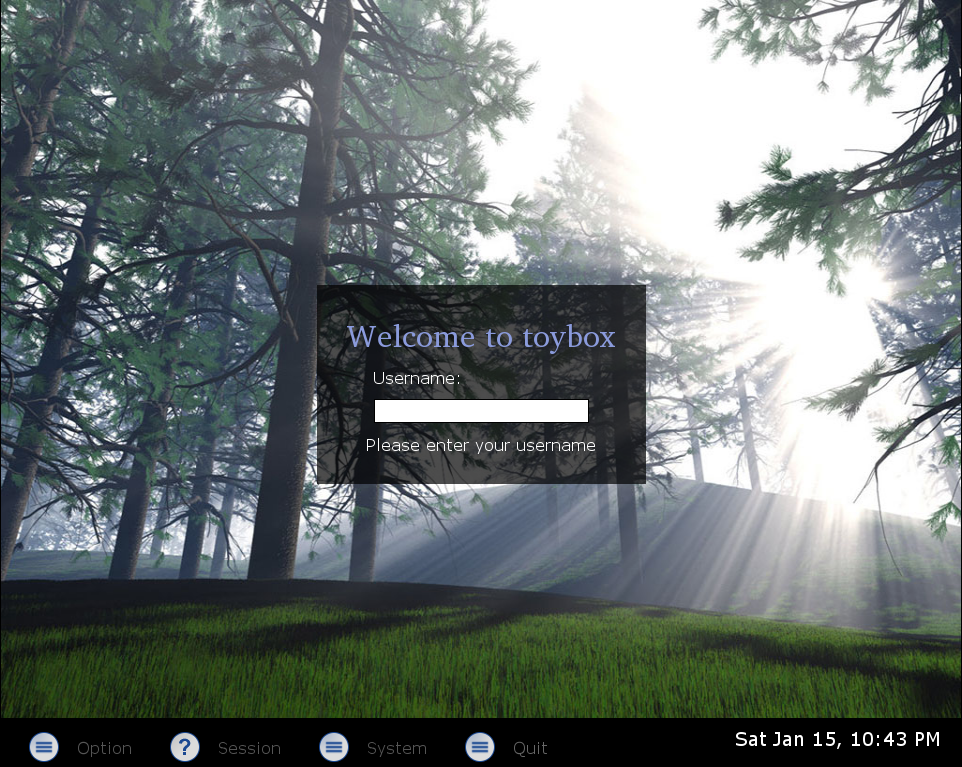
\includegraphics{gdm.eps}}
%\caption{หน้าจอล็อกอินแบบกราฟฟิก}\label{fig:gdm}
\end{figure}

%\marginpar{\scalebox{.2}{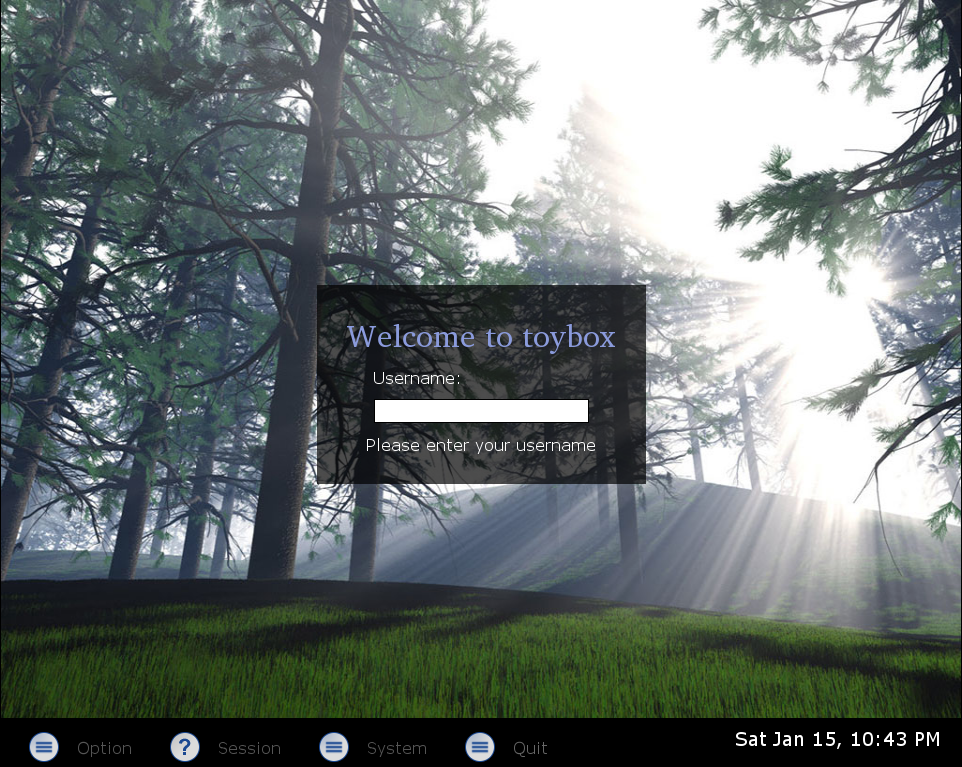
\includegraphics{gdm.eps}}}

กราฟฟิกโหมดต่างจากเท็กซ์โหมดตรงที่มี \emph{X เซิร์ฟเวอร์ (X server)} %
ซึ่งเป็นโปรแกรมพื้นฐานสำหรับระบบวินโดว์คอยรับคำสั่งสร้างส่วนประกอบของกราฟฟิก. ดิสทริบิวชันทั่วไปมักจะมีระบบ Desktop Environment %
เช่น GNOME หรือ KDE เป็นระบบเดกส์ท็อปมาตรฐานให้ผู้ใช้ใช้งาน. ระบบ desktop environment \myvocab{d}{Desktop Environment}{ระบบ, สภาพแวดล้อมที่เสนอกราฟฟิกอินเทอร์เฟสสำหรับผู้ใช้โดยที่อินเทอร์เฟสเหล่านั้นมีความเข้ากันได้ดีเช่นรูปร่างหน้าตาเหมือนหรือคล้ายกัน, ทำงานร่วมกันได้ ฯลฯ. ตัวอย่าง Desktop Environment ที่นิยมได้แก่ GNOME, KDE เป็นต้น.}%
นี้เองที่เป็นตัวจัดการการทุกอย่างที่เกี่ยวกับเดกส์ท็อปเช่นหน้าจอล็อกอิน, เมนู, โปรแกรมสำหรับใช้งานที่เป็นแบบ graphical user interface (GUI) %
\myvocab{g}{graphical user interface (GUI)}{อินเทอร์เฟสแบบกราฟฟิกที่แสดงหน้าต่าง, ปุ่มกด, เมนู ทางหน้าจอ. ผู้ใช้จะใช้เมาส์หรือคีย์บอร์ดในการโต้ตอบกันระบบ.}%
ให้. ในกราฟฟิกโหมดผู้ใช้จะใช้งานได้สะดวกกว่าเท็กซ์โหมด, เพราะสามารถรันโปรแกรมหลายโปรแกรมโดยที่แต่ละโปรแกรมมีวินโดว์เฉพาะของตัวเอง. เนื่องจากระบบ GUI มีเมนูต่างๆเตรียมไว้ให้, ผู้ใช้ที่ไม่คุ้นเคยกับการใช้เชลล์ก็สามารถใช้โปรแกรมต่างๆได้สะดวกขึ้น.

ในระบบ X วินโดว์, ผู้ใช้จะใช้เชลล์ผ่านทาง\emph{เทอร์มินอลเอมิวเลเตอร์ (terminal emulator)} %
\myvocab{t}{terminal emulator}{\emph{เทอร์มินอลเอมิวเลเตอร์}. โปรแกรมที่จำลองหน้าจอแสดงผลตัวอักษรเพื่อใช้กับเชลล์. เทอร์มินอลเอมิวเลเตอร์จะเป็นโปรแกรมที่ใช้ใน X วินโดว์เช่น \cmd{xterm}, \cmd{gnome-terminal}, \cmd{konsole} เป็นต้น.}%
ซึ่งเป็นโปรแกรม GUI ที่จำลองจอภาพเพื่อแสดงผลบนระบบ X วินโดว์. โปรแกรมเทอร์มินอลเอมิวเลเตอร์มีหลายปรเภทเช่น \cmd{xterm}, \cmd{gnome-terminal}, \cmd{konsole} ขึ้นอยู่กับความชอบพอของผู้ใช้. โปรแกรมเหล่านี้จะเตรียมเชลล์เชิงโต้ตอบซึ่งจะรอแปรคำสั่งที่ป้อนเข้ามาทางคีย์บอร์ดต่อไป.


\begin{figure}[!tb]
\plfigure{.5}{sample_terminal.eps}{เทอร์มินอลเอมูเลเตอร์ (\cmd{gnome-terminal}) ที่รันบน X วินโดว์}{terminalemu}
\end{figure}

อินเทอร์เฟสแบบ CLI และ GUI มีจุดเด่นและจุดด้อยแตกต่างกันไป. ผู้ใช้ไม่ต้องใช้เชลล์เลยก็ได้ถ้าล็อกอินเข้าทางกราฟฟิกโหมด. GUI สะดวกในการใช้เพราะเราเห็นทุกอย่างเป็นสิ่งที่จับต้องได้เช่นหน้าต่างๆ, ปุ่ม, เมนู. ในทางกลับกันข้อดีนี้ก็อาจจะกลายเป็นข้อด้อยได้เช่นกัน. เช่นเมนูของการกระทำที่โปรแกรมเตรียมไว้ไม่เพียงพอ, คอมพิวเตอร์ที่ใช้ไม่มีประสิทธิภาพเพียงพอที่จะรันโปรแกรมให้เร็ว, ไม่สามารถทำงานที่ต้องการโดยอัตโนมัติได้เพราะผู้ใช้ต้องโต้ตอบกับโปรแกรมนั้นๆเสมอ. ข้อโดยที่ยกตัวอย่างไปนี้เป็นสิ่งที่เชลล์ถนัด. กล่าวคือเชลล์มีไม่ยึดติดกับงานอย่างใดอย่างหนึ่ง, เราสามารถใช้คำสั่งบรรทัดหลายๆคำสั่งรวมกันทำงานเฉพาะที่เราต้องการได้. ที่สำคัญคือเชลล์ทำงานได้ทั้งแบบเชิงโต้ตอบและแบบอัติโนมัติ. ถ้าเรารู้สิ่งขั้นตอนของงานที่เราต้องการทำก็สามารถเขียน\emph{เชลล์สคริปต์ (shell script)} %
\myvocab{s}{shell script}{\emph{เชลล์สคริปต์}. ไฟล์ที่รวมคำสั่งที่ใช้ในเชลล์เข้าด้วยกัน. เชลล์จะตีความคำสั่งที่อยู่ในไฟล์นั้นบรรทัดต่อบรรทัด. สะดวกสำหรับการสั่งคำที่เป็นขั้นตอน. เนื่องจากเชลล์มีไวยกรณ์, สามารถสร้างตัวแปร, สามารถควบคุมข้อแม้ต่างๆได้จึงถือเป็นภาษาคอมพิวเตอร์แบบ interpreter ด้วย. เชลล์สคริปต์มีบทบาทสำคัญกับลินุกซ์มากเช่น เชลล์สคริปต์ใช้ในการเริ่มต้นโปรแกรมเซิร์ฟเวอร์ต่างๆ.}%
ให้ทำงานโดยอัตโนมัติได้. ส่วนข้อด้อยของเชลล์คือไม่สะดวกในการใช้สำหรับผู้ที่ไม่คุ้นเคย. \mymemo{ที่ผมใช้คำว่า ``ไม่สะดวกในการใช้สำหรับผู้ที่ไม่คุ้นเคย'' แทนคำว่า ``ไม่สะดวกในการใช้'' เพราะเป็นความจริงที่ว่าความยากง่ายของการใช้อยู่ที่ความเคยชิน} และงานในหลายอย่างต้องการการสิ่งที่นอกเหนือจาก\emph{ข้อมูลเท็กซ์ (text data)} %
\myvocab{t}{text data}{\emph{ข้อมูลเท็กซ์}. ข้อมูลที่หรือไฟล์ที่มนุษย์สามารถอ่านแล้วเข้าใจได้. โดยปรกติข้อมูลเท็กซ์จะหมายถึงไฟล์ที่เขียนด้วยภาษาอังกฤษที่อ่านได้, ไม่มีอักขระควบคุม (control character) ปะปน.}%
เช่นการตัดต่อวีดีโอ, การดูข้อมูลทางเว็บ เป็นต้น. 


\subsection{การล็อกอินแบ่งตามการใช้เน็ตเวิร์ก}
\subsubsection{ล็อกอินผ่านคอนโซล}
\emph{คอนโซล (console)} หมายถึงชุดคีย์บอร์ดและจอแสดงผลที่ต่อโดยตรงกับคอมพิวเตอร์. การล็อกอินผ่านทางคอนโซลเป็นการล็อกอินแบบไม่ใช้เน็ตเวิร์ก, จะเป็นการล็อกอินแบบเท็กซ์โหมดหรือกราฟฟิกโหมดก็ได้แล้วแต่ความสามารถของคอมพิวเตอร์ในการแสดงผล.
\subsubsection{ล็อกอินผ่านทางเน็ตเวิร์ก}
การล็อกอินประเภทผ่านทางเน็ตเวิร์กทำได้โดยใช้โปรแกรมเช่น \cmd{telnet}, \cmd{ssh}, \cmd{X} ฯลฯ ติดต่อกับเครื่องคอมพิวเตอร์ที่ต้องการล็อกอิน. การล็อกอินผ่านทางเน็ตเวิร์กสามารทำได้ทั้งแบบเท็กซ์โหมดและกราฟฟิกโหมดโดยใช้\emph{เน็ตเวิร์กโปรโตคอล (network protocol)} ที่แตกต่างกัน. ตัวอย่างเช่นโปรแกรม \cmd{telnet} จะใช้โปรโตคอล telnet ในการสื่อสารระหว่างคอมพิวเตอร์, การล็อกอินแบบกราฟฟิกจะใช้โปรโตคอล xdmcp (X Disaplay Manager Control Protocol) เป็นต้น. 


\section{การออกจากระบบ}
\subsection{เท็กซ์โหมด}
เมื่อต้องการออกจากระบบให้ใช้คำสั่ง ``\cmd{logout}''.\mymemo{การออกจากระบบของระบบปฏิบัติการ Windows เรียกว่า logoff แต่ในโลกของยูนิกซ์จะเรียกว่า logout}\refcmd{logout}


\cindex{logout}%
\begin{MyExample}[การล็อกเอาท์แบบเท็กซ์โหมด]
\begin{MyEx}
$ \cin{logout}
\arrowdown \thtt{ระบบจะเคลียร์หน้าจอและรอการล็อกอินต่อไป}
login: \cursorprompt
\end{MyEx}
\end{MyExample}%$


คำสั่ง \cmd{logout} นี้จะทำได้เมื่อล็อกอินเท่านั้น. เพราะว่าเชลล์ของเทอร์มินอลเอมูลเตอร์ไม่ใช่ล็อกอินเชลล์จึงใช้คำสั่ง \cmd{logout} ไม่ได้, ให้ใช้คำสั่ง ``\cmd{exit}'' แทน.\refcmd{exit}
\cindex{exit} สิ่งที่แตกต่างกันระหว่าง \cmd{logout} กับ \cmd{exit} คือ \cmd{logout} จะอ่านคำสั่งหรือค่าติดตั้งในไฟล์ \cmd{.bash\_logout} ที่อยู่ในโฮมไดเรกทอรีก่อนจะจบการทำงานของเชลล์. ส่วนคำสั่ง \cmd{exit} จะจบการทำงานของเชลล์เฉยๆ. โดยทั่วไปแล้วการกดคีย์ \ovalbox{\cmd{Ctrl}}+\ovalbox{\cmd{d}} ในเชลล์พรอมต์ก็เป็นการจบการทำงานของเชลล์ได้เช่นกัน. \mymemo{\ovalbox{\cmd{Ctrl}}+\ovalbox{\cmd{d}} เป็นอักขระควบคุมเทอร์มินอลหมายถึงไม่มีข้อมูลนำเข้าอีกต่อไป (end of file). ซึ่งก็หมายถึงการจบการทำงานของเชลล์.} 



\subsection{กราฟฟิกโหมด}
ในระบบ Desktop Environment จะมีเมนูหลักสำหรับให้ผู้ใช้เลือกเพื่อล็อกเอาท์ออกจากระบบ.


\section{เทอร์มินอลเสมือน}
โดยปรกติคอมพิวเตอร์หนึ่งเครื่องจะมีคอนโซลหนึ่งชุด. เมื่อผู้ใช้คนหนึ่งล็อกอินผ่านทางคอนโซล, ผู้ใช้คนอื่นจะไม่สามารถใช้คอมพิวเตอร์ได้จนกว่าผู้ใช้ที่ใช้คอนโซลล็อกเอาท์. ถ้าต้องการล็อกอินเข้าสู่ระบบเดียวกันพร้อมๆกัน, ผู้ใช้คนอื่นต้องล็อกอินผ่านทางเน็ตเวิร์ก. ลินุกซ์คอนโซลสามารถแก้ปัญหานี้ได้ด้วยสิ่งที่เรียกว่า\emph{เทอร์มินอลเสมือน (virtual terminal)}. %
\myvocab{v}{virtual terminal}{\emph{เทอร์มินอลเสมือน}. เทอร์มินอลในเท็กซ์โหมดของลินุกซ์ที่สามารถเปลี่ยนหน้าจอเป็นหลายหน้าจอได้โดยมีหน้าจอที่เป็นรูปธรรมเพียงหน้าจอเดียว. วิธีเปลี่ยนหน้าจอทำได้โดยกด \ovalbox{\cmd{Ctrl}} และ \ovalbox{\cmd{Alt}} ร่วมกับฟังก์ชันคีย์.}%
เทอร์มินอลเสมือนจะจำลองคอนโซลให้มีหลายชุดในเวลาเดียวกัน. อย่างไรก็ตามเนื่องจากคอมพิวเตอร์หนึ่งเครื่องจะมีคีย์บอร์ด, เมาส์และจอแสดงผลเพียงหนึ่งชุดเท่านั้น, เวลาเปลี่ยนคอนโซลโดยใช้เทอร์มินอลเสมือนจะใช้การกดคีย์ \ovalbox{\cmd{Ctrl}} และ \ovalbox{\cmd{Alt}} ร่วมกับ\emph{ฟั่งชันคีย์ (function key)}. 

\begin{figure}[!htb]
\plfigure{.45}{virtual_terminal.eps}{เทอร์มินอลเสมือน}{virtual_terminal}
\end{figure}

\subsection{การเปลี่ยนโหมด}
สมมติว่าผู้อ่านกำลังล็อกอินด้วยกราฟฟิกโหมดอยู่และต้องการเปลี่ยนเป็นเท็กซ์โหมด, ผู้อ่านสามารถทำได้โดยกดคีย์ \ovalbox{\cmd{Ctrl}}+\ovalbox{\cmd{Alt}}+\ovalbox{\cmd{F1}}\mymemo{\ovalbox{\cmd{Ctrl}}+\ovalbox{\cmd{Alt}}+\ovalbox{\cmd{F1}} หมายความว่าให้กดคีย์ \ovalbox{\cmd{Ctrl}} และ \ovalbox{\cmd{Alt}} ค้างไว้แล้วกดคีย์ \ovalbox{\cmd{F1}} ตาม. ในเท็กซ์โหมดไม่ต้องกดคีย์ \ovalbox{\cmd{Ctrl}} ก็ให้ผลเหมือนกัน.} เพื่อเปลียนเป็นเทอร์มินัลที่ 1 (ดูรูปที่ \ref{fig:virtual_terminal} ประกอบ). กดคีย์ \ovalbox{\cmd{Ctrl}}+\ovalbox{\cmd{Alt}}+\ovalbox{\cmd{F2}} เพื่อเปลี่ยนเป็นเทอร์มินัลที่ 2 ซึ่งเป็นเท็กซ์โหมดเช่นกัน. ถ้าจะเปลี่ยนกลับเป็นกราฟฟิกโหมดเหมือนเดิมให้กดคีย์ \ovalbox{\cmd{Ctrl}}+\ovalbox{\cmd{Alt}}+\ovalbox{\cmd{F7}}. 

โดยปรกติแล้ว X เซิร์ฟเวอร์จะรันอยู่ตัวเดียวเพราะฉะนั้นเทอร์มินอลที่เป็นกราฟฟิกโหมดจะเป็นเทอร์มินอลที่ 7 (\cmd{F7}) เท่านั้น. ถ้ามี X เซิร์ฟเวอร์รันอยู่มากกว่าหนึ่งตัว, X เซิร์ฟเวอร์ตัวที่สองจะรันอยู่ที่คอนโซลที่ 8 (\cmd{F8}) เป็นต้น.

ตัวอย่างการใช้เทอร์มินอลเสมือนเช่น นาย ก. ใช้คอมพิวเตอร์รันโปรแกรมคำนวณซึ่งกินเวลาเป็นชั่วโมงอยู่และล็อกอินค้างไว้. นาย ข. มีธุระด่วนต้องอ่านเมลล์และไม่มีคอมพิวเตอร์ตัวอื่นให้ล็อกอินผ่านทางเน็ตเวิอร์ก. ถ้าเป็นคอมพิวเตอร์ที่ไม่ใช่ลินุกซ์ นาย ก. ต้องล็อกเอาท์เพื่อให้นาย ข. ใช้คอมพิวเตอร์. ในกรณีนี้นาย ก. ไม่จำเป็นต้องล็อกเอาท์ออกจากระบบ, เพียงแต่เปลียนเป็นเทอร์มินัลเสมือนเป็นตัวอื่นให้นาย ข. ได้ใช้ชั่วคราวโดยที่ไม่มีผลกระทบกับโปรแกรมที่ตัวเองรันอยู่. เมื่อนาย ข. ใช้งานเสร็จก็เปลี่ยนเทอร์มินัลเสมือนกลับเป็นตัวเดิมให้นาย ก. ใช้อีกที. ตัวอย่างการใช้เทอร์มินอลเสมือนอื่นๆเช่น การเปลี่ยนจากกราฟฟิกโหมดเป็นเท็กซ์โหมดเวลากราฟฟิกโหมดมีปัญหาไม่สามารถรับข้อมูลจากคีย์บอร์ดหรือเมาส์ได้. 

\section{เชลล์เบื้องต้น}\mymemo{หลายคนเข้าใจผิดว่าเชลล์คือหรือเหมือน DOS (Disk Operating System). ในความเป็นจริงแล้ว DOS คือระบบปฏิบัติการแต่เชลล์คือโปรแกรม. แต่ทั้งเชลล์และ DOS ใช้อินเทอร์เฟส CLI จึงทำให้คนทั่วไปคิดว่าเชลล์และ DOS เหมือนกัน.}
ในปัจจุบันถึงแม้ว่าอินเทอร์เฟสแบบกราฟฟิกจะเป็นที่นิยมกันอย่างกว้างขวางแต่ไม่ได้หมายความว่าอินเทอร์เฟสแบบบรรทัดคำสั่งเป็นสิ่งล้าสมัย. เชลล์เป็นโปรแกรมแอินเทอร์เฟสที่โต้ตอบกับผู้ใช้คอมพิวเตอร์โดยอาศัยแป้นพิมพ์และการแสดงผลเป็นตัวอักษรเป็นหลัก. เนื่องจากความต้องการพื้นฐานของเชลล์ได้แก่แป้นพิมพ์และจอภาพที่สามารถแสดงตัวอักษร, ทำให้คอมพิวเตอร์ที่ใช้ไม่จำเป็นต้องมีทรัพยากรมากก็ใช้ได้. การแสดงผลเป็นตัวอักษร, ข้อความซึ่งเป็นภาษาที่มนุษย์เข้าใจได้ทันที. สำหรับผู้ที่คุ้นเคยกับแป้นพิมพ์สามารถสั่งคำสั่งได้รวดเร็วเมื่อเปรียบเทียบกับการใช้เมาส์. %
\mymemo{การใช้เมาส์ถือว่าช้ากว่าการใช้แป้นพิมพ์เพราะผู้ใช้ต้องกระทำการหลายขั้นตอนได้แก่ เลื่อนเมาส์, เล็งจุดของเมาส์ให้ตรงกับตำแหน่งที่ต้องการ, กดเมาส์, เลือกเมนู ฯลฯ. ถ้าผู้ใช้วางตำแหน่งนิ้วได้ถูกต้องและจำตำแหน่งของคีย์ต่างๆได้จะเร็วมาก. ถ้าเทียบเวลาการเรียนรู้แล้ว, เมาส์ใช้เวลาเรียนรู้น้อยกว่าการเรียนใช้แป้นพิมพ์.}
และที่สำคัญที่สุดคือผู้ใช้สามารถเขียนคำสั่งเป็นขั้นตอนแล้วดำเนินการทีเดียวได้แบบอัตโนมัติ. ด้วยเหตุผลเหล่านี้เองที่ผู้ใช้ใหม่ควรจะศึกษาการใช้เชลล์อย่างจริงจังเพื่อที่จะเป็นพื้นฐานในการใช้ลินุกซ์ต่อไป. 

ในระบบปฏิบัติการยูนิกซ์ยุคแรกใช้เชลล์ที่เรียกกันว่า Bourne shell (\cmd{sh})\mymemo{ในระบบลินุกซ์ \cmd{sh} จะเป็น symbolic link ของ \cmd{bash}.} ซึ่งตั้งชื่อตามผู้สร้างคือนาย Stephen Bourne. หลังจากที่เกิด BSD ยูนิกซ์, Bill Joy ได้สร้างเชลล์ที่มีไวร์กรณ์คล้ายกับภาษาซีและมีความสามารถพิเศษมากขึ้นกว่าเดิมเรียกว่า C shell (\cmd{csh}). นอกจากนี้ยังมีเชลล์หลายตัวเกิดขึ้นเช่น Korn shell (\cmd{ksh}), Bourne-again shell (\cmd{bash}), Zsh (\cmd{zsh})\mymemo{``z'' ใน zsh มีความหมายแฝงหมายถึงเชลล์ตัวสุดท้าย. zsh เป็นเชลล์ที่รวบรวมสิ่งดีๆของเชลล์ต่างๆรวมกันและมีจุดมุ่งหมายเป็นเชลล์ที่ดีที่สุดในบรรดาเชลล์ทั้งหลาย.} ฯลฯ. ในระบบปฏิบัติการลินุกซ์เลือกใช้ Bourne-again shell, หรือที่เรียกสั้นๆว่า \cmd{bash} เป็นเชลล์ปริยาย. Bash เป็นโปรแกรมหนึ่งในโปรเจค GNU. Bash สร้างขึ้นโดย Brain Fox และ Chet Ramey ให้มีความเข้ากันได้กับ Bourne เชลล์มีจุดเด่นในการแก้ไขบรรทัดคำสั่ง, การโต้ตอบกับผู้ใช้, การเติมเต็มคำสั่งหรือไฟล์ ฯลฯ.

สำหรับระบบปฏิบัติการตระกูลยูนิกซ์, ผู้ใช้นิยมที่จะสั่งคำสั่งให้คอมพิวเตอร์หรือเคอร์เนลทำงานโดยผ่านเชลล์. สาเหตุที่เรียกว่าเชลล์เพราะเชลล์ทำหน้าที่เป็นเปลือกหุ้มเป็นตัวกลางระหว่างเคอร์เนลและผู้ใช้. ในทางทฤษฎี, เชลล์เป็น\emph{โปรแกรมแปรคำสั่ง (command interpreter)} อย่างหนึ่งที่มีคุณสมบัติ\emph{เชิงโต้ตอบ (interactive)} กับผู้ใช้, มีความสามารถควบคุมการดำเนินงาน, รับตัวแปรซึ่งอาจจะเป็นค่าที่พิมพ์จากคีย์บอร์ดหรือชื่อไฟล์ส่งต่อให้โปรแกรม, เรียกกระทำการโปรแกรมต่างๆ, รับและส่งข้อมูลให้กับโปรแกรมที่เรียกใช้เป็นต้น. 

\emph{คำสั่ง (command)} %
\myvocab{c}{command}{\emph{คำสั่ง}. คำหรือตัวอักษรที่พิมพ์ทางแป้นพิมพ์ส่งต่อให้เชลล์แปลความหมายและกระทำการต่อไป. ความหมายทั่วไปยังหมายถึงโปรแกรมหรือชื่อโปรแกรมที่เรียกใช้ผ่านเชลล์.}
ที่เชลล์แปรความในที่นี้อาจจะหมายถึงคำสั่งที่เชลล์สามารถกระทำการเองได้ซึ่งเรียกว่า\emph{คำสั่งภายใน (shell built-in command)} %
\mymemo{ตัวอย่างคำสั่งภายในเช่น \cmd{cd}, \cmd{pwd}, \cmd{fg} เป็นต้น. ตัวอย่างคำสั่งภายนอกหรือโปรแกรมได้แก่คำสั่ง \cmd{ls}, \cmd{cp}, \cmd{rm} ฯลฯ.}%
หรือคำสั่งที่เชลล์ไม่สามารถกระทำการได้เองเรียกว่า\emph{คำสั่งภายนอก (external shell command)} ซึ่งก็คือ\emph{โปรแกรม (program)} นั่นเอง. 

\subsection{อักขระ}
อักขระ (character) \mymemo{อักขระหมายถึงตัวอักษรรวมถึงเครื่องหมายต่างๆ.}ที่พิมพ์ในเชลล์พรอมต์โดยปรกติได้แก่อักษรภาษาอังกฤษที่เรียกว่าอักขระ ASCII (American Standard Code for Information Interchange) ซึ่งแสดงในตารางที่ \ref{tab:ascii} (หน้า \pageref{tab:ascii}). อักขระ ASCII ยังแบ่งได้เป็น\emph{อักขระควบคุม (control character)}\mymemo{เนื่องจากอักขระควบคุมเหล่านี้ไม่มีรูปร่างหน้าตา, บางครั้งจึงเรียกว่า non-printable character.} สำหรับควบคุมการประมวลผลข้อมูลหรือควบคุมการส่งข้อมูล, และ\emph{อักขระกราฟฟิก (graphic character)} ซึ่งเป็นอักขระที่พิมพ์แล้วมองเห็นได้ซึ่งได้แก่อักษรภาษาอังกฤษรวมถึงเครื่องหมายต่างๆที่ใช้ทั่วไป.

%แบ่งออกเป็นสองประเภทคืออักขระที่แสดงทางหน้าจอได้ (printable character) กับอักขระที่ไม่สามารถแสดงทางหน้าจอได้ (non-printable character). อักขระที่แสดงทางหน้าจอได้ได้แก่อักขระที่พิมพ์จากคีย์บอร์ดแล้วสามารถเห็นสิ่งที่พิมพ์ไปเช่นเมื่อกดคีย์ \ovalbox{\texttt{a}} ก็จะปรากฎตัวอักษร ``a'' ทางหน้าจอ. ส่วนอักขระที่ไม่สามารถแสดงทางหน้าจอได้เช่นเมื่อกดคีย์ \ovalbox{\texttt{Enter}} จะเป็นการสั่งให้เชลล์แปลคำสั่งที่พิมพ์ไป. อักขระที่ใช้ในเชลล์เหล่านี้โดยทั่วไปได้แก่


%อักขระที่ไม่สามารถแสดงทางหน้าจอได้มีชื่อเรียกอีกอย่างว่า\emph{อักขระควบคุม (control character)} . ตัวอย่างเช่นเราสามารถกดคีย์ \ovalbox{\texttt{BackSpace}} เพื่อลบอักขระที่พิมพ์ไปแล้ว. การกดคีย์ \ovalbox{\texttt{BackSpace}} จริงๆแล้วเป็นการส่งอักขระ BS ซึ่งเป็นอักขระควบคุมข้อมูลที่ส่งไปแล้ว. จากตาราง \ref{tab:ascii} (หน้า \pageref{tab:ascii}) จะเห็นว่าเราไม่สามารถพิมพ์อักขระทั้งหมดได้ด้วยคีย์บอร์ด. คีย์บอร์ดส่วมมากจะมีคีย์สำหรับอักขระควบคุมที่ใช้บ่อยเท่านั้นเช่น \kk{BackSpace}, \kk{Delete}, \kk{Tab}, \kk{Enter} เป็นต้น. ในกรณีที่คีย์บอร์ดไม่มีคีย์เหล่านี้, ผู้ใช้สามารถกดคีย์ C-h แทน \ovalbox{\texttt{BackSpace}}, C-m แทน \ovalbox{\texttt{Enter}} ได้. นอกจากนี้ถ้ากด C-d (EOT) เชลล์จะถือว่าไม่มีข้อมูลนำเข้าแล้วจะจบการทำงานโดยปริยาย. การใช้ C-h, C-m, C-d นี้เป็นการตีความของอักขระในระดับเทอร์มินอล. กล่าวคือเมื่อเรากด C-h แล้วเทอร์มินอลจะแปลงเป็นอักขระ BS ส่งให้เชลล์ต่อไป. 



โดยทั่วไป, ผู้ใช้สามารถพิมพ์อักขระกราฟฟิกได้ด้วยคีย์บอร์ด. แต่อักขระควบคุมที่ใช้บ่อยบางตัวเท่านั้นที่สามารถพิมพ์จากคีย์บอร์ดได้โดยตรงเช่น \kk{Backspace} \kk{Tab} \kk{Enter} เป็นต้น. ในกรณีที่คีย์บอร์ดที่ใช้ไม่มีคีย์พิเศษดังกล่าว, เราสามารถกดปุ่ม \kk{Ctrl} ค้างไว้แล้วกดคีย์ตัวอักษรภาษาอังกฤษตามเพื่อสร้างอักขระควบคุมได้. ตัวอย่างเช่น \kk{Ctrl}+\kk{h} ใช้แทน \kk{Backspace}, \kk{Ctrl}+\kk{i} ใช้แทน \kk{Tab} และ \kk{Ctrl}+\kk{m} ใช้แทน \kk{Enter} เป็นต้น.


อักขระควบคุมบางตัวมีความหมายพิเศษต่อเทอร์มินอลหรือเชลล์. ตัวอย่างเช่นอักขระ EOT (\underline{E}nd \underline{O}f \underline{T}ransmission) %
\mymemo{บ้างก็เรียก EOT ว่า EOF (\underline{E}nd \underline{O}f \underline{F}ile).}%
หมายถึงสิ้นสุดข้อมูลนำเข้า. ผู้ใช้สามารถส่งอักขระควบคุมนี้โดยกดคีย์ \kk{Ctrl}+\kk{d} ในเชลล์พรอมต์เพื่อจบการทำงานของเชลล์. การกดคีย์ \kk{Ctrl}+\kk{l} จะหมายถึง FF (\underline{F}orm \underline{F}eed) ซึ่งมีความหมายถึงการขึ้นหน้าใหม่. ในกรณีนี้สิ่งที่แสดงบนหน้าจอไปแล้วจะถูกลบทิ้ง (เคลียร์) แล้วจะเหลือเชลล์พรอมต์ไว้ที่บรรทัดเริ่มต้น. ตารางที่ \ref{tab:controlterm} แสดงอักขระควบคุมที่ใช้บ่อย. 

\bigskip
\tablecaption{อักขระควบคุมที่มีความหมายพิเศษต่อเทอร์มินอลหรือเชลล์}\label{tab:controlterm}
\tablefirsthead{\hline \multicolumn{1}{c|}{อักขระควบคุม} & \multicolumn{1}{|c|}{คีย์} & \multicolumn{1}{|c}{คำอธิบาย}\\
\hline
}
\tablehead{\multicolumn{3}{l}{{\slshape ต่อจากหน้าที่แล้ว}}\\ \hline \multicolumn{1}{c|}{อักขระควบคุม} & \multicolumn{1}{|c|}{คีย์} & \multicolumn{1}{|c}{คำอธิบาย}\\
\hline
}
\tabletail{\hline \multicolumn{3}{r}{\slshape ต่อหน้าถัดไป}\\}
\tablelasttail{\hline}
\begin{supertabular}{c|c|p{.5\textwidth}}
%SOH & \kk{Ctrl}+\kk{a}  & เลื่อนเคอร์เซอร์ไปที่ต้นบรรทัด, ใช้แทน \Ovalbox{Home} ได้\\
%SOT & \kk{Ctrl}+\kk{b}  & เลื่อนเคอร์เซอร์ถอยหลังหนึ่งตัวอักขระ, ใช้แทน \kk{\myleftarrow} ได้\\ 
ETX & \kk{Ctrl}+\kk{c} & สัญญาณ SIGINT (interrupt) ยกเลิกการทำงานของคำสั่ง\\
EOT & \kk{Ctrl}+\kk{d} & สิ้นสุดข้อมูลนำเข้า, จบการทำงานในกรณีที่ใช้อักขระควบคุมนี้เป็นตัวแรกในเชลล์พรอมต์\\
 &  & ลบตัวอักษรที่อยู่ตรงเคอร์เซอร์ในกรณีที่พิมพ์คำสั่งอยู่, ใช้แทน \Ovalbox{Del} ได้\\
%ENQ & \kk{Ctrl}+\kk{e}& เลื่อนเคอร์เซอร์ไปที่ท้ายบรรทัด, ใช้แทน \Ovalbox{End} ได้\\
%ACK & \kk{Ctrl}+\kk{f} & เลื่อนเคอร์เซอร์ไปข้างหน้าหนึ่งตัวอักขระ, ใช้แทน \kk{\arrowright} ได้\\
%BEL & \kk{Ctrl}+\kk{g} & กระดิ่งหรือยกเลิกการจัดแต่บรรทัด\\
%BS & \kk{Ctrl}+\kk{h} & ลบอักขระที่อยู่หน้าเคอร์เซอร์หนึ่งตัว, ใช้แทน \Ovalbox{Backspace} ได้\\
%VT & \kk{Ctrl}+\kk{k} & ลบอักขระตั้งแต่เคอร์เซอร์ไปจนสุดบรรทัด\\
%FF & \kk{Ctrl}+\kk{l} & เคลียร์หน้าจอ\\
%CR & \kk{Ctrl}+\kk{m} & จบบรรทัด, ใช้แทน \Ovalbox{Enter} หรือ \Ovalbox{Return} ได้\\
%SO & \kk{Ctrl}+\kk{n} หรือ \kk{arrowdown} & ประวัติคำสั่งถัดไป\\
%DLE & \kk{Ctrl}+\kk{p} หรือ \kk{arrowup} & ประวัติคำสั่งก่อนหน้านี้\\
DC1 & \kk{Ctrl}+\kk{q} & แสดงผลทางหน้าจออีกครั้งหลังจากที่ถูกหยุดด้วยอักขระควบคุม DC3 \\
%DC2 & \kk{Ctrl}+\kk{r} & ค้นหาประวัติคำสั่งย้อนหลัง\\
DC3 & \kk{Ctrl}+\kk{s} & หยุดการแสดงผลทางหน้าจอชั่วคราว (ขึ้นอยู่กับเทอร์มินอลที่ใช้)\\
SUB & \kk{Ctrl}+\kk{z} & สัญญาณ SIGSTOP (stop) หยุดการทำงานของคำสั่ง(ชั่วคราว)\\
\end{supertabular}
\bigskip





%ในการทำงานระดับเชลล์เราสามารถแบ่งประเภทของอักขระได้ดังนี้.
%
%\begin{itemize}
%\item blank: ได้แก่ SP และ TAB ใช้เป็นตัวแบ่งระหว่างคำ.
%\item control operator: ได้แก่ CR, NL, ``||'', ``\&\&'', ``\&'', ``;'', ``;;'', ``|'', ``(``, และ ``)'' เป็นตัวอักขระควบคุมการดำเนินคำสั่งของเชลล์. 
%\item metacharacter: ได้แก่ blank หรือ ``|'', ``\&'', ``;'', ``(``, ``)'', ``<'', ``>'' ถือเป็นตัวแบ่งคำเมื่อไม่ได้ quote. \mymemo{การ quote หมายถึงการใช้เครื่องหมาย double quote หรือ single quote กำกับ.}
%\item wildcard: ใช้ในการระบุชื่อไฟล์, ได้แก่เครื่องหมาย ``*'' แทนอักษรใดๆตั้งแต่ศูนย์ตัวขึ้นไป. เครื่องหมาย ``?'' แทนอักษรใดๆก็ได้หนึ่งตัวเท่านั้น. เมื่อเครื่องหมาย ``*'' หรือ ``?'' อยู่ใน quote เชลล์จะไม่ตีความเป็น wildcard.
%
%
%\item escape: ได้แก่ ``\bs'' ใช้พิมพ์นำหน้าอักขระพิเศษเพื่อไม่ให้เชลล์ตีความหมายแบบอักขระเหล่านั้น, ให้ถือเป็นอักขระธรรมดา. ตัวอย่างเช่น
%\end{itemize}


\subsection{คำสั่ง}
คำสั่งคือสิ่งที่ต้องการให้คอมพิวเตอร์ทำงาน. ถ้าคอมพิวเตอร์เข้าใจภาษามนุษย์, เราอาจจะสั่งคำสั่งได้ดังต่อไปนี้.

\begin{MyVerbatim}
{\thaitext\it ในสภาพแวดล้อมที่กำหนด} {\thaitext\it ให้ทำสิ่งที่สั่ง(ทำอะไร)} {\thaitext\it แบบนี้(ทำอย่างไร)} {\thaitext\it โดยให้ใช้ข้อมูลต่อไปนี้}
\end{MyVerbatim}

การสั่งคำสั่งในเชลล์พรอมต์ก็มีลักษณะคล้ายกับการสั่งคำสั่งด้วยวาจาโดยมีรูปแบบการสั่งคำสั่งทั่วไปเป็น\mymemo{เครื่องหมาย \myenter{} ใช้แสดงถึงการกดคีย์ \kk{Enter} และเครื่องหมาย \cmd{\char32} แสดงถึงช่องไฟ.}

%\begin{figure}[!htb]
%\caption{รูปแบบการสั่งคำสั่ง}
%\begin{MyVerbatim}
%{\thaitext\textbf{แบบง่าย:}}
%$ {\thaitext\textbf{คำสั่ง}}\char32{\thaitext\textit{อาร์กิวเมนต์}}\char32{\thaitext\textit{อาร์กิวเมนต์}}\char32... \myenter
%{\thaitext\textbf{แบบทั่วไป:}}
%$ {\thaitext\textit{ตัวแปรสภาพแวดล้อม=ค่า}}\char32{\thaitext\textit{ตัวแปรสภาพแวดล้อม=ค่า}}\char32...\char32{\thaitext\textbf{คำสั่ง}}\char32{\thaitext\textit{อาร์กิวเมนต์}}\char32{\thaitext\textit{อาร์กิวเมนต์}}\char32... \myenter
%\end{MyVerbatim}
%\end{figure}


\begin{MyVerbatim}
$ {\thaitext\textit{ตัวแปรสภาพแวดล้อม=ค่า}}\char32{\thaitext\textit{ตัวแปรสภาพแวดล้อม=ค่า}}\char32...\char32{\thaitext\textbf{คำสั่ง}}\char32{\thaitext\textit{อาร์กิวเมนต์}}\char32{\thaitext\textit{อาร์กิวเมนต์}}\char32... \myenter
\end{MyVerbatim}

ส่วนที่จำเป็นในการสั่งคำสั่งได้แก่ชื่อคำสั่ง. ส่วนที่เป็น ``\textit{ตัวแปรสภาพแวดล้อม=ค่า}'' และ ``\textit{อาร์กิวเมนต์}'' จะมีหรือไม่มีก็ได้. 

คำสั่งโดยปรกติจะเป็น ``คำ'' ภาษาอังกฤษ. คำในที่นี้หมายถึงการนำอักษรภาษาอังกฤษมาเรียงกันซึ่งอาจจะไม่มีความหมายก็ได้. คำในที่นี้ยังหมายถึงกลุ่มอักษรที่แบ่งได้ด้วยช่องไฟหรือแคร่เช่น \cmd{abc def} จะถือว่ามีสองคำคือ \cmd{abc} กับ \cmd{def}. เชลล์ยังแยกแยะความแตกต่างระหว่างตัวอักษรภาษาอังกฤษตัวเล็ก (small letter) และตัวใหญ่ (capital letter) ด้วย.\mymemo{ชื่ออีกแบบของตัวอักษรภาษาอังกฤษตัวเล็กคือ lower-case letter. และชื่อของตัวอักษรภาษาอังกฤษตัวใหญ่คือ upper-case letter.}

เมื่อผู้ใช้กดคีย์ \Ovalbox{\cmd{Enter}} แล้ว, เชลล์จะตรวจสอบว่าคำที่ใส่เข้าไปนั้นเป็นอะไร, ถ้าเชลล์สามารถตีความได้ก็จะทำงานตามที่สั่งต่อไป. เมื่องานที่สั่งไปจบเรียบร้อยแล้วเชลล์ก็จะแสดงเชลล์พรอมต์เพื่อที่จะรับคำสั่งถัดไปเรื่อยๆเป็นวัฐจักรตามรูปที่ \ref{fig:shell_circle}.

\begin{figure}[!htb]
\plfigure{.5}{shell_circle.eps}{วงจรการรันคำสั่งของเชลล์}{shell_circle}
\end{figure}

สิ่งที่อยู่หน้าคำสั่ง (มีหรือไม่ก็ได้) ได้แก่\emph{ตัวแปรสภาพแวดล้อม (environment variable)} และค่าของตัวแปรนั้นๆ. ให้สังเกตว่าตัวแปรและค่าของตัวแปรขั้นด้วยเครื่องหมายเท่ากับโดยที่ข้างหน้าและข้างหลังเครื่องหมายเท่ากับไม่มีช่องไฟ. โดยทั่วไปเวลาสั่งคำสั่งมักจะไม่ระบุตัวแปรสภาพแวดล้อมและค่าแบบนี้, ยกเว้นในกรณีที่ต้องการระบุตัวแปรและค่าของตัวแปรให้คำสั่งที่ต้องการสั่งรับรู้เฉพาะครั้ง (ตัวอย่างที่ \ref{ex:enveffect}). 

สิ่งที่พิมพ์ถัดจากคำสั่งเรียกว่า\emph{อาร์กิวเมนต์ (argument)}\gindex{argument}\gindex{อาร์กิวเมนต์} อาจจะเป็น\emph{ตัวเลือก (option)}\gindex{option}\gindex{ตัวเลือก}, ตัวแปรหรือค่าที่ต้องการส่งให้คำสั่ง, ชื่อไฟล์เป็นต้น. คำสั่งและอาร์กิวเมนต์จะแบ่งด้วย\emph{ช่องไฟ (space)} หรือ\emph{จุดตั้งระยะ (tab)}. หลังจากที่พิมพ์คำสั่งที่ต้องการแล้วให้กดคีย์ \cmd{\ovalbox{Enter}} กระทำการ. 

ตัวอย่างต่อไปนี้แสดงการสั่งคำสั่งต่างๆในเชลล์.%
\cindex{pwd}%
\cindex{ls}
\cindex{echo}


\begin{MyExample}[การสั่งคำสั่งผ่านทางเชลล์]\label{ex:commands}
\begin{MyEx}
$ \cin{pwd}   \shabox{\myleftarrow{} \thtt{การสั่งคำสั่งเดี่ยวๆ}}
/home/somchai
$ \cin{ls}   \mycomment{การสั่งคำสั่งเดี่ยวๆ}
Desktop  file1
$ \cin{/bin/ls}   \mycomment{สั่งคำสั่งโดยระบุที่อยู่ของโปรแกรมทั้งหมด (full path)}
Desktop  file1
$ \cin{../../bin/ls}\mycomment{สั่งคำสั่งโดยระบุที่อยู่ของโปรแกรมเทียบกับตำแหน่งปัจจุบัน}
$ \cin{ls -l}   \mycomment{การสั่งคำสั่งกับอาร์กิวเมนต์ (ตัวเลือก)}
total 4
drwxr-xr-x    2 somchai  somchai      4096 Mar 17 22:36 Desktop
-rw-rw-r--    1 somchai  somchai         0 Apr  4 23:06 file1
$ \cin{LANG=th_TH ls -l}   \mycomment{การระบุตัวแปรสภาพแวดล้อมเฉพาะครั้ง}
total 4
drwxr-xr-x    2 somchai  somchai      4096 \thtt{มี.ค.} 17 22:36 Desktop
-rw-rw-r--    1 somchai  somchai         0 \thtt{เม.ย.}  4 23:06 file1
$ \cin{echo $PATH}
/usr/bin:/bin:/usr/X11R6/bin
$ \cursorprompt
\end{MyEx}
\end{MyExample}
%$ \cin{cal}
%     {\thaitext เมษายน} 2003
%{\thaitext อา} {\thaitext จ.} {\thaitext อ.} {\thaitext พ.} {\thaitext พฤ} {\thaitext ศ.} {\thaitext ส.}
%       1  2  3  4  5
% 6  7  8  9 10 11 12
%13 14 15 16 17 18 19
%20 21 22 23 24 25 26
%27 28 29 30
%$ \cin{echo $LANG}
%th_TH.TIS-620

การสั่งคำสั่งทำได้โดยพิมพ์ชื่อคำสั่งเฉยๆเช่น ``\cmd{ls}'' ก็ได้หรือระบุไดเรกทอรี (ที่อยู่) ของคำสั่งที่ต้องการสั่งด้วยเช่น ``\cmd{/bin/ls}'' หรือ ``\cmd{../../bin/ls}''. ในกรณีที่พิมพ์แค่ชื่อคำสั่งอย่างเดียว, เชลล์จะค้นหาตัวโปรแกรม (คำสั่ง) จาก\emph{ตัวแปรสภาพแวดล้อม (environment variable)} ที่ชื่อ \cmd{PATH}. ค่าของตัวแปรสภาพแวดล้อม \cmd{PATH} เป็นชื่อไดเรกทอรีต่างๆที่มีโปรแกรมอยู่ขั้นด้วยตัวอักษร ``\cmd{:}''. เมื่อสั่งคำสั่งโดยไม่ระบุไดเรกทอรีเช่น \cmd{ls} แล้ว, เชลล์จะตรวจสอบว่า \cmd{ls} เป็นคำสั่งภายในหรือไม่. ถ้าไม่ได้เป็นคำสั่งภายในก็จะหาตัวโปรแกรม \cmd{ls} จากไดเรกทอรี \cmd{/usr/bin}, \cmd{/bin} และ \cmd{/usr/X11R6/bin} ตามลำดับ. 

การสั่งคำสั่งโดยระบุไดเรกทอรีสามารถแบ่งออกเป็น 2 แบบคือการระบุไดเรกทอรีของไฟล์หรือโปรแกรมที่ต้องการใช้แบบ \emph{full path}\gindex{full path} และแบบ \emph{relative path}\gindex{relative path}. ตัวอย่างของการระบุโปรแกรมแบบ full path ได้แก่ \cmd{/bin/ls} เป็นการระบุไดเรกทอรีทั้งหมดตั้งแต่\emph{รูทไดเรกทอรี (root directory)} (\cmd{/}), \cmd{bin} จนถึงตัวโปรแกรมซึ่งก็คือไฟล์ไบนารีตามลำดับ. ส่วนการระบุที่อยู่ของโปรแกรมแบบ relative path จะอ้างอิงจากไดเรกทอรีที่ทำงานอยู่โดยใช้จุด ``\cmd{.}'' แทนไดเรกทอรีที่ทำงานอยู่และใช้ ``\cmd{..}'' แทนไดเรกทอรีที่อยู่เหนือไดเรกทอรีปัจุบันขึ้นไปหนึ่งขั้น. ดังนั้นจากตัวอย่างที่ \ref{ex:commands}, \cmd{../../bin/ls} จึงเป็นการระบุโปรแกรม \cmd{/bin/ls} เพราะไดเรกทอรีที่ทำงานอยู่ตอนนั้นคือ \cmd{/home/somchai}. 

สมมติว่าเรามีโปรแกรมอยู่ในไดเรกทอรีที่ทำงานอยู่ชื่อ \cmd{a.out}\mymemo{\cmd{a.out} เป็นชื่อไฟล์ผลลัพธ์ที่ได้จากการคอมไพล์โปรแกรม. ว่ากันว่าชื่อนี้ตั้งโดย Dennis Ritchie ผู้เขียนภาษา C หมายถึง ``the output of the assembler'' จึงให้ชื่อไฟล์ที่สร้างจากคอมไพล์รหัสต้นฉบับว่า \cmd{a.out}.} และต้องการจะรันโปรแกรมนี้. เราต้องระบุด้วยว่า \cmd{a.out} อยู่ที่ไหนโดยใช้ relative path ตามตัวอย่างต่อไปนี้
\begin{MyExample}[การรันโปรแกรมที่อยู่ในไดเรกทอรีที่ทำงานอยู่]
\begin{MyEx}
$ \cin{ls -l a.out}
-rwxr-xr-x    1 somchai  users          28 Apr 28 20:48 a.out
$ \cin{a.out}
-bash: a.out: command not found
$ \cin{./a.out}
Hello world.
\end{MyEx}
\end{MyExample}%$
ถ้าไม่ต้องการพิมพ์ ``\cmd{./}'' บ่อยๆก็ให้ใส่จุด (\cmd{.}) ซึ่งหมายถึงไดเรกทอรีที่ทำงานอยู่ไว้ในตัวแปรสภาพแวดล้อม \cmd{PATH} ด้วย.

\subsection{ตรวจสอบประเภทของคำสั่ง}
ตามที่ได้แนะนำไปแล้วว่าคำสั่งที่ใช้กันนั้นแบ่งออกเป็น 2 ประเภทใหญ่ๆได้แก่คำสั่งประกอบภายในและโปรแกรมคำสั่ง. ในเชลล์ bash จะมีคำสั่งประกอบภายใน \cmd{type}\cindex{type}\refcmd{type} ใช้สำหรับตรวจสอบดูว่าคำสั่งที่พิมพ์ไปนั้นเป็นคำสั่งประเภทใด. 

\begin{MyExample}[ตรวจสอบประเภทคำสั่ง.]
\begin{MyEx}
$ \cin{type cd}
cd is a shell builtin
$ \cin{type ls}
ls is aliased to `ls --color=auto -F'
$ \cin{type /bin/ls}
/bin/ls is /bin/ls
\end{MyEx}
\end{MyExample}%$

จากตัวอย่างทำให้เรารู้ว่าคำสั่ง \cmd{cd} เป็นคำสั่งประกอบภายในเชลล์, คือเชลล์สามารถทำงานได้ทันทีไม่ต้องอ่านไฟล์ไบนารีจากฮาร์ดดิกส์แล้วกระทำการ. นอกจากนั้นทำให้เรารู้ว่าถ้าสั่งคำสั่ง \cmd{ls} เฉยๆเชลล์จะหมายถึง ``\cmd{ls --color=auto -F}''\mymemo{ดูเรื่องเกี่ยวกับ alias ได้ที่หน้า \pageref{sec:alias}.}, แต่ถ้าสั่งคำสั่งเต็มๆ \cmd{/bin/ls} จะเป็นการโหลดโปรแกรมคำสั่ง \cmd{/bin/ls} มากระทำโดยตรงโดยไม่มีการให้ตัวเลือกใดๆ.

\subsection{ตัวแปรสภาพแวดล้อม}
\emph{ตัวแปรสภาพแวดล้อม (environment varible)}\gindex{environment variable}\gindex{ตัวแปรสภาพแวดล้อม} เป็น\emph{ตัวแปรเชลล์ (shell variable)}\gindex{shell variable}\gindex{ตัวแปรเชลล์} ที่ใช้เพื่อเก็บค่าหรือข้อมูลบางอย่างเพื่อใช้ในเชลล์เองและมีผลต่อโปรแกรมที่เรียกใช้จากเชลล์นั้นด้วย. ตัวอย่างเช่นตัวแปรสภาพแวดล้อม \cmd{PATH} เป็นตัวแปรที่เก็บค่าของไดเรกทอรีที่มีโปรแกรมต่างๆและเชลล์จะค้นหาคำสั่งจากไดเรกทอรีเหล่านี้เมื่อผู้ใช้พิมพ์ชื่อคำสั่งในเชลล์พรอมต์. 


การกำหนดตัวแปรสภาพแวดล้อมและค่าของตัวแปรทำได้โดยใช้เครื่องหมาย ``\cmd{=}'' และใช้คำสั่ง \cmd{export}\cindex{export} ประกาศให้ตัวแปรนั้นเป็นตัวแปรสภาพแวดล้อม.\refcmd{export} เมื่อต้องการแสดงค่าของตัวแปรนั้นๆจะใช้เครื่องหมายดอลลาร์ (\cmd{\$}) นำหน้าชื่อตัวแปรเป็นการอ้างอิงค่า.\mymemo{เพื่อความชัดเจนในการแสดงค่าของตัวแปร, บางครั้งอาจจะใช้เครื่องหมายวงเล็บปีกกา (\cmd{\{\}}) กำกับด้วย เช่น \cmd{\$\{PATH\}}}
\begin{MyExample}[การตั้งค่าตัวแปรสภาพแวดล้อม]
\begin{MyEx}
$ \cin{PATH=/bin:/usr/bin:/usr/local/bin}
$ \cin{export PATH}
$ \cin{echo $PATH}
/bin:/usr/bin:/usr/local/bin
\end{MyEx}
\end{MyExample}
บรรทัด \cmd{PATH=/bin:/usr/bin:/usr/local/bin} เป็นการกำหนดและตั้งค่าตัวแปร. ส่วนคำสั่ง \cmd{export} จะทำให้ตัวแปรที่กำหนดนั้นเป็นตัวแปรสภาพแวดล้อม. ถ้าผู้ใช้ไม่สั่งคำสั่ง \cmd{export} ตัวแปรที่ตั้งไปจะถือเป็นตัวแปรธรรมดาในเชลล์. ความแตกต่างระหว่างตัวแปรสภาพแวดล้อมกับตัวแปรเชลล์คือโปรแกรมหรือคำสั่งที่กระทำการอยู่ในเชลล์นั้นๆจะรับรู้ (สืบทอด) ชื่อตัวแปรสภาพแวดล้อมและค่าของมันด้วย. ในทางกลับกัน, โปรแกรมหรือคำสั่งที่กระทำอยู่ในเชลล์นั้นจะไม่รู้จักรับรู้ตัวแปรเชลล์อื่นๆที่ไม่ใช้ตัวแปรสภาพล้อม (สืบทอดไปสู่โปรแกรมที่สั่งในเชลล์นั้นไม่ได้). ผู้ใช้สามารถตั้งค่าตัวแปรสภาพแวดล้อมได้ภายในหนึ่งบรรทัดดังนี้.
\begin{MyExample}[การตั้งค่าตัวแปรสภาพแวดล้อมภายในบรรทัดเดียว]
\begin{MyEx}
$ \cin{export PATH=/bin:/usr/bin:/usr/local/bin}
\end{MyEx}
\end{MyExample}
ถ้าสั่งคำสั่ง \cmd{export} อย่างเดียวจะเป็นการแสดงตัวแปรสภาพแวดล้อมที่มีอยู่ในเชลล์นั้น.

โดยปรกติ, ตัวระบบจะตั้งค่า \cmd{PATH} โดยปริยายไว้ให้อยู่แล้ว. ให้ระวังเวลาตั้งค่า \cmd{PATH} ใหม่ด้วยตัวเองเพราะอาจจะทำให้ลบค่า \cmd{PATH} ที่มีอยู่แล้วทำให้เชลล์หาโปรแกรมบางอย่างไม่เจอ. ในกรณีที่ต้องการเพิ่มไดเรกทอรีของคำสั่งลงในตัวแปรสภาพแวดล้อม \cmd{PATH} ควรจะทำตามตัวอย่างต่อไปนี้เพื่อรักษรค่าเดิมของตัวแปร. กล่าวคือพิมพ์ไดเรกทอรีที่ต้องการเพิ่มเท่านั้น, ไม่ต้องได้เรกทอรีเองทั้งหมด.

\begin{MyExample}[การเพิ่มค่าให้ตัวแปรสภาพแวดล้อม \cmd{PATH}]
\begin{MyEx}
$ \cin{echo $PATH}
/usr/bin:/bin:/usr/X11R6/bin
$ \cin{export PATH=$PATH:/home/somchai/bin}
$ \cin{echo $PATH}
/usr/bin:/bin:/usr/X11R6/bin:/home/somchai/bin
\end{MyEx}
\end{MyExample}


เมื่อผู้ใช้รันโปรแกรมใดๆก็ตามในเชลล์, โปรแกรมที่รันนั้นจะสืบทอดและรับรู้ตัวแปรสภาพสภาพแวดล้อมจากเชลล์ที่รันคำสั่งนั้นด้วย. ทำให้การรันคำสั่งอย่างเดียวกันในเชลล์ที่มีตัวแปรสภาพแวดล้อมต่างกันมีผลต่างกัน. ตัวอย่างเช่นตัวแปรสภาพแวดล้อม ``\cmd{LANG}'' จะเป็นตัวบอกสภาพแวดล้อมของภาษาที่ใช้อยู่. มีผลทำให้การแสดงต่อโปรแกรมที่รู้จักตัวแปรสภาพแวดล้อมนี้. ตัวอย่างเช่น.\mymemo{ตัวอย่างใช้เทอร์มินอลที่แสดงผลภาษาไทยได้}\refcmd{date}


\begin{MyExample}[ผลกระทบของค่าตัวแปรสภาพแวดล้อมต่อคำสั่งที่ใช้]
\begin{MyEx}
$ \textcolor{blue}{export LANG=en\_}\cin{US}
$ \cin{date} \mycomment{สภาพแวดล้อมภาษาอังกฤษ}
Wed Oct  8 01:15:31 JST 2003
$ \textcolor{blue}{export LANG=th\_}\cin{TH.TIS-620}
$ \cin{date} \mycomment{สภาพแวดล้อมภาษาไทย}
\thtt{พ. 8 ต.ค. 2546 01:16:23 JST}
\end{MyEx}
\end{MyExample}%$
Bash เชลล์มีคุณสมบัติพิเศษที่สามารถเจาะจงสภาพแวดล้อมเฉพาะคำสั่งที่ต้องการได้. ตัวอย่างต่อไปนี้เป็นการแสดงวันเดือนปีเป็นภาษาไทยในขณะที่สภาพแวดล้อมของเชลล์ที่สั่งคำสั่งนั้นเป็นภาษาอังกฤษ. 
\begin{MyExample}[ผลกระทบของค่าตัวแปรสภาพแวดล้อมต่อคำสั่งที่ใช้เฉพาะครั้ง]\label{ex:enveffect}
\begin{MyEx}
$ \cin{export LANG=C}
$ \cin{date}
Sun Oct 12 13:57:23 JST 2003
$ \textcolor{blue}{LANG=th\_}\cin{TH.TIS-620 date} \mycomment{ระบุสภาพแวดล้อมภาษาไทยเฉพาะครั้ง}
\thtt{อา. 12 ต.ค. 2546 13:58:00 JST}
$ \cin{date}
Sun Oct 12 13:59:05 JST 2003
\end{MyEx}
\end{MyExample}
จากตัวอย่างดังกล่าวจะเห็นได้ว่าการพิมพ์ \cmd{LANG=th\_TH.TIS-620} หน้าคำสั่งที่สั่งจะให้ผลเฉพาะคำสั่งนั้นๆ. วิธีการดังกล่าวมีประโยชน์เมื่อต้องการระบุสภาพแวดล้อมชั่วคราวให้คำสั่งที่ต้องการ.

\begin{center}
\bigskip
\tablecaption{ตัวแปรสภาพแวดล้อมทั่วไป}\label{tab:environment_variables}
\tablefirsthead{\hline \multicolumn{1}{c|}{ตัวแปรสภาพแวดล้อม} & \multicolumn{1}{|c}{คำอธิบาย} \\
\hline
}
\tablehead{\multicolumn{2}{l}{{\slshape ต่อจากหน้าที่แล้ว}}\\ \hline \multicolumn{1}{c|}{ตัวแปรสภาพแวดล้อม} & \multicolumn{1}{|c}{คำอธิบาย} \\
\hline
}
\tabletail{\hline \multicolumn{2}{r}{\slshape ต่อหน้าถัดไป}\\}
\tablelasttail{\hline}
\begin{supertabular}{l|l}
\cmd{LANG} & สภาพแวดล้อมของภาษาที่ใช้\\
\cmd{DISPLAY} & display ที่ใช้แสดงผลของ X window\\
\cmd{HOME} & โฮมไดเรกทอรี\\
\cmd{HOSTNAME} & ชื่อโฮส์ต\\
\cmd{PATH} & รายการไดเรกทอรีที่เชลล์ใช้หาคำสั่ง\\
\cmd{TERM} & ประเภทของเทอร์มินอลที่ใช้งานอยู่\\
\end{supertabular}
\bigskip
\end{center}

ถ้าต้องการดูตัวแปรสภาพแวดล้อมทั้งหมดทำได้โดยใช้คำสั่ง \cmd{export -p} หรือคำสั่ง \cmd{printenv}\cindex{printenv}\refcmd{printenv}. การตรวจสอบดูตัวแปรสภาพแวดล้อมทั้งหมดมีประโยชน์เป็นข้อมูลประกอบเพื่อ debug โปรแกรมหรือระบบ. เพราะโปรแกรมบางตัวอาจจะได้รับผลกระทบจากการตั้งค่าตัวแปรสภาพแวดล้อมบางตัวโดยที่ไม่ได้ตั้งใจ.

\subsection{คำสั่งไหน}
เวลาเราสั่งคำสั่งด้วยการเขียนชื่อคำสั่งในพรอมต์. เชลล์จะแปลความหมายว่าคำสั่งนั้นเป็นคำสั่งแบบไหน. ถ้าเป็นโปรแกรม, เชลล์จะหาว่าโปรแกรมนั้นอยู่ที่ไหนจากตัวแปรสภาพแวดล้อม \cmd{PATH}. ผู้ใช้ไม่มีความจำเป็นต้องรู้ว่าคำสั่งที่สั่งนั้นอยู่ที่ไหน. บางครั้งในระบบอาจจะมีโปรแกรมตัวเดียวกันแต่อยู่คนละไดเรกทอรี. เวลาเรียกสั่งคำสั่งที่เป็นโปรแกรมนั้น, เชลล์จะเลือกรันโปรแกรมที่เจอตัวแรกในไดเรกทอรีที่กำหนดในสภาพแวดล้อม \cmd{PATH}. ถ้าต้องการตรวจสอบว่าคำสั่งที่ใช้นั้นจริงๆแล้วเป็นโปรแกรมอยู่ที่ไหนให้ใช้คำสั่ง \cmd{which}\cindex{which}\refcmd{which}.

\begin{MyExample}[แสดง full path ของคำสั่ง.]
\begin{MyEx}
$ \cin{which -a ls}
/bin/ls
/usr/bin/ls
\end{MyEx}
\end{MyExample}%$
ถ้าสั่งคำสั่ง \cmd{which} โดยไม่มีตัวเลือก, จะแสดง full path ของคำสั่งที่เจอตัวแรกจากตัวแปรสภาพแวดล้อม \cmd{PATH}. ตัวเลือก \cmd{-a}\mymemo{\cmd{-a} เป็นตัวเลือกสั้นของ \cmd{--all}.} จะแสดง full path ของคำสั่งทุกตัวที่เจอในตัวแปรสภาพแวดล้อม \cmd{PATH}. จากตัวอย่างจะเห็นว่าคำสั่ง \cmd{ls} อยู่ในไดเรกทอรี \cmd{/bin}. ถ้าสั่งคำสั่ง \cmd{ls} ก็จะหมายถึง \cmd{/bin/ls}.

คำสั่งที่คล้ายกับคำสั่ง \cmd{which} คือ \cmd{whereis}\cindex{whereis}\refcmd{whereis}. คำสั่ง \cmd{whereis} จะแสดงไฟล์ที่เกี่ยวข้องกับคำสั่งที่เป็นอาร์กิวเมนต์ได้แก่ไฟล์ไบนารี (โปรแกรม), ไฟล์คู่มือใช้งาน, และไฟล์รหัสต้นฉบับ.
\begin{MyExample}[แสดงไฟล์ที่เกี่ยวข้องกับคำสั่ง.]
\begin{MyEx}
$ \cin{whereis ls}
ls: /bin/ls /usr/bin/ls /usr/man/man1/ls.1.gz /usr/man/man1p/ls.1p.gz /usr/share\wrap
/man/man1/ls.1.gz /usr/share/man/man1p/ls.1p.gz
\end{MyEx}
\end{MyExample}%$



\subsection{ตัวเลือก}
ตัวเลือกของคำสั่งในระบบปฏิบัติการตระกูลยูนิกซ์ไม่มีกฏตายตัว. แต่ตัวเลือกของคำสั่งเหล่านี้มักจะมีรูปแบบที่คล้ายๆกันโดยจะใช้เครื่องหมาย ``\cmd{-}'' (hyphen) เป็นการบ่งบอกถึงการใช้ตัวเลือก. โดยจะพิมพ์ชื่อตัวเลือกข้างหลังเครื่องหมาย \cmd{-}.  ชื่อตัวเลือกได้แก่อักษรหรือคำ. บางกรณีมีการส่งค่าหรือชื่อไฟล์ตามตัวเลือกที่ระบุด้วย. การระบุชื่อตัวเลือกให้คำสั่งมีรูปแบบต่างๆดังนี้.

%คำสั่งแต่ละคำสั่งจะมีตัวเลือกให้ใช้ต่างกัน. โปรแกรมที่ต่างกันอาจจะใช้ชื่อตัวเลือกที่สื่อความหมายเหมือนกันหรือต่างกันก็ได้. 
\subsubsection{ตัวเลือกเดี่ยว}
ตัวเลือกเดี่ยวได้แก่การใช้อักษรตัวเดียวตามหลังเครื่องหมาย ``\cmd{-}''. ตัวอย่างเช่น
\begin{MyExample}[การใช้คำสั่งกับตัวเลือก]
\begin{MyEx}
$ \cin{ls -a}
.   .bash_logout   .bashrc  .emacs  .kde     .zshrc  file01
..  .bash_profile  .canna   .gtkrc  .xemacs  dir01
\end{MyEx}
\end{MyExample}
ผู้ใช้อาจจะใช้ตัวเลือกมากกว่าหนึ่งอย่างได้เช่น
\begin{MyExample}[การใช้คำสั่งกับตัวเลือกหลายตัว]
\begin{MyEx}
$ \cin{ls -a -l}
total 52
drwx------    5 somchai  somchai      4096 Sep 22 22:21 .
drwxr-xr-x    4 root     root         4096 Sep 22 22:15 ..
-rw-r--r--    1 somchai  somchai        24 Sep 22 22:15 .bash_logout
-rw-r--r--    1 somchai  somchai       191 Sep 22 22:15 .bash_profile
...
\end{MyEx}
\end{MyExample}
ผู้ใช้อาจจะสลับลำดับของตัวเลือกก็ได้ซึ่งขึ้นอยู่กับโปรแกรมที่ใช้. สำหรับโปรแกรม \cmd{ls}, ``\cmd{ls -a -l}'' จะมีผลลัพธ์เหมือนกับ ``\cmd{ls -l -a}''.

\subsubsection{ตัวเลือกผสม}
ตัวเลือกผสมเป็นการรวมเอาตัวเลือกเดี่ยวหลายตัวสั่งเป็นตัวเลือกทีเดียว. เช่นการรวมตัวเลือก \cmd{-a} กับ \cmd{-l} เป็น ``\cmd{-al}'' หรือ ``\cmd{-la}''.
\begin{MyExample}[การใช้คำสั่งกับตัวเลือกหลายตัวในทีเดียว]
\begin{MyEx}
$ \cin{ls -al} 
total 52
drwx------    5 somchai  somchai      4096 Sep 22 22:21 .
drwxr-xr-x    4 root     root         4096 Sep 22 22:15 ..
-rw-r--r--    1 somchai  somchai        24 Sep 22 22:15 .bash_logout
-rw-r--r--    1 somchai  somchai       191 Sep 22 22:15 .bash_profile
...
\end{MyEx}
\end{MyExample}

\subsubsection{ตัวเลือกแบบยาว}
ตัวเลือกแบบยาวมักจะเป็นคำที่มีความหมายตามหลังเครื่องหมาย ``\cmd{--}'' (hyphen สองตัว). เช่นตัวเลือก ``\cmd{--all}'' เป็นตัวเลือกแบบยาวของตัวเลือก ``\cmd{-a}''.
\begin{MyExample}[ตัวเลือกแบบยาว]
\begin{MyEx}
$ \cin{ls --all}
.   .bash_logout   .bashrc  .emacs  .kde     .zshrc  file01
..  .bash_profile  .canna   .gtkrc  .xemacs  dir01
\end{MyEx}
\end{MyExample}
ตัวเลือกแบบยาวเป็นตัวเลือกที่สื่อความหมายทำให้บางครั้งอาจจะจำได้ง่ายกว่าตัวเลือกเดี่ยว.

สำหรับคำสั่งบางคำสั่ง, ชื่อตัวเลือกแบบยาวอาจจะตามหลังเครื่องหมาย ``\cmd{-}'' (hyphen ตัวเดียว) ก็ได้. เช่นตัวเลือกที่ใช้กับคำสั่ง \cmd{find}\refcmd{find}.
\begin{MyExample}[ตัวเลือกแบบสื่อความหมาย]\label{ex:find}
\begin{MyEx}
$ \cin{find /usr -name thai}
find: /usr/share/ssl/CA: Permission denied
/usr/share/texmf/fonts/tfm/public/thai
/usr/share/texmf/fonts/type1/public/thai
/usr/share/texmf/fonts/vf/public/thai
/usr/share/texmf/fonts/afm/public/thai
\end{MyEx}
\end{MyExample}
ในกรณีนี้ ``\cmd{-name}'' เป็นตัวเลือกตัวเดียวไม่ใช่ \cmd{-n}, \cmd{-a}, \cmd{-m} และ \cmd{-e} แยกกัน.

\subsubsection{ชื่อตัวเลือกที่ไม่ต้องมีเครื่องหมาย \cmd{-} นำหน้า}
การระบุตัวเลือกแบบนี้ไม่ต้องพิมพ์เครื่องหมาย \cmd{-} นำหน้าชื่อตัวเลือก. ตัวอย่างเช่น\refcmd{ps}
\begin{MyExample}[ตัวเลือกที่ไม่มีเครื่องหมาย \cmd{-} นำ]
\begin{MyEx}
$ \cin{ps aux}
\end{MyEx}
\end{MyExample}
เป็นการสั่งคำสั่ง \cmd{ps} ประกอบกับตัวเลือกสามตัวคือ \cmd{a}, \cmd{u} และ \cmd{x} พร้อมๆกัน.

\subsubsection{การส่งค่าประกอบกับตัวเลือก}
การใช้ตัวเลือกบางอย่างต้องส่งค่าประกอบตามด้วยจึงจะมีความหมาย. เช่นตัวอย่างที่ \ref{ex:find}, ตัวเลือก \cmd{-name} ต้องการค่าประกอบซึ่งในตัวอย่างได้แก่คำที่ปรากฏในชื่อไฟล์ที่ต้องการค้นหา. ค่าประกอบที่ส่งพร้อมกับตัวเลือกจะพิมพ์ต่อจากตัวเลือกโดยมักใช้ช่องไฟแยกระหว่างชื่อตัวเลือกและค่าประกอบ.

ค่าประกอบสำหรับตัวเลือกบางกรณีอาจจะขั้นด้วยเครื่องหมาย ``\cmd{=}'' เช่นคำสั่ง ``\cmd{dd}''\refcmd{dd}.
\begin{MyExample}[การส่งค่าให้ตัวเลือกโดยใช้เครื่องหมาย \cmd{=}]
\begin{MyEx}
$ \cin{dd if=/boot/vmlinuz-2.4.20-8 of=/dev/fd0}
2191+1 records in
2191+1 records out
\end{MyEx}
\end{MyExample}
ตัวอย่างดังกล่าวเป็นการก็อปปี้เคอร์เนลลงแผ่นฟล็อปปี้เพื่อใช้เป็นบูตดิส์กโดยที่ \cmd{/boot/vmlinuz-2.4.20-8} เป็นค่าประกอบของตัวเลือก \cmd{if} (input file) และ \cmd{/dev/fd0} เป็นค่าประกอบของตัวเลือก \cmd{of} (output file).

\subsubsection{ตัวเลือกที่ให้คำสั่งแสดงสถานะการทำงาน}
คำสั่งบางอย่างจะไม่มีการแสดงผลทางเทอร์มินอลทำให้ผู้ใช้ไม่รู้ว่าคำสั่งที่สั่งไปนั้นทำงานอยู่หรือไม่โดยเฉพาะคำสั่งที่กินเวลานาน. ในกรณีนี้โปรแกรมอาจจะมีตัวเลือก \cmd{-v}\mymemo{สำหรับบางคำสั่ง \cmd{-v} อาจจะหมายถึง version คือให้แสดงชื่อรุ่นของคำสั่งทางหน้าจอ.} หรือ \cmd{--verbose} เพื่อแสดงสถานะ, แสดงข้อมูลที่เกี่ยวกับสิ่งที่ทำอยู่ทำให้ผู้ใจมั่นใจว่าโปรแกรมกำลังทำงานจริงๆ. ตัวเลือกที่แสดงสิ่งที่คำสั่งกระทำการอยู่นี้ไม่จำเป็นต้องเป็น \cmd{-v} หรือ \cmd{--verbose} ก็ได้, ขึ้นอยู่กับคำสั่งที่ใช้. ในบางกรณีอาจจะไม่มีตัวเลือกที่แสดงสิ่งที่กระทำการหรือผลลัพธ์เลยก็ได้. ตัวอย่างต่อไปนี้แสดงการใช้คำสั่ง \cmd{cp} ร่วมกับตัวเลือก \cmd{-v} เพื่อแสดงไฟล์ที่กำลังก็อปปี้และไดเรกทอรีเป้าหม้าย.\refcmd{cp}\cindex{cp}
\begin{MyExample}[ตัวเลือกที่ใช้แสดงสถานะการทำงาน (\cmd{-v} หรือ \cmd{--verbose})]
\begin{MyEx}
$ \cin{cp -v * /tmp}
`file1' -> `/tmp/file1'
`file2' -> `/tmp/file2'
...
\end{MyEx}
\end{MyExample}

\subsubsection{ตัวเลือกขอความช่วยเหลือ}
โปรแกรมที่ดีมักจะมีตัวเลือกสรุปการใช้อย่างคร่าวๆไว้ให้. ซึ่งมักจะเป็น \cmd{-h} หรือ \cmd{--help}. ตัวอย่างเช่น\refcmd{wc}\cindex{wc}
\begin{MyExample}[ตัวเลือกแสดงความช่วยเหลือ (\cmd{--help})]\label{ex:wchelp}
\begin{MyEx}
$ \cin{wc --help}
Usage: wc [OPTION]... [FILE]...
Print newline, word, and byte counts for each FILE, and a total line if
more than one FILE is specified.  With no FILE, or when FILE is -,
read standard input.
  -c, --bytes            print the byte counts
  -m, --chars            print the character counts
  -l, --lines            print the newline counts
  -L, --max-line-length  print the length of the longest line
  -w, --words            print the word counts
      --help     display this help and exit
      --version  output version information and exit

Report bugs to <bug-textutils@gnu.org>.
\end{MyEx}
\end{MyExample}
ถ้าผู้ใช้ไม่แน่ใจว่าคำสั่งที่กำลังจะสั่งใช้อย่างไรก็อาจจะลองสั่งคำสั่งนั้นประกอบกับตัวเลือก \cmd{-h} หรือ \cmd{--help} ดูก็ได้.



\bigskip
\tablecaption{สรุปตัวเลือกทั่วไป}\label{tab:options}
\tablefirsthead{\hline \multicolumn{1}{c|}{ตัวเลือก} & \multicolumn{1}{|c|}{ความหมาย} & \multicolumn{1}{|c|}{คำอธิบาย} & \multicolumn{1}{|c}{คำสั่ง} \\
\hline
}
\tablehead{\multicolumn{4}{l}{{\slshape ต่อจากหน้าที่แล้ว}}\\ \hline \multicolumn{1}{c|}{ตัวเลือก} & \multicolumn{1}{|c|}{ความหมาย} & \multicolumn{1}{|c|}{คำอธิบาย} & \multicolumn{1}{|c}{คำสั่ง} \\
\hline
}
\tabletail{\hline \multicolumn{4}{r}{\slshape ต่อหน้าถัดไป}\\}
\tablelasttail{\hline}
\begin{supertabular}{c|l|p{.4\linewidth}|l}
\cmd{-} & & ข้อมูลนำเข้ามาตรฐาน & \cmd{tar}, \cmd{cat}, \cmd{wc}\\
\cmd{-f} & force & บังคับ & \cmd{rm}, \cmd{cp}, \cmd{mv}\\
\cmd{-f} & file & ชื่อไฟล์ & \cmd{make}, \cmd{tar}\\
\cmd{-i} & interactive & เชิงโต้ตอบ, ถามย้ำ & \cmd{rm}, \cmd{cp}\\
\cmd{-l} & long & แบบยาว & \cmd{ls}, \cmd{ps}\\
\cmd{-n} & number & จำนวน, บรรทัด &\cmd{head}, \cmd{tail}\\
\cmd{-o} & output & ข้อมูลออก, ไฟล์ & \cmd{sort}, \cmd{gcc}\\
\cmd{-r} & recursive & ทำซ้ำไปเรื่อยๆ & \cmd{cp}, \cmd{rm}, \cmd{grep}\\
\cmd{-R} & recursive & ทำซ้ำไปเรื่อยๆ & \cmd{chmod}, \cmd{ls}\\
\cmd{-r} & reverse & กลับกัน & \cmd{sort}, \cmd{ls}\\
\cmd{-v} & verbose & แสดงสถานะการทำงาน & \cmd{gzip}, \cmd{cp}\\
\end{supertabular}
\bigskip


\subsection{ข้อมูล (data)}
การทำความเข้าใจการประมวลผลของคำสั่งต่อ\emph{ข้อมูลเข้า (input data)} และ\emph{ข้อมูลออก (output data)} มีความสำคัญอย่างยิ่งสำหรับการเรียนรู้เชลล์. เพื่อความเข้าใจการทำงานของคำสั่ง, ผู้ใช้ควรจะทำความเข้าใจว่าข้อมูลมาไหน, เมื่อประมวลผลแล้วออกมาทางใด, การกระทำโดยปริยายของคำสั่งจะทำอะไร ฯลฯ.
%สังเกตจากตัวอย่างคำสั่งที่ผ่านมาจะพบว่าคำสั่งส่วนใหญ่ที่ใช้มักจะมีรูปแบบเป็น


\subsubsection{ข้อมูลเข้า}
สำหรับตัวโปรแกรมแล้ว, ข้อมูลเข้าคือข้อมูลจากภายนอกโปรแกรมที่นำเข้ามาในตัวโปรแกรมให้รับรู้. วิธีการนำเข้าของข้อมูลโดยใช้เชลล์เป็นอินเทอร์เฟสนั้นแยกออกเป็นประเภทใหญ่ๆได้ 3 ประเภทได้แก่
\begin{itemize}
\item ข้อมูลตัวเลือก\\
โดยปรกติถ้าไม่มีการระบุเลือก, คำสั่งทุกคำสั่งจะมีการกระทำที่กำหนดไว้โดยปริยายอยู่แล้ว. การระบุตัวเลือกเป็นอาร์กิวเมนต์ของคำสั่งถือเป็นข้อมูลที่ป้อนให้คำสั่งอย่างหนึ่งเพื่อให้คำสั่งนั้นกระทำการบางอย่างที่ไม่ใช่การกระทำโดยปริยาย. ตัวอย่างเช่นถ้าใช้ตัวเลือก \cmd{--help} กับคำสั่ง \cmd{wc} (ตัวอย่างที่ \ref{ex:wchelp}) จะทำให้คำสั่งแสดงวิธีใช้แทนที่จะนับบรรทัด, คำ, อักขระตามที่ควรจะเป็น.
\item ข้อมูลที่อยู่ในไฟล์\\
เป็นการเตรียมข้อมูลไว้ก่อนในรูปของไฟล์แล้วส่งชื่อไฟล์ให้โปรแกรมในรูปของอาร์กิวเมนต์. เมื่อโปรแกรมรับรู้ชื่อไฟล์แล้วก็จะเปิดอ่านข้อมูลนำมาประมวลผลต่อไป. ตัวอย่างเช่นถ้าให้ชื่อไฟล์เป็นอาร์กิวเมนต์ของโปรแกรม \cmd{wc}, ตัวโปรแกรม \cmd{wc} ก็จะทำการเปิดไฟล์นั้นและนับจำนวนบรรทัด, คำ, และอักขระแล้วส่งเป็นข้อมูลที่ประมวลผลเรียบร้อยแล้วออกทางหน้าจอ.
\begin{MyExample}[การใช้ \cmd{wc} นับบรรทัด, คำ, และอักขระในไฟล์.]
\begin{MyEx}
$ \cin{wc /etc/passwd}
     48      66    2125 /etc/passwd

\end{MyEx}
\end{MyExample}
\item ข้อมูลนำเข้ามาตรฐาน\\
\emph{ข้อมูลนำเข้ามาตรฐาน (standard input)}\gindex{standard input}\gindex{ข้อมูลนำเข้ามาตรฐาน} หรือเรียกย่อๆว่า stdin\gindex{stdin|see{standard input}} เป็นช่องทางที่โปรแกรมรับข้อมูลที่ป้อนให้จากเชลล์. โดยปรกติแล้ว stdin จะถูกเชื่อมเข้ากับคีย์บอร์ด. กล่าวคือข้อมูลที่พิมพ์ด้วยคีย์บอร์ดก็คือ stdin นั่นเอง. คำสั่งยูนิกซ์ (ลินุกซ์ก็เช่นกัน) ส่วนใหญ่มักจะรับข้อมูลจาก stdin ถ้าไม่มีการระบุชื่อไฟล์ (ข้อมูล) ที่ต้องการประมวลผล.

เรามาดูตัวอย่างคำสั่ง \cmd{wc} อีกทีแต่ครั้งนี้จะสั่งคำสั่ง \cmd{wc} โดยไม่มีอาร์กิวเมนต์. ในกรณี่นี้ \cmd{wc} จะรับข้อมูลจาก stdin ซึ่งก็คือข้อมูลที่เราต้องพิมพ์จากคีย์บอร์ดนั่นเอง.
\begin{MyExample}[การป้อนข้อมูลทาง stdin ให้โปรแกรม]
\begin{MyEx}
$ \cin{wc}   \mycomment{รับข้อมูลจาก stdin ผ่านทางคีย์บอร์ด}
\cin{If you can't be a pine on the top of the hill,}
\cin{Be a scrub in the valley -- but be}
\cin{The best little scrub by the side of the rill;}
\cin{Be a bush, if you can't be a tree.}
\kk{Ctrl}+\kk{d}   \mycomment{ส่งอักขระควบคุม EOT เพื่อบอกจบข้อมูล}
      4      40     164

\end{MyEx}
\end{MyExample}
วิธีการบอกให้โปรแกรมรู้ว่าข้อมูลที่ป้อนให้หมดแล้วทำได้โดยการส่งอักขระควบคุม EOT (End Of Transmission) ซึ่งก็คือ \kk{Ctrl}+\kk{d}. หลังจากนั้น, \cmd{wc} ก็จะประมวลผลที่เราป้อนเข้าไปทาง stdin.
\end{itemize}

จะเห็นได้ว่าป้อนข้อมูลให้คำสั่งทำได้หลายวิธีที่แนะนำไปแล้ว. โดยทั่วไปคำสั่งมาตรฐานในลินุกซ์จะมีรูปแบบเป็น
\begin{MyVerbatim}
$ {\thaitext\textbf{คำสั่ง}} {\thaitext\textit{ตัวเลือก}} {\thaitext\textit{ชื่อไฟล์}}
\end{MyVerbatim}

ตัวเลือกอาจจะอยู่ก่อนหรือหลังชื่อไฟล์ก็ได้. ชื่อไฟล์อาจจะมีมากกว่าหนึ่งไฟล์หรือไม่ระบุชื่อไฟล์เลยก็ได้. ถ้าไม่ระบุชื่อไฟล์โปรแกรมนั้นอาจจะรับข้อมูลจาก stdin. ในบางโปรแกรมเช่น \cmd{tar} ถ้าระบุชื่อไฟล์เป็น ``\cmd{-}'' จะถือว่าเป็นการรับข้อมูลจาก stdin ซึ่งไม่ใช่ไฟล์จริงๆ. 

\subsubsection{ข้อมูลออก}
เมื่อคำสั่งประมวลผลข้อมูลเรียบร้อยแล้ว, คำสั่งนั้นๆจะแสดงผลลัพธ์โดยการส่งข้อมูลออกมาในรูปแบบต่างๆ. ข้อมูลที่ออกมาจากการประมวลผลของคำสั่งนี้แบ่งออกได้เป็น

\begin{itemize}
\item ข้อมูลออกมาตรฐาน\\
\emph{ข้อมูลออกมาตรฐาน (standard output)}\gindex{standard output}\gindex{ข้อมูลออกมาตรฐาน} หรือเรียกย่อๆว่า stdout\gindex{stdout|see{standard output}} เป็นช่องทางที่โปรแกรมหรือคำสั่งส่งข้อมูลออกให้เชลล์. โดยปรกติแล้ว stdout จะแสดงผลทางหน้าจอเทอร์มินอลที่สั่งคำสั่ง. แต่ข้อมูลที่แสดงทางเทอร์มินอลไม่จำเป็นต้องเป็น stdout เสมอ, อาจจะเป็น stderr ก็ได้. คำสั่งมาตรฐานในลินุกซ์ถ้าไม่มีการระบุชื่อไฟล์เก็บบันทึกข้อมูลออก, คำสั่งนั้นมักจะส่งข้อมูลออกทาง stdout โดยปริยาย.
\item ข้อผิดพลาดมาตรฐาน\\
\emph{ข้อผิดพลาดมาตรฐาน (standard error)}\gindex{standard error}\gindex{ข้อผิดพลาดมาตรฐาน} หรือเรียกสั้นๆว่า stderr\gindex{stderr|see{standard error}} เป็นช่องทางที่คำสั่งหรือโปรแกรมส่งข้อผิดพลาดให้เชลล์รับรู้. ข้อผิดพลาด stderr นี้จะออกมาทางหน้าจอที่แสดงคำสั่งในกรณีที่คำสั่งที่สั่งทำงานไม่เสร็จบริบูรณ์, เกิดข้อผิดพลาดระหว่างประมวลผลโดยไม่ได้คาดหมาย, เกิดข้อผิดพลาดจากการใช้งานผิด ฯลฯ. ตัวอย่างเช่นคำสั่ง \cmd{diff}\refcmd{diff} เป็นคำสั่งที่แสดงความแตกต่างของไฟล์สองไฟล์แต่ถ้าเราไม่ใส่ชื่อไฟล์เป็นอาร์กิวเมนต์หรือใส่ชื่อไฟล์ไม่ครบสองไฟล์, ถือว่าเป็นข้อผิดพลาด. ทำให้คำสั่งนั้นทำงานไม่ถูกต้องหรือทำงานไม่ได้.
\begin{MyExample}[ข้อมูล stderr เมื่อคำสั่งที่สั่งเกิดข้อผิดพลาด]
\begin{MyEx}
$ \cin{diff}
diff: missing operand after `diff'
diff: Try `diff --help' for more information.
\vspace{1cm}
\end{MyEx}
\end{MyExample}

\item ข้อมูลออกบันทึกในไฟล์\\
โปรแกรมบางโปรแกรมนอกจากจะแสดงผลทางเทอร์มินอลแล้วยังสามารถเก็บผลลัพธ์ออกบันทึกลงไฟล์ได้ด้วย. ในกรณีของคำสั่ง \cmd{sort}\refcmd{sort} กับตัวเลือก \cmd{-o \textit{filename}} ตัวโปรแกรมจะประมวลผลข้อมูลเข้าแล้วเก็บบรรทักลงไฟล์ให้แทนที่จะแสดงออกทางหน้าจอ.\cindex{cat}
\begin{MyExample}[คำสั่ง \cmd{sort} กับตัวเลือกเก็บผลลัพธ์บันทึกลงไฟล์]
\begin{MyEx}
$ \cin{sort -o result.txt}
\cin{If you can't be a pine on the top of the hill,}
\cin{Be a scrub in the valley -- but be}
\cin{The best little scrub by the side of the rill;}
\cin{Be a bush, if you can't be a tree.}
\kk{Ctrl}+\kk{d}
$ \cin{cat result.txt}
Be a bush, if you can't be a tree.
Be a scrub in the valley -- but be
If you can't be a pine on the top of the hill,
The best little scrub by the side of the rill;
\vspace{5pt}
\end{MyEx}
\end{MyExample}
สำหรับบางโปรแกรมอาจจะบันทึกข้อมูลออกลงไฟล์ที่กำหนดโดยโปรแกรมเองโดยปริยายก็ได้. ในกรณีนี้ต้องดูคือมือประกอบว่าไฟล์ที่บันทึกให้นั้นชื่ออะไรอยู่ที่ไหน. หรือถ้าเป็นคำสั่งที่ใจดีก็จะถามผู้ใช้ให้ตั้งชื่อไฟล์ที่จะบันทึก.


\end{itemize}

stdout และ stderr ส่งข้อมูลออกทางหน้าจอเทอร์มินอลเหมือนกัน. จึงยากที่จะรู้ว่าข้อมูลไหนเป็น stdout อันไหนเป็น stderr แต่เชลล์จะรู้เพราะข้อมูลเหล่านี้ออกมาคนละช่องทางกัน. ช่องทางที่ว่านี้ในระบบปฏิบัติการจะมีหมายเลขกำกับไว้ให้เรียกว่า \emph{file descriptor}.\myvocab{f}{file descriptor}{ตัวเลขจำนวนเต็มที่ระบบปฏิบัติการใช้อ้างอิงไฟล์ที่เปิดไว้. โดยปรกติจะมีการกำหนดค่า file descriptor ให้กับ stdin, stdout และ stderr โดยปริยายเป็น 0, 1 และ 2 ตามลำดับ.}\gindex{file descriptor} หมายเลข file descriptor ของ stdin, stdout และ stderr ถูกกำหนดไว้ตายตัวแล้วได้แก่ 0, 1 และ 2 ตามลำดับ.

วิธีการดูว่าคำสั่งที่สั่งไปนั้นเกิดข้อผิดพลาดหรือไม่ทำได้โดยการตรวจสอบตัวแปรเชลล์ ``\cmd{\$?}'' หลังจากที่สั่งคำสั่งเรียบร้อยแล้ว. ตัวแปรเชลล์นี้เป็นตัวบอก\emph{สถานะการจบการทำงาน (exit status)}\gindex{exit status} ของคำสั่ง.\mymemo{ไฟล์ \cmd{/etc/shadow} เป็นไฟล์ที่เก็บรหัสผ่านของผู้ใช้งานในระบบ. ไฟล์นี้ root จะอ่านได้เพียงผู้เดียว.}
\begin{MyExample}[การตรวจสอบสถานะการจบการกระทำ]
\begin{MyEx}
$ \cin{ls -l /etc/shadow}
-rw-------    1 root     root          638 Apr 16 19:54 /etc/shadow
$ \cin{echo $?}
0
$ \cin{cat /etc/shadow}
cat: /etc/shadow: Permission denied
$ \cin{echo $?}
1
\end{MyEx}
\end{MyExample}
เป็นธรรมเนียมของยูนิกซ์ที่ว่าถ้าคำสั่งทำงานจบบริบูรณ์ exit status จะมีค่าเป็น 0 (โปรแกรมตั้งค่าให้เป็น 0). ถ้าเกิดข้อผิดพลาดขึ้นโปรแกรมนั้นจะส่ง exit status ที่ไม่ใช่ 0 อาจจะเป็นเลขจำนวนลบหรือจำนวนก็ได้แล้วแต่ผู้ออกแบบโปรแกรมนั้นๆ. เนื่องจากชนิดของข้อผิดพลาดมีหลายประเภทเช่น ใช้งานผิดจึงเกิดข้อผิดพลาด, ใช้งานถูกต้องแต่ไม่มีสิทธิในการกระทำ ฯลฯ ดังนั้นโปรแกรมอาจจะส่ง exit status เป็นค่าที่ไม่เหมือนกันเพื่อแยกแยะประเภทของข้อผิดพลาดให้รู้ด้วย. ส่วนค่าของตัวเลขนั้นมีความหมายอย่างไรต้องไปอ่านคู่มือประกอบการใช้งานของโปรแกรมหรือคำสั่งนั้นๆ.
 

 

\subsection{รีไดเรกและไปป์}\label{sec:pipe}
ถึงจุดนี้อาจจะเกิดคำถามขึ้นว่าทำไมต้องมี stdin, stdout และ stdout ด้วย? คำตอบคือข้อมูลเหล่านี้มี ``ช่องทาง'' และเราสามารถเปลี่ยนช่องทางของข้อมูลไปมาได้ตามต้องการ. หมายความว่าเราอาจจะนำผลลัพธ์ของคำสั่งหนึ่งไปเป็นข้อมูลเข้าของอีกคำสั่ง. หรือเอาข้อผิดพลาดเก็บลงไฟล์เพื่อเป็นบันทึกการทำงาน. วิธีการเหล่านี้เองทำให้เชลล์มีประสิทธิภาพการใช้งานได้ยืดหยุ่น. ถ้างานที่ต้องการทำไม่สามารถทำได้ด้วยหนึ่งคำสั่งก็นำคำสั่งหลายคำสั่งมาใช้ด้วยกันได้. นี่เป็น\emph{ปรัชญายูนิกซ์ (unix philosophy)}\gindex{unix!philosophy}\gindex{ปราชญายูนิกซ์} อย่างหนึ่งที่ว่าคำสั่งหรือโปรแกรมเป็น\emph{เครื่องมือ (tool)} เวลาต้องการทำงานอย่างใดอย่างหนึ่งให้ใช้เครื่องมือที่เหมาะกับงาน. เครื่องมือนั้นควรเป็นเครื่องมือที่เล็ก (โปรแกรมขนาดเล็ก) ที่ทำงานพอตัวไม่ใช่เป็นเครื่องมือที่ทำอะไรได้ทุกอย่าง. ถ้าต้องการทำงานใหญ่ให้ใช้เครื่องมือร่วมกันทำงาน.

\begin{figure}[!htb]
\plfigure{.37}{command_file_redirect_pipe.eps}{ความสัมพันธ์ระหว่างข้อมูล, รีไดเรกชัน และไปป์.}{redirect}
\end{figure}

\subsubsection{ไปป์}\label{sec:pipe}
เราเรียกวิธีการนำผลลัพธ์จาก stdout ของโปรแกรมหนึ่งไปใส่ข้อมูลเข้าทาง stdin ของอีกโปรแกรมหนึ่งว่า\emph{ไปป์ (pipe)}.\gindex{pipe}\gindex{ไปป์}\mymemo{ถ้าจะแปลตามศัพท์ก็คือท่อ.} สมมติว่าเราใช้คำสั่ง \cmd{ls} ดูรายการไฟล์ในไดเรกทอรีจะเห็นว่าคำสั่ง \cmd{ls} แสดงผลออกมาทางหน้าจอให้ดูง่ายเช่นแสดงชื่อไฟล์เป็นหลายคอลัมภ์. 


\begin{MyExample}[ข้อมูลออกทางเทอร์มินอล (คำสั่ง \cmd{ls})]
\begin{MyEx}
$ \cin{ls}
file1 file2 file3
\end{MyEx}
\end{MyExample}

คราวนี้เรานำข้อมูลออกของคำสั่ง \cmd{ls} มาใส่เป็นข้อมูลเข้า stdin ของคำสั่ง \cmd{cat} จะได้ผลลัพธ์ออกมาเป็นชื่อไฟล์หนึ่งไฟล์ต่อหนึ่งบรรทัด. 

\mymemo{ตัวอย่างนี้ไม่ค่อยสร้างสรรค์เท่าไหร่นัก. แต่ต้องการแสดงให้ว่าข้อมูลที่ออกทาง stdout แตกต่างจากข้อมูลออกทางเทอร์มินอล.}
\begin{MyExample}[การใช้ไปป์เปลี่ยนข้อมูลจาก stdout ของโปรแกรมหนึ่งไปเป็น stdin ของโปรแกรมหนึ่ง]
\begin{MyEx}
$ \cin{ls | cat}
file1
file2
file3
\end{MyEx}
\end{MyExample}

นี่เป็นตัวอย่างให้เห็นว่าโปรแกรมบางอย่างเช่น \cmd{ls} ตรวจสอบว่าข้อมูลที่ส่งออกมานั้นไปที่เทอร์มินอลหรือไม่. ถ้าที่ที่แสดงผลเป็นเทอร์มินอลก็จะปรับแต่งให้เหมาะสมให้ดูสะดวก. 

โปรแกรมที่ใช้กับไปป์บางทีเรียกว่า\emph{ตัวกรอง (filer)}\gindex{ตัวกรอง}\gindex{filter} เพราะผู้ใช้จะเลือกคำสั่งรับข้อมูลและสกัดข้อมูลที่ต้องการต่อไป. โปรแกรมที่กรองข้อมูลที่ต้องการ (หรือไม่ต้องการ) มักจะประมวลผลบรรทัดต่อบรรทัด. และในลินุกซ์จะถือว่าอักขระที่เป็นตัวแบ่งบรรทัด (EOL, \underline{e}nd-\underline{o}f-\underline{l}ine)\gindex{eol@EOL} ได้แก่อักขระ line feed (LF)\mymemo{line feed มีชื่อเรียกอีกอย่างว่า new line ถ้าเขียนอักขระนี้ในภาษา C จะใช้ \cmd{'\bs{}n'} แทนตัวอักขระนี้.}\mymemo{ในระบบปฏิบัติการวินโดวส์จะใช้อักขระ carriage-return และ line-feed (CR/LF) สองตัวติดกันเป็นตัวแบ่งบรรทัด. ถ้านำไฟล์ของวินโดวส์มาใช้ต้องเปลี่ยนอักขระสองตัวนี้ให้เป็น LF.}. โปรแกรมกรองข้อมูลเป็นบรรทัดต่อบรรทัดที่ใช้บ่อยได้แก่ \cmd{grep}, \cmd{sed}, \cmd{head}, \cmd{tail}, \cmd{sort}, \cmd{uniq} ฯลฯ. ตัวอย่างเช่นการตรวจดูจำนวนการใช้ฮาร์ดดิกส์ใต้ไดเรกทอรี \cmd{/tmp} ว่าแต่ละไดเรกทอรีใช้พื้นที่ไปเท่าไรด้วยคำสั่ง \cmd{du}\cindex{du}\refcmd{du} จะแสดงผลดังนี้.

\begin{MyExample}[การตรวจการใช้พื้นที่ในแต่ละไดเรกทอรีที่กำหนด]
\begin{MyEx}
$ \cin{du -D /tmp}
4       /tmp/.ICE-unix
4       /tmp/.X11-unix
4       /tmp/.font-unix
4       /tmp/ssh-gvHu4731
...
4       /tmp/ksocket-poonlap
3796    /tmp
\end{MyEx}
\end{MyExample}

ถ้าเราต้องการเรียงลำดับดูว่าไดเรกทอรีไหนถูกใช้พื้นที่มากต้องดูเองด้วยตาเพราะคำสั่ง \cmd{du} ทำหน้าที่รายงานผลการใช้พื้นที่ฮาร์ดดิสก์เท่านั้น. ในกรณีนี้เราสามารถใช้ไปป์ช่วยส่งผลลัพธ์ของคำสั่ง \cmd{du} ที่เป็น stdout ให้ไปป์เปลี่ยนไปเป็น stdin ของคำสั่ง \cmd{sort} ซึ่งไว้ใช้เรียงลำดับข้อมูลแต่ละบรรทัดได้.
\begin{MyExample}[การใช้ไปป์กรองข้องมูลที่ต้องการ]
\begin{MyEx}
$ \cin{du -D /tmp | sort -nr}
3796    /tmp
624     /tmp/kde-poonlap
492     /tmp/vmware-config0
456     /tmp/vmware-config0/vmnet-only
8       /tmp/orbit-poonlap
8       /tmp/mcop-poonlap
...
\end{MyEx}
\end{MyExample}

ถ้าข้อมูลออกทีแสดงบนหน้าจอมีมากเกินหนึ่งหน้าก็อาจจะใช้ไปป์ส่งข้อมูลต่อให้เพจเจอร์ \cmd{less} ก็ได้. หรือถ้าต้องการดูผลตามจำนวนที่ต้องการก็ใช้คำสั่ง \cmd{head}\cindex{head}\refcmd{head} เลือกจำนวนบรรทัดได้.

\begin{MyExample}[การใช้ \cmd{head} แสดงบรรทัดต้นๆของไฟล์]
\begin{MyEx}
$ \cin{du -D /tmp | sort -nr | head -n 3}
3796    /tmp
24     /tmp/kde-poonlap
492     /tmp/vmware-config0
$ \cursorprompt
\end{MyEx}
\end{MyExample}

ถ้าเราไม่สนใจตัวเลขแต่ต้องการดูแค่ชื่อไดเรกทอรีก็สามารถใช้คำสั่ง \cmd{cut}\cindex{cut}\refcmd{cut} ตัวเอาส่วนที่ต้องการมาดูต่อได้ดังนี้. 

\begin{MyExample}[การใช้ \cmd{cut} ตัดคอลัมภ์ที่ต้องการ]
\begin{MyEx}
$ \cin{du -D /tmp | sort -nr | head -n 3 | cut -f 2}
/tmp
/tmp/kde-poonlap
/tmp/vmware-config0
$ \cursorprompt
\end{MyEx}
\end{MyExample}




\subsubsection{รีไดเรก}
ไปป์เป็นการเปลี่ยนช่องทางของข้อมูลจาก stdout ของโปรแกรมหนึ่งไปเป็น stdin ของอีกโปรแกรมหนึ่ง. ส่วนการเปลี่ยน stdout ไปบันทึกในไฟล์ (ใช้เครื่องหมาย \cmd{>} หรือ \cmd{>>}), หรือนำข้อมูลจากไฟล์มาใส่ใน stdin (ใช้เครื่องหมาย \cmd{<}) นั้นเรียกกรรมวิธีนี้ว่า\emph{รีไดเรก (redirect)}.\mymemo{ถ้าจะแปรตามศัพท์ก็คือเปลี่ยนทิศทาง.} 

\begin{MyExample}[รีไดเรก]\label{ex:redirect}
\begin{MyEx}
$ \cin{cat > poem.txt}   \mycomment{นำผลลัพธ์ของ cat (stdout) บันทึกลงไฟล์}
\cin{If you can't be a bush, be a bit of the grass,}
\cin{And some highway happier make;}
\kk{Ctrl}+\kk{d}
$ \cin{cat poem.txt}   \mycomment{cat เป็นตัวเปิดและอ่านข้อมูลจากไฟล์}
If you can't be a bush, be a bit of the grass,
And some highway happier make;
$ \cin{cat >> poem.txt}   \mycomment{บันทึกข้อมูลจากอมูลจาก stdout ต่อท้ายไฟล์}
\cin{If you can't be a muskie, then just be a bass --}
\cin{But the liveliest bass in the lake!}
\kk{Ctrl}+\kk{d}
$ \cin{cat < poem.txt}   \mycomment{เชลล์เป็นตัวอ่านข้อมูลจากไฟล์แล้วป้อนใส่ stdin}
If you can't be a bush, be a bit of the grass,
And some highway happier make;
If you can't be a muskie, then just be a bass --
But the liveliest bass in the lake!
\end{MyEx}
\end{MyExample}

จากตัวอย่าง \cmd{cat} รับข้อมูลจาก stdin (คีย์บอร์ด) และเขียนส่งข้อมูลออกทาง stdout (\cmd{cat} รับข้อมูลมาอย่างไรก็ส่งออกอย่างนั้น). เมื่อเชลล์เจอเครื่องหมาย ``\cmd{>}'' จึงแปรความและเก็บบันทึกข้อมูลออกลงในไฟล์ชื่อ \cmd{poem.txt}. คำสั่ง ``\cmd{cat >> poem.txt}'' ก็คล้ายกันแต่ใช้เครื่องหมาย ``\cmd{>>}'' เป็นการเพิ่มข้อมูลต่อในไฟล์โดยไม่เขียนทับเป็นไฟล์ใหม่ (ข้อมูลเดิมยังอยู่).

ให้สังเกตุว่า ``\cmd{cat file}'' กับ ``\cmd{cat < file}'' มีความหมายต่างกันแต่ให้ผลที่เหมือนกัน. สำหรับคำสั่ง \cmd{cat file} นั้น, ตัวโปรแกรม \cmd{cat} จะเป็นตัวที่เปิดไฟล์แล้วอ่านข้อมูลจากไฟล์นั้น. ส่วน \cmd{cat < file} นั้น, เชลล์จะเปิดไฟล์ให้แล้วเอาข้อมูลที่อ่านจากไฟล์ป้อนให้โปรแกรมทาง stdin. 

การใช้เครื่องหมาย ``\cmd{>}'' รีไดเรกบางควรจะระมัดระวังไฟล์ที่ระบุ. ถ้าหากระบุไฟล์ที่มีอยู่แล้วจะเป็นการเขียนไฟล์ทับไฟล์เก่า, อาจจะทำให้ข้อมูลเสียหายโดยไม่ตั้งใจได้. ในกรณีนี้เราสามารถใช้คำสั่งภายในเชลล์ ``\cmd{set}''\cindex{set}\refcmd{set} ปรับแต่งเชลล์ไม่ให้เขียนไฟล์ทับไฟล์เวลาใช้รีไดเรกในกรณีที่มีไฟล์ที่ระบุอยู่แล้ว.

\begin{MyExample}[ใช้ \cmd{set} ปรับแต่งเชลล์ห้ามเขียนทับไฟล์เวลารีไดเรก]
\begin{MyEx}
$ \cin{ls -l poem.txt}
-rw-r--r--    1 somchai  users         163 Apr 23 02:22 poem.txt
$ \cin{set -o noclobber}   \mycomment{หรือ set -C ก็ได้}
$ \cin{> poem.txt}   \mycomment{รีไดเรก stdout (ไม่มีอะไร) ลงในไฟล์}
-bash: poem.txt: cannot overwrite existing file
$ \cin{>| poem.txt}   \mycomment{บังคับการีไดเรกถึงแม้จะไฟล์นั้นจะมีตัวตน}
$ ls -l poem.txt
-rw-r--r--    1 somchai  users           0 Apr 23 02:25 poem.txt
\end{MyEx}
\end{MyExample}

เครื่องหมาย ``\cmd{>|}'' เป็นการบังคับรีไดเรกลงไฟล์ในกรณีที่เชลล์ตั้งค่าไม่ให้รีไดเรกถ้ามีไฟล์นั้นอยู่แล้วก็ตาม. 

เราลองมาพิจารณาคำสั่งต่อไปนี้

\begin{MyExample}[การรีไดเรกชันข้อมูลเข้าและออกไฟล์เดียวกัน]\label{ex:samefile}
\begin{MyEx}
$ \cin{set +o noclobber}   \mycomment{หรือ \cmd{set +C}}
$ \cin{cat > poem3.txt}
\cin{We can't all be captains, we've got to be a crew,}
\cin{There's something for all of us here.}
\cin{There's a big work to do and there's a lesser to do}
\cin{And the task we must do is the near.}
\kk{Ctrl}+\kk{d}
$ \cin{cat -n poem3.txt}   \mycomment{เติมหมายเลขบรรทัดให้แต่ละบรรทัด}
     1  We can't all be captains, we've got to be a crew,
     2  There's something for all of us here.
     3  There's a big work to do and there's a lesser to do
     4  And the task we must do is the near.
$ \cin{cat -n < poem3.txt > poem3.txt}   \mycomment{ใช้ชื่อไฟล์ข้อมูลเข้าและออกเดียวกัน}
cat: poem3.txt: input file is output file
$ \cin{cat poem3.txt}   \mycomment{กลายเป็นไฟล์ว่างเปล่า}
$ \cin{ls -l poem3.txt}
-rw-r--r--    1 somchai  users           0 Apr 24 20:27 poem3.txt
\end{MyEx}
\end{MyExample}

จากตัวอย่างที่ \ref{ex:samefile} จะเห็นว่าการรีไดเรกไฟล์ข้อมูลเข้าและออกที่มีชื่อเดียวกันจะทำให้เกิดผลลัพธ์ที่ไม่ถูกต้องตามต้องการ (ดูผิวเผินแล้วน่าจะถูกต้อง) ทำให้ไฟล์ต้นฉบับเป็นไฟล์ว่างเปล่า. ถ้าต้องการทำเช่นนี้จริงๆก็ควรรีไดเรกข้อมูลออกไปไฟล์ชั่วคราวก่อนแล้วเปลี่ยนชื่อไฟล์ชั่วคราวนั้นไปเป็นไฟล์ที่ต้องการอีกที. หรือปรับแต่งเชลล์ให้ปัจจัย noclobber มีผล, เพื่อป้องการการรีไดเรกไฟล์ที่มีอยู่แล้ว. สำหรับโปรแกรมบางอย่างเช่น \cmd{sort} มีการเตรียมตัวเลือก \cmd{-o {\textit{file}}} ให้และสามารถระบุชื่อไฟล์ที่ต้องการเก็บข้อมูลออกเป็นไฟล์เดียวกันได้. 

\bigskip
การรีไดเรกไม่จำกัดเฉพาะแค่การเปลี่ยนทิศทางระหว่างไฟล์กับ stdin หรือ stout เท่านั้นแต่สามารถเปลี่ยนทิศทางไปมาได้ระหว่าง stdin, stdout, stderr, และไฟล์. 

\begin{table}[!htb]
\center
\caption{รูปแบบการรีไดเรกต่างๆ}\label{tab:redirect}
\medskip
\begin{tabular}{l|p{.6\textwidth}}
\hline
\multicolumn{1}{c|}{รูปแบบการรีไดเรก} & \multicolumn{1}{|c}{คำอธิบาย}\\
\hline
\cmd{[n]<\textit{file}} & ให้ file descriptor, \cmd{n} มาจากการเปิดรับข้อมูลเข้าจากไฟล์ \cmd{\textit{file}}. ถ้าไม่ระบุ \cmd{n} ถือว่า \cmd{n} คือ 0 (stdin).\\
\cmd{[n]>\textit{file}} & นำข้อมูลออกจาก file descriptor, \cmd{n} บันทึกลงในไฟล์ \cmd{\textit{file}}. ถ้าไม่ระบุ \cmd{n} ถือว่า \cmd{n} คือ 1 (stdout)\\
\cmd{[n]>>\textit{file}} & นำข้อมูลออกจาก file descriptor, \cmd{n} บันทึกลงต่อท้ายไฟล์ \cmd{\textit{file}}. ถ้าไม่ระบุ \cmd{n} ถือว่า \cmd{n} คือ 1 (stdout)\\
\cmd{\&>\textit{file}} หรือ \cmd{>\&\textit{file}} & บันทึกข้อมูลจาก stdout และ stderr บันทึกลงในไฟล์ \cmd{\textit{file}}. ให้ผลเหมือนกับ ``\cmd{>\textit{file} 2>\&1}''.\\
\cmd{[n]<\&[N]} & ให้ข้อมูลเข้าของ file descriptor, \cmd{n} มาจากข้อมูลเข้าของ file descriptor, \cmd{N} (file descriptor copy). \\
\cmd{[n]>\&[N]} & ให้ข้อมูลออกของ file descriptor, \cmd{n} ไปที่ข้อมูลออกของ file descriptor, \cmd{N}.\\
\cmd{<<\textit{word}} & อ่านข้อมูลต่อไปเรื่อยๆจนกว่าจะถึงบรรทัดที่มีคำว่า \cmd{\textit{word}} ปรากฏอยู่ที่ต้นบรรทัด.\\
\cmd{<<<\textit{word}} & ให้ \cmd{\textit{word}} เป็นข้อมูลนำเข้า stdin.\\
\hline
\end{tabular}
\end{table}

ในกรณีที่โปรแกรมหรือคำสั่งแสดงข้อมูลออกทาง stderr และ stdout พร้อมๆกันทางหน้าจอ, จะทำแยกแยะผลลัพธ์ที่ต้องการได้ไม่สะดวกนัก. แต่ข้อผิดพลาดที่แสดงออกทางหน้าจอก็มีประโยชน์เพราะผู้ใช้จะได้รู้ว่าเกิดข้อผิดพลาดอะไรบ้าง. ถ้าต้องการแยกข้อมูล stdout ออกจาก stderr และบันทึกลงไฟล์, ทำได้ดังนี้.%
\mymemo{ไฟล์ \cmd{/etc/shadow} เป็นไฟล์ที่เก็บข้อมูลรหัสผ่านของผู้ใช้ระบบและ root เท่านั้นที่อ่านเนื้อหาภายในได้.}%


\begin{MyExample}[การแยกข้อมูลออก stdout และ stderr บันทึกลงคนละไฟล์]\label{ex:stdouterr}
\begin{MyEx}
$ \cin{cat /etc/shadow /etc/passwd}  
cat: /etc/shadow: Permission denied   \mycomment{บรรทัดนี้คือข้อผิดพลาด (stderr)}   
root:x:0:0:root:/root:/bin/bash   \mycomment{ตั้งแต่บรรทัดนี้คือผลลัพธ์ปรกติ (stdout)}
bin:x:1:1:bin:/bin:/bin/false
daemon:x:2:2:daemon:/sbin:/bin/false
...
$ \cin{cat /etc/shadow /etc/passwd > result.txt 2> error.txt}
\end{MyEx}
\end{MyExample}

ในกรณีที่สนใจข้อผิดพลาดที่คำสั่งแสดง, เราอาจจะรีไดเรกข้อผิดพลาดไปที่ไฟล์พิเศษที่ชื่อว่า \cmd{/dev/null}. ไฟล์นี้คล้ายถังขยะ, เราสามารถรีไดเรกข้อมูลที่ไม่ต้องการหรือต้องการทิ้งลงไฟล์นี้ได้. ตัวอย่างการรีไดเรกข้อมูลจาก stderr ไปที่ \cmd{/dev/null} ทำได้ดังนี้.
\begin{MyExample}[การรีไดเรกข้อผิดพลาดทิ้ง]\label{ex:catnull}
\begin{MyEx}
$ \cin{cat /etc/shadow /etc/passwd 2> /dev/null}
root:x:0:0:root:/root:/bin/bash
bin:x:1:1:bin:/bin:/bin/false
daemon:x:2:2:daemon:/sbin:/bin/false
...
\end{MyEx}
\end{MyExample}

คราวนี้เรามาดูการรีไดเรกอีกแบบที่เรียกว่า \emph{here document}\gindex{here document}.
\begin{MyExample}[การใช้ here document]
\begin{MyEx}
$ \cin{cat <<EOF > file.txt}   \mycomment{หรือ cat > file.txt <<EOF}
> \cin{You can put a variable here, $HOME.}   \mycomment{ใช้ตัวแปรเชลล์ได้}
> \cin{Or use command substitute `date`}   \mycomment{ใช้การแทนคำสั่งได้}
> \cin{The word EOF must be at the beginning of the line.}
> \cin{EOF}   \mycomment{บอกจบข้อมูลนำเข้า}
$ \cin{cat file.txt}
You can put a variable here, /home/somchai.
Or use command substitute, Sat Apr 24 23:38:05 JST 2004
The word EOF must be at the beginning of the line.
\end{MyEx}
\end{MyExample}
เมื่อเทียบกับตัวอย่างที่ \ref{ex:redirect} การใช้ here document ดูแล้วคล้ายกับการป้อนข้อมูลเข้าทาง stdin ตามปรกติ. แต่จะมีความแตกต่างกันดังนี้
\begin{itemize}
\item ในตัวอย่างที่ \ref{ex:redirect}, คำสั่ง \cmd{cat} จะเป็นตัวรับข้อมูลเข้าจาก stdin แต่สำหรับการใช้ here document แล้ว, เชลล์จะรับข้อมูลเข้าจาก stdin ของเชลล์แล้วส่งต่อให้ทาง stdin ของ \cmd{cat}.
\item เนื่องจากเชลล์เป็นตัวจัดการ here document และรับรู้ว่าเราป้อนข้อมูลทางเทอร์มินอล, เชลล์จึงสร้าง\emph{พรอมต์ลำดับที่สอง (secondary prompt)}\gindex{prompt!secondary}\gindex{พรอมต์!ลำดับที่สอง}\mymemo{ผู้ใช้สามารถปรับแต่งการพรอมต์ลำดับที่สองด้วยตัวแปรสภาพแวดล้อม \cmd{PS2} ให้เป็นเครื่องหมายอย่างอื่นได้.} ซึ่งในที่นี้ได้แก่เครื่องหมายมากกว่า (\cmd{>}) เพื่อให้รู้ว่าเชลล์กำลังรอรับข้อมูลอยู่. ในกรณีนี้จะเข้าใจง่ายกว่าตัวอย่างที่ \ref{ex:redirect} เพราะ \cmd{cat} ไม่ได้แสดงพรอมต์อะไรเลยอาจทำให้ผู้ใช้ที่เพิ่งเริ่มใช้ไม่เข้าใจ.
\item here document จะใช้คำที่กำหนดไว้ตอนแรกเป็นตัวบอกว่าหมดข้อมูลนำเข้า. ในตัวอย่างใช้คำว่า \cmd{EOF} ซึ่งจริงๆแล้วจะเป็นคำอะไรก็ได้. เมื่อพิมพ์คำที่กำหนดไว้ต้นบรรทัดแล้วกด \kk{Enter} เชลล์ก็จะรับรู้ว่าไม่มีข้อมูลเข้าอีกต่อไป. ตรงนี้จะต่างกับการรับข้อมูลเข้าของโปรแกรมทาง stdin ที่ว่าเราต้องกดคีย์ \kk{Ctrl}+\kk{d} เพื่อบอกการจบของข้อมูลเข้า. 
\item เราสามารถใช้ตัวแปรเชลล์และการแทนที่คำสั่ง (หน้า \pageref{sec:substitute}) ได้ด้วย. 
\end{itemize}

การรีไดเรกที่คล้ายกับ here document อีกอย่างได้แก่ ``\cmd{<<<\textit{word}}''. เชลล์จะถือว่าคำ (\cmd{\textit{word}}) ที่พิมพ์ไปเป็นข้อมูลเข้าทาง stdin. ไม่รับข้อมูลหลายบรรทัดเหมือน here document. 

\subsubsection{\cmd{tee}}
การใช้รีไดเรกเป็นการนำข้อมูลจาก stdio บันทึกลงไฟล์จึงทำให้ไม่เห็นผลลัพธ์ทางหน้าจอ. ในกรณีที่ต้องการให้แสดงผลลัพธ์ทางหน้าจอด้วยแล้วบันทึกผลลัพธ์นั้นลงในไฟล์พร้อมๆให้ส่งข้อมูลให้ไปป์ไปหาคำสั่ง \cmd{tee}\cindex{tee}\refcmd{tee}. คำสั่ง \cmd{tee} จะรับข้อมูลจาก stdin แล้วส่งออกทาง stdout พร้อมกับบันทึกลงไฟล์.
\begin{MyExample}[การใช้ \cmd{tee} แสดงผลทางหน้าจอและบันทึกลงไฟล์พร้อมๆกัน.]
\begin{MyEx}
$ \cin{echo Hello World! | tee result.txt}
Hello World!
$ \cin{cat result.txt}
Hello World!
\end{MyEx}
\end{MyExample}%$

\subsection{การจัดกลุ่มคำสั่ง}
ผู้ใช้สามารถสั่งคำสั่งมากกว่า 2 คำสั่งในบรรทัดเดียวได้โดยใช้เครื่องหมาย semi-colon (\cmd{;}) คั่นคำสั่ง. ตัวอย่างต่อไปนี้เป็นการใช้คำสั่ง \cmd{cal} และ \cmd{date} ในบรรทัดเดียวกัน.

\refcmd{cal}
\begin{MyExample}[การสั่งคำสั่งมากกว่าสองคำสั่งในบรรทัดเดียว]
\begin{MyEx}
$ \cin{cal; date}
     \thtt{เมษายน 2003}
\thtt{อา  จ. อ. พ. พฤ ศ. ส.}
\thtt{       1  2  3  4  5}
\thtt{ 6  7  8  9 10 11 12}
\thtt{13 14 15 16 17 18 19}
\thtt{20 21 22 23 24 25 26}
\thtt{27 28 29 30}

\thtt{ส. เม.ย. 5 01:55:25 JST 2003}
\end{MyEx}
\end{MyExample}

เราลองมาพิจารณาคำสั่งต่อไปนี้
\begin{MyVerbatim}
$ \cin{cal; date > result.txt}
     \thtt{เมษายน 2003}
\thtt{อา  จ. อ. พ. พฤ ศ. ส.}
\thtt{       1  2  3  4  5}
\thtt{ 6  7  8  9 10 11 12}
\thtt{13 14 15 16 17 18 19}
\thtt{20 21 22 23 24 25 26}
\thtt{27 28 29 30}
$ \cin{cat result.txt}
\thtt{ส. เม.ย. 5 01:56:34 JST 2003}
\end{MyVerbatim}
จะเห็นว่าผลลัพธ์ที่เก็บลงในไฟล์จะเป็นผลลัพธ์ของคำสั่ง \cmd{date} เท่านั้นเพราะอักขระที่แยกคำสั่งในที่นี้คือ semi-colon (\cmd{;}). ดังนั้น ``\cmd{date > result.txt}'' ถือเป็นคำสั่งหนึ่งคำสั่ง. ในกรณีที่ต้องเก็บผลลัพธ์ของคำสั่ง ``\cmd{cal; date}'' พร้อมๆกันให้ใช้เครื่องหมายวงเล็บเพื่อจับกลุ่มของคำสั่งให้เป็นหนึ่งเดียวกัน.
\begin{MyExample}[การรวมผลลัพธ์ของคำสั่งตั้งแต่ 2 คำสั่งด้วยกัน]
\begin{MyEx}
$ \cin{(cal; date) > result.txt}
$ \cin{cat result.txt}
     \thtt{เมษายน 2003}
\thtt{อา  จ. อ. พ. พฤ ศ. ส.}
\thtt{       1  2  3  4  5}
\thtt{ 6  7  8  9 10 11 12}
\thtt{13 14 15 16 17 18 19}
\thtt{20 21 22 23 24 25 26}
\thtt{27 28 29 30}

\thtt{ส. เม.ย. 5 01:56:50 JST 2003}
\end{MyEx}
\end{MyExample}

\subsection{การแทนที่ (substitue) คำสั่ง}\label{sec:substitute}
การแทนที่คำสั่งได้แก่การนำผลลัพธ์ของคำสั่งมาใช้ในบรรทัดคำสั่ง. ตัวอย่างต่อไปนี้เป็นการสร้างไดเรกทอรีให้มีชื่อในรูปแบบ ``ปี-เดือน-วัน'' โดยใช้ผลลัพธ์จากคำสั่ง \cmd{date}.\refcmd{mkdir}\refcmd{date}
\begin{MyExample}[การนำผลลัพธ์คำสั่งมาใส่ในบรรทัดคำสั่ง]
\begin{MyEx}
$ \cin{mkdir `date +%F`}
$ \cin{ls -l}
total 4
drwxrwxr-x    2 somchai  somchai      4096 Oct 12 17:00 2003-10-12/ 
\end{MyEx}
\end{MyExample}
การใช้ผลลัพธ์จากคำสั่งที่ต้องการมาแทนที่ในบรรทัดคำสั่งมีรูปแบบเป็น \cmd{`{\thaitext\sl คำสั่ง}`} คือใช้เครื่องหมาย backquote\mymemo{เครื่องหมาย backquote (\cmd{`}) จะคล้ายกับเครื่องหมาย single quote (\cmd{'}) ให้ระวังกดผิดคีย์.} คร่อมคำสั่งที่ต้องการแสดงผลลัพธ์. หรือใช้การแทนที่คำสั่งในรูปแบบ \cmd{\$({\thaitext\sl คำสั่ง})} ก็ได้.
\begin{MyExample}[การนำผลลัพธ์คำสั่งมาใส่ในบรรทัดคำสั่ง (แบบที่ 2)]
\begin{MyEx}
$ \cin{mkdir \$(date +%F)}
$ \cin{ls -l}
total 4
drwxrwxr-x    2 somchai  somchai      4096 Oct 12 17:02 2003-10-12/ 
\end{MyEx}
\end{MyExample}

การแทนที่คำสั่งโดยใช้เครื่องหมาย backquote เป็นวิธีที่ใช้ได้ด้วยกับเชลล์ดั้งเดิมเช่น bourn shell, ส่วนการใช้แทนที่ในลักษณะ \cmd{\$({\thaitext คำสั่ง})} ใช้ได้ใน bash เชลล์.




\subsection{นามแฝง (alias)}\label{sec:alias}
alias\gindex{alias} เป็นความสามารถของเชลล์อย่างหนึ่งที่ช่วยตั้งชื่อคำสั่งใหม่เพื่อช่วยให้ทำงานได้คล่องขึ้น. การสร้าง alias ทำได้โดยใช้คำสั่งภายในเชลล์ \cmd{alias}\cindex{alias}\refcmd{alias} เช่นการสร้างคำสั่ง \cmd{rm} ให็เป็น \cmd{alias} ของตัวเองแต่ใส่ตัวเลือก \cmd{-i} ด้วย. 

\begin{MyExample}[สร้าง alias]
\begin{MyEx}
$ \cin{alias rm='rm -i'}
\end{MyEx}
\end{MyExample}
หลังจากที่สร้าง alias เรียบร้อยแล้วสั่งคำสั่ง \cmd{rm} ก็เหมือนกับเราสั่งคำสั่ง ``\cmd{rm -i}''. การสร้าง \cmd{alias} นี้จะทำให้เวลาลบไฟล์ด้วยคำสั่ง \cmd{rm} จะถามย้ำทุกครั้งก่อนจะลบไฟล์ทิ้ง. ผู้อ่านอาจจะตั้ง alias ของคำสั่ง \cmd{mv} และ \cmd{cp} กับตัวเลือก \cmd{-i} เพื่อให้ถามย้ำเวลามีไฟล์ชื่อเดียวกันอยู่. 

เราสามารถสำรวจดูได้ว่าตอนนี้มี \cmd{alias} อะไรอยู่บ้างโดยสั่งคำสั่ง \cmd{alias} เดี่ยวๆหรือถ้าต้องการดูนิยามของ alias ก็ใช้ชื่อ alias เป็นอาร์กิวเมนต์.
\begin{MyExample}[สำรวจดู alias ที่นิยามไว้]
\begin{MyEx}
$ \cin{alias}
alias cp='cp -i'
alias latex='latex --translate-file=cp8bit.tcx'
alias ls='ls -F'
alias mozillaj='LANG=ja_JP XMODIFIERS=@xim=kinput2 mozilla'
alias mv='mv -i'
alias rm='rm -i'
\end{MyEx}
\end{MyExample}
โดยปรกติ \cmd{alias} จะเซ็ตในไฟล์เริ่มต้นของเชลล์ได้แก่ \cmd{/etc/bashrc} หรือ \cmd{\$HOME/.bashrc}. 

การยกเลิก alias ทำได้โดยคำสั่ง \cmd{unalias}\cindex{unalias}\refcmd{unalias} ตามด้วย alias ที่ต้องการยกเลิก. หรือถ้าต้องการยกเลิก alias ชั่วคราว, ให้พิมพ์เครื่องหมาย ``\cmd{\bs}'' นำหน้า alias นั้น.\refcmd{touch}

\begin{MyExample}[การยกเลิก alias]\label{ex:unalias}
\begin{MyEx}
$ \cin{alias ls rm}\mycomment{ตรวจดูนิยามของ alias ที่เป็นอาร์กิวเมนต์ของคำสั่ง}
alias ls='ls -F'
alias rm='rm -i'
$ \cin{unalias ls}   \mycomment{ยกเลิก alias ของ ls}
$ \cin{touch file}   \mycomment{สร้างไฟล์ใหม่ชื่อ file}
$ \cin{rm file}   \mycomment{เหมือนสั่งคำสั่ง rm -i}
rm: remove regular empty file `file'? \cin{n}
$ \cin{\bs{}rm file}   \mycomment{ยกเลิก alias ชั่วคราว}
$ cursorprompt
\end{MyEx}
\end{MyExample}

การตั้งค่า alias ทำได้โดยเขียนไว้ในไฟล์ \cmd{/etc/profile}\mymemo{ไฟล์ \cmd{/etc/profile} เป็นไฟล์ตั้งค่าเริ่มต้นสำหรับเชลล์ล็อกอินของทุกคนในระบบ.} ถ้าต้องการตั้งค่าสำหรับทุกคนในระบบ. หรือถ้าต้องการตั้งค่าเฉพาะบุคคลก็เขียน alias ไว้ที่ไฟล์ \cmd{\$HOME/.bashrc} ก็ได้.


\subsection{การเติมเต็ม}
\emph{การเติมเต็มคำสั่ง (auto complementation)} เป็นคุณสมบัติของ \cmd{bash} เชลล์ใช้ในการอำนวยความสะดวกเวลาพิมพ์คำสั่งหรือพิมพ์ชื่อไฟล์. ผู้ใช้สามารถพิมพ์คำสั่งบางส่วนแล้วกดคีย์ \ovalbox{\cmd{Tab}} ให้เชลล์เติมเต็มคำสั่งที่เป็นได้. ตัวอย่างเช่นถ้าต้องการสั่งคำสั่งเรียกโปรแกรม \cmd{oofice} ผ่านทางเชลล์, ผู้ใช้ไม่จำเป็นต้องพิมพ์ตัวอักษรทั้งหมด. ผู้ใช้อาจจะพิมพ์แค่คำว่า ``\cmd{oo}'' แล้วกดคีย์ {\latintext\tt\ovalbox{Tab} \ovalbox{Tab}} ตาม (2 ครั้ง),\mymemo{\cmd{csh} มีความสามารถเติมเต็มคำสั่งหรือไฟล์เช่นกันแต่วิธีการใช้จะแตกต่างจาก \cmd{bash}.} เชลล์จะค้นหาชื่อโปรแกรมแล้วแสดงชื่อคำสั่ง (โปรแกรม) ที่เป็นไปได้ให้เลือก. \mymemo{ในตัวอย่างใช้ \cursorprompt{} แสดงตำแหน่งของเคอร์เซอร์.}
\begin{MyExample}[การเติมเต็มคำสั่งโดยใช้ \ovalbox{\cmd{Tab}} ช่วย]
\begin{MyEx}
$ \textcolor{blue}{oo}\ovalbox{Tab}\ovalbox{Tab}
oocalc     ooffice    oomath     oosetup    oowriter   
oodraw     ooimpress  oopadmin   ootags     
$ \textcolor{blue}{oo}\cursorprompt
\end{MyEx}
\end{MyExample}
ถ้าผู้ใช้พิมพ์ตัวอักษร ``\cmd{f}'' แล้วกด {\latintext\tt\ovalbox{Tab}} อีกที, เชลล์จะเติมตัวอักษรที่เหลือซึ่งได้แก่ ``\cmd{fice}'' ให้โดยอัตโนมัติ. 
\begin{MyExample}[การเติมเต็มคำสั่งโดยใช้ \ovalbox{\cmd{Tab}} ช่วย (ต่อ)]
\begin{MyEx}
$ \textcolor{blue}{oof}\ovalbox{Tab} \Pisymbol{psy}{222} $ \textcolor{blue}{office} \cursorprompt
\end{MyEx}
\end{MyExample}
เมื่อเชลล์เติมเต็มคำสั่งให้แล้ว, เชลล์จะเติมช่องไฟหลังคำสั่งให้. ถ้าเชลล์ไม่สามารถเติมเต็มคำสั่งได้เนื่องจากไม่มีตัวเลือกที่เป็นไปได้หรือยังมีส่วนเติมเต็มมากกว่าหนึ่งอย่าง, เชลล์จะไม่เติมช่องไฟให้. 

ในกรณีที่มีตัวเลือกมากเกินที่จะแสดงบนหน้าจอได้, เชลล์จะถามย้ำว่าต้องการแสดงส่วนเติมเต็มทั้งหมดหรือไม่. เชลล์จะแสดงชื่อโปรแกรมที่เป็นไปได้ทั้งหมด. หลังจากนั้นผู้ใช้พิมพ์คีย์บอร์ดเพิ่มเติมเพื่อรันโปรแกรมที่ต้องการ.

\begin{MyExample}[การเติมเต็มคำสั่งในกรณีที่คำสั่งมีให้เลือกมาก]
\begin{MyEx}
$ \textcolor{blue}{x}\ovalbox{\cmd{Tab}}\ovalbox{\cmd{Tab}}
Display all 154 possibilities? (y or n)\cursorprompt \myleftarrow \thtt{กด} \ovalbox{\cmd{y}} \thtt{เพื่อแสดงตัวเลือก}
x11perf                      xml2man
x11perfcomp                  xml2pot
...
xcpustate                    xpawhelloworld
--More--\cursorprompt \myleftarrow \thtt{กด} \ovalbox{\cmd{space}} \thtt{เพื่อแสดงหน้าต่อไป}
xcursor-config               xpdf
xcursorgen                   xphelloworld
...
xft-config                   xset
--More--\cursorprompt \myleftarrow \thtt{กด} \ovalbox{\cmd{q}} \thtt{เพื่อยกเลิกการแดงผล}
$ \textcolor{blue}{x}
$ \textcolor{blue}{xd}\cursorprompt\ovalbox{\cmd{Tab}}\ovalbox{\cmd{Tab}}
xdelta         xditview       xdpyinfo       xdvi.bin
xdelta-config  xdm            xdvi           xdviprint
$ \textcolor{blue}{xdpy}\ovalbox{\cmd{Tab}} \cursorprompt
$ \cin{xdpyinfo}
\end{MyEx}
\end{MyExample}



นอกจากการเติมเต็มคำสั่งแล้ว, เชลล์ยังสามารถเติมเต็มชื่อไฟล์ที่จะเป็นอาร์กิวเมนต์ของคำสั่งได้ด้วย. 
\begin{MyExample}[การเติมเต็มชื่อไฟล์]
\begin{MyEx}
$ \textcolor{blue}{cat /proc/m}\ovalbox{Tab}\ovalbox{Tab}
mdstat   meminfo  misc     modules  mounts   mtrr
$ \textcolor{blue}{cat /proc/me}\ovalbox{Tab} \Pisymbol{psy}{222} $ \cin{cat /proc/meminfo}
        total:    used:    free:  shared: buffers:  cached:
Mem:  253112320 248029184  5083136        0  4538368 122847232
Swap: 534118400 330682368 203436032
MemTotal:       247180 kB
MemFree:          4964 kB
MemShared:           0 kB
Buffers:          4432 kB
Cached:         109504 kB
SwapCached:      10464 kB
...
\end{MyEx}
\end{MyExample}

การเติมเต็มชื่อไฟล์มีประโยชน์อย่างยิ่งเมื่อไฟล์ที่มีชื่อยาวเป็นอาร์กิวเมนต์ของคำสั่งที่ต้องการเรียก. กล่าวคือผู้ใช้ไม่จำเป็นต้องจำชื่อเต็มๆทั้งหมดของไฟล์หรือไดเรกทอรี่ที่ไฟล์อยู่, เพียงแต่พิมพ์ชื่อไฟล์บางส่วนแล้วใช้การเติมเต็มช่วยในการหาไฟล์ที่ต้องการ. การเติมเต็มของคำสั่งก็เช่นกัน, ถ้าผู้ใช้จำคำสั่งเต็มๆไม่ได้แต่จำส่วนต้นๆของคำสั่งได้ก็สามารถใช้การเติมเต็มช่วยหาคำสั่งที่ต้องการได้. บางครั้งการใช้การเติมเต็มของคำสั่งช่วยให้รู้จักคำสั่งใหม่ๆที่ไม่เคยรู้จักด้วย.


\subsection{ไวล์ดคาร์ด}
ในกรณีที่ต้องการระบุชื่อไฟล์หลายๆไฟล์พร้อมๆกันส่งเป็นอาร์กิวเมนต์ให้โปรแกรมใดโปรแกรมหนึ่งจะใช้\emph{ไวล์ดคาร์ด (wildcard)}.\gindex{wildcard}\gindex{ไวล์ดคาร์ด} เช่นถ้าต้องการลบไฟล์ทุกไฟล์ที่อยู่ในไดเรกทอรีที่ทำงานอยู่, สามารถทำได้โดยคำสั่ง \cmd{rm} ร่วมกับไวล์ดคาร์ด.\refcmd{rm}\cindex{rm}
\begin{MyExample}[การใช้ไวล์ดคาร์ด \cmd{*}]
\begin{MyEx}
$ \cin{ls}
file1  file2  file3
$ \cin{rm *}
$ \cin{ls}
$ \cursorprompt
\end{MyEx}
\end{MyExample}
เชลล์จะแปลอักขระ ``\cmd{*}'' เป็น ``\cmd{file1 file2 file3}'' แล้วส่งต่อเป็นอาร์กิวเมนต์ให้ ``\cmd{rm}'' ต่อไป. กล่าวคือคำสั่ง ``\cmd{rm *}'' จะให้ผลเหมือนกับ ``\cmd{rm file1 file2 file3}''. มีข้อควรระวังอยู่คือไวล์ดคาร์ด ``\cmd{*}'' จะใช้ได้กับไฟล์ธรรมดาที่ไม่ขึ้นต้นด้วย ``\cmd{.}'' เท่านั้น.

\begin{table}[!htb]
\caption{ไวล์ดคาร์ดที่ใช้บ่อย}\label{tab:wildcardlist}
\bigskip
\begin{tabular}{l|p{.6\textwidth}}
\hline
\multicolumn{1}{c|}{ไวล์ดคาร์ด} & \multicolumn{1}{|c}{ความหมาย}\\
\hline
\cmd{*}\gindex{\cmd{*}} & ตัวอักษรใดๆไม่ว่าจะมีหรือไม่มีก็ได้\\
\cmd{?}\gindex{\cmd{?}} & ตัวอักษรใดๆหนึ่งตัว\\
\cmd{[{\thaitext ตัวอักษร}]}\gindex{[} & ตัวอักษรที่อยู่ใน \cmd{[]} ตัวใดตัวหนึ่ง\\
\cmd{[!{\thaitext ตัวอักษร}]}\gindex{]}\gindex{!} & ตัวอักษรอะไรก็ได้ยกเว้นตัวอักษรที่อยู่ใน \cmd{[]}\\ 
\cmd{\{{\thaitext ตัวอักษร},{\thaitext ตัวอักษร},...\}} & ตัวอักษรอะไรก็ได้ที่อยู่ใน \cmd{\{\}}\\ 
\hline
\end{tabular}
\end{table}

อักขระ ``\cmd{?}'' ต่างจากอักขระ ``\cmd{*}'' ที่แทนตัวอักษรใดหนึ่งตัวเท่านั้น.\refcmd{rm}
\begin{MyExample}[การใช้ไวล์ดคาร์ด \cmd{?}]
\begin{MyEx}
$ \cin{ls}
a  aa  ab  b  ba  bb
$ \cin{rm -v a?}
removed `aa'
removed `ab'
$ \cin{rm -v b*}
removed `b'
removed `ba'
removed `bb'
\end{MyEx}
\end{MyExample}

จากตัวอย่างข้างบนจะเห็นว่าเชลล์จะตีความ ``\cmd{a?}'' เป็นชื่อไฟล์ที่ประกอบด้วยอักษรสองตัวได้แก่ \cmd{aa}, \cmd{ab}. สำหรับ ``\cmd{b*}'', เชลล์จะตีความเป็นชื่อไฟล์ที่ขึ้นต้นด้วยอักษร \cmd{b} และมีจำนวนอักษรตั้งแต่หนึ่งตัวอักษรขึ้นไปได้แก่ \cmd{b}, \cmd{ba} และ \cmd{bb}.

นอกจากการใช้ตัวไวล์ดคาร์ด ``\cmd{*}'' และ ``\cmd{?}'' แล้ว, เรายังสามารระบุชื่อไฟล์ที่ซับซ้อนกว่านี้ได้โดยใช้ ``\cmd{[]}''. ตัวอย่างเช่น ``\cmd{[abc]*}'' หมายถึงชื่อไฟล์ที่ขึ้นต้นด้วย a หรือ b หรือ c แล้วตามด้วยอะไรก็ได้หรือไม่มีอะไรตามหลังก็ได้. การใช้งานจริงๆเช่นสมมติว่ามีไฟล์หลายอย่างอยู่ในไดเรกทอรีดังนี้. 

\refcmd{ls}
\begin{MyVerbatim}
$ \cin{ls -F}
COPYING    berrno.h    cygwin_inttypes.h  ffplay.o      output_example*
CREDITS    cmdutils.c  doc/               ffplay_g*     output_example.c
CVS/       cmdutils.h  ffmpeg*            ffserver*     output_example.o
Changelog  cmdutils.o  ffmpeg.c           ffserver.c    q
INSTALL    common.h    ffmpeg.o           ffserver.h    tests/
Makefile   config.h    ffmpeg_g*          ffserver.o    vhook/
README     config.mak  ffplay*            libavcodec/   xvmc_render.h
VERSION    configure*  ffplay.c           libavformat/
\end{MyVerbatim}
ถ้าต้องการแสดงไฟล์ที่ขึ้นต้นด้วย ``\cmd{ff}'' และลงท้ายด้วย ``\cmd{.c}'' หรือ ``\cmd{.h}'' เท่านั้นสามารถใช้ไวล์ดคาร์ดตามตัวอย่างต่อไปนี้.\mymemo{ในตัวอย่างเป็นรหัสต้นฉบับของโปรแกรม ffmpeg ซึ่งมีโปรแกรมต่างๆสำหรับ encode วีดีโอ, แพร่ภาพกระจายเสียงผ่านทางเน็ตเวิร์ก.}
\begin{MyExample}[การใช้ไวล์ดคาร์ด \cmd{[]}]
\begin{MyEx}
$ \cin{ls ff*.[ch]}
ffmpeg.c  ffplay.c  ffserver.c  ffserver.h
\end{MyEx}
\end{MyExample}
สมมติว่าต้องการเพิ่มข้อแม้อีกนิดเช่นชื่อไฟล์ต้องมีคำว่า ``\cmd{mpeg}'' หรือ ``\cmd{server}'' อยู่ด้วย. ไวล์ดคาร์ดก็จะเป็นดังนี้.
\begin{MyExample}[การใช้ไวล์ดคาร์ด \cmd{\{\}}]
\begin{MyEx}
$ \cin{ls ff*\{mpeg,server\}*.[ch]}
ffmpeg.c  ffserver.c  ffserver.h
\end{MyEx}
\end{MyExample}
ในทางกลับกัน, ถ้าต้องการแสดงชื่อไฟล์ที่ไม่ได้ลงท้ายด้วย ``\cmd{.c}'' หรือ ``\cmd{.h}'' ก็ทำได้โดยเติมเครื่องหมาย ``\cmd{!}'' ลงไป.
\mymemo{ไฟล์ ``\cmd{.o}'' เป็น object file ที่เกิดจากการคอมไพล์รหัสต้นฉบับ.}
\begin{MyExample}[การใช้ไวล์ดคาร์ด \cmd{!}]
\begin{MyEx}
$ \cin{ls ff*\{mpeg,server\}*.[!ch]}
ffmpeg.o  ffserver.o
\end{MyEx}
\end{MyExample}




\begin{table}[!htb]
\caption{ตัวอย่างการใช้ไวล์ดคาร์ดและความหมาย}\label{tab:wildcardsample}
\bigskip
\begin{tabular}{l|p{.65\textwidth}}
\hline 
\multicolumn{1}{c|}{ตัวอย่างไวล์ดคาร์ด} & \multicolumn{1}{|c}{ความหมาย} \\
\hline
\cmd{a*} & ไฟล์ที่ขึ้นต้นด้วยอักษร ``\cmd{a}'' เช่น \cmd{a}, \cmd{ab}, \cmd{abc} เป็นต้น\\
\cmd{a?} & ไฟล์ที่ประกอบด้วยอักษรสองตัวและขึ้นต้นด้วย ``\cmd{a}'' เช่น \cmd{ab}, {az} เป็นต้น\\
\cmd{[abc]} & ตัวอักษรตัวเดียว, \cmd{a} หรือ \cmd{b} หรือ \cmd{c}\\
\cmd{[a-b]} & ตัวอักษรตัวเดียว, \cmd{a} หรือ \cmd{b} หรือ \cmd{c} มีความหมายเหมือนกับตัวอย่างที่แล้ว\\
\cmd{[a-zA-Z]} & ตัวอักษรตัวเดียวที่เป็นตัวอักษรภาษาอังกฤษเช่น \cmd{a}, \cmd{b}, \cmd{C}, \cmd{D} เป็นต้น\\
\cmd{[a-z][a-z][0-9]*} & ไฟล์ที่ตัวอักษรสองตัวแรกเป็นตัวอักษรภาษาอังกฤษตัวเล็กแล้วตามด้วยเลขอารบิก ต่อจากนั้นจะเป็นอะไรก็ได้เช่น \cmd{ad9}, \cmd{kP0abc}, \cmd{aa8003.jpg} เป็นต้น\\
\cmd{*\{jpg,gif\}} & อะไรก็ได้ที่ลงท้ายด้วย \cmd{jpg} หรือ \cmd{gif} เช่น \cmd{pic01.jpg}, \cmd{pic.gif}, \cmd{abcgif}, \cmd{xyzjpg} เป็นต้น\\
\hline
\end{tabular}
\end{table}

				   
\subsection{อักขระที่มีความหมายพิเศษ}
นอกจากไวล์ดคาร์ดแล้วเชลล์ยังแยกแยะอักขระที่มีความหมายพิเศษตามที่แสดงในตารางที่ \ref{tab:specialchar}. อักขระเหล่านี้ไม่เหมาะที่จะนำมาใช้เป็นชื่อไฟล์เพราะเชลล์จะตีความหมายเป็นอย่างอื่น, ไม่สะดวกต่อการใช้งาน, สร้างความสับสน.

\begin{table}[!htb]
\caption{อักขระที่มีความหมายพิเศษในเชลล์}\label{tab:specialchar}
\bigskip
\begin{tabular}{c|l|p{.5\linewidth}}
\hline 
\multicolumn{1}{c|}{ตัวอักษร} & \multicolumn{1}{|c|}{ชื่อ} & \multicolumn{1}{|c}{คำอธิบาย}\\
\hline
%\ovalbox{\cmd{Space}} หรือ \ovalbox{\cmd{Tab}} & ช่องไฟหรือแคร่ & ใช้แบ่งคำสั่งกับอาร์กิวเมนต์\\
\cmd{"} & double quote& ใช้เขียนคร่อมประโยคหรือคำที่ไม่ต้องการให้เชลล์ตีความหมายอักขระพิเศษบางชนิดที่อยู่ข้างใน.\\
\cmd{\#} & number sign & เชลล์จะไม่สนใจสิ่งที่อยู่เครื่องหมายนี้และถือเป็นคอมเมนต์. \\
\cmd{\$} & ดอลลาร์ & เขียนหน้าชื่อตัวแปรเพื่อแสดงค่าตัวแปร\\
\cmd{\&} & ampersand & เขียนท้ายคำสั่งเพื่อสั่งคำสั่งแบบ background\\
\cmd{'} & single quote& เช่นเดียวกับเครื่องหมาย \cmd{"} แต่ไม่ตีความเครื่องหมายพิเศษใดๆเลยที่อยู่ข้างใน\\
\cmd{(} และ \cmd{)} & วงเล็บ & ใช้จับกลุ่มคำสั่งเหมือนเป็นคำสั่งเดียว.\\
\cmd{*} & ดอกจัน & ไวล์ดคาร์ดแทนอักษรใดๆ\\
\cmd{;} & semicolon & ตัวแบ่งคำสั่ง\\
\cmd{<} & น้อยกว่า& รีไดเรกชัน, นำข้อมูลเข้าจากไฟล์ส่งผ่านทาง standard input\\
\cmd{>} & มากกว่า & รีไดเรกชัน, บันทึกผลจาก standard output ลงไฟล์\\
\cmd{?} & เครื่องหมายคำถาม & แทนอักษรใดๆตัวเดียว\\
\cmd{[} และ \cmd{]} & bracket & ใช้เป็นไวล์ดคาร์ด. ใช้แทนคำสั่งภายใน \cmd{if}.\\
\cmd{\bs} & backslash & เขียนหน้าเครื่องหมายพิเศษใช้แสดงตัวอักษรนั้นๆ (escape sequence)\\
\cmd{`} & back quote (grave)& นำผลลัพธ์ของคำสั่งแทนที่ในตำแหน่งที่ต้องการ.\\
\cmd{\{} และ \cmd{\}} & วงเล็บปีกกา & ใช้เป็นไวล์ดคาร์ด.\\
\cmd{|} & bar & ไปป์, ส่งข้อมูลต่อให้โปรแกรมอื่น\\
\cmd{\~} & tilde & แทนโฮมไดเรกทอรี\\
\hline
\end{tabular}
\end{table}

การใช้อักขระที่มีความหมายพิเศษตามตัวอักษรในบรรทัดคำสั่งสามารถทำได้โดยใช้เครื่องหมายคำพูด (quote) คร่อมหรือใช้ escape sequence นำหน้าอักขระที่ต้องการ.

\subsubsection{Quote}
สมมติว่าเรามีไฟล์ชื่อ ``important note.txt'' และต้องการจะลบไฟล์นี้ทิ้ง. ถ้าเราสั่งคำสั่ง ``\cmd{rm important note.txt}'' เชลล์จะตีความว่าเราต้องการลบไฟล์ 2 ฉบับที่ชื่อว่า ``important'' และ ``note.txt'' เพราะว่าเชลล์ตีความว่าช่องไฟคืออักขระแบ่งอาร์กิวเมนต์. ในกรณีนี้ผู้ใช้สามารถใช้เครื่องความ double quote (\cmd{"})\gindex{"@\cmd{"}} หรือ single quote (\cmd{'})\gindex{'@\cmd{'}} คร่อมคำหรือชื่อไฟล์ที่ต้องการตามตัวอย่างที่แสดงดังต่อไปนี้.

\begin{MyExample}[การใช้เครื่องหมายคำพูดในบรรทัดคำสั่ง]\label{ex:quote}
\begin{MyEx}
$ \cin{rm important note.txt}
rm: cannot lstat `important': No such file or directory
rm: cannot lstat `note.txt': No such file or directory
$ \cin{rm "important note.txt"} 
\thtt{หรือ} 
$ \cin{rm 'important note.txt'}
\end{MyEx}
\end{MyExample}

ความแตกต่างระหว่าง single quote\gindex{quote!single} และ double quote\gindex{quote!double} ได้แก่ใน double quote เชลล์จะตีความอักขระพิเศษได้แก่ \cmd{\$}, \cmd{`}, \cmd{\bs} ด้วย. ถ้าใช้ single quote เชลล์จะถือว่าอักขระที่คร่อมด้วย single quote เป็นอักขระตามที่เขียน, ไม่มีความพิเศษสำหรับเชลล์. 


\subsubsection{Escape sequence}
นอกจากการใช้ quote เพื่อให้เชลล์ตีความอักขระที่พิมพ์ตามที่พิมพ์แล้ว, เราสามารถใช้เครื่องหมาย backslash (\cmd{\bs})\gindex{\bs} นำหน้าอักขระพิเศษเพื่อไม่ให้เชลล์ตีความชั่วคราวได้ด้วย. เราเรียกเครื่อง backslash ที่ทำหน้าที่ยกเลิกความหมายพิเศษของอักขระพิเศษชั่วคราวแบบนี้ว่า \emph{escape sequence}\gindex{escape sequence}. เราได้ใช้ escape sequence ไปแล้วในตัวอย่างที่ \ref{ex:unalias} (หน้า \pageref{ex:unalias}) เพื่อยกเลิก alias ชั่วคราว. 

การใช้ escape sequence โดยให้ผลเหมือนตัวอย่างที่ \ref{ex:quote} ได้แก่
\begin{MyExample}[การใช้ escape sequence]
\begin{MyEx}
$ \cin{rm important\bs\ note.txt} 
\end{MyEx}
\end{MyExample}

คำสั่งโดยทั่วไปจะมีความยาวไม่มากเป็นคำเดี่ยวๆ, แต่ในบางครั้งถ้ามีการใช้ตัวเลือกและอาร์กิวเมนต์มากๆจะทำให้คำสั่งโดยรวมยาวอ่านลำบาก. ในกรณีที่ต้องการขึ้นบรรทัดใหม่เพื่อความสวยงามหรือสะดวกในการอ่าน, สามารถทำได้โดยใช้ escape sequence แล้วขึ้นบรรทัดใหม่ตามตัวอย่าง,\refcmd{gcc}
\begin{MyExample}[การแบ่งบรรทัดคำสั่งใหม่ด้วย \cmd{\bs}]
\begin{MyEx}
$ \cin{gcc  -O -I./gc/include  -I/usr/include/openssl \bs}
> \cin{-I/usr/include -I./libwc -I. -o myprogram \bs}
> \cin{main.c file.c buffer.c display.c search.c \bs}
> \cin{-L./libwc -lwc -L. -L/usr/lib -lssl -lcrypto -lpthread -lm}
$ \cursorprompt
\end{MyEx}
\end{MyExample}
หลังจากที่พิมพ์ backslash (\bs) แล้วขึ้นบรรทัดใหม่, เชลล์จะแสดงพรอมต์ลำดับที่สอง ``\cmd{>}'' ให้เพื่อรับข้อมูลเป็นบรรทัดๆต่อไป. 


\subsubsection{เครื่องหมายตรรกะ}
เชลล์เป็นโปรแกรมแปลภาษาและนอกจากการสั่งคำสั่งธรรมดา, เราสามารถใช้ตรรกะในบรรทัดคำสั่งได้ด้วย. เครื่องหมาย ``\cmd{\&\&}'' แทน ``และ (AND)'' และเครื่องหมาย ``\cmd{||}'' แทน ``หรือ (OR)''. เรามาดูตัวอย่างการสั่งคำสั่ง ``ถ้ามีไฟล์ file.txt แล้วให้แสดงเนื้อหา''. \label{cmd:test}\refcmd{test} เป็นการทดสอบดูว่าไฟล์ \cmdit{file} มีตัวตนหรือไม่. คำสั่ง \cmd{test} จะไม่แสดงผลทางหน้าจอ, จะให้ผลลัพธ์เป็นค่าสถานการจบการทำงาน (\cmd{\$?}).}
\begin{MyExample}[การใช้ตรรกะ AND ในบรรทัดคำสั่ง.]
\begin{MyEx}
$ \cin{test -f file.txt && cat file.txt}
\end{MyEx}
\end{MyExample}
ถ้าไฟล์ \cmd{file.txt} มีอยู่จริง, เชลล์ก็จะดำเนินการสั่งคำสั่ง \cmd{cat file.txt} ต่อไปเพราะคำสั่ง ``\cmd{test -f file.txt}'' มีค่าเป็นจริง (true). ค่าในที่นี้คือสถานะการจบการทำงานเป็น 0, ไม่มีข้อผิดพลาด. ในกรณีที่ไม่มีไฟล์ \cmd{file.txt}, เชลล์ก็จะไม่สั่งคำสั่ง \cmd{file.txt} ต่อเพราะคำสั่งแรกเป็นเท็จ (false) ไปแล้ว. วิธีการอย่างนี้เป็นการหลีกเลี่ยง stderr ที่แสดงบนหน้าจอจากคำสั่ง \cmd{cat} ถ้าไม่มีไฟล์ \cmd{file.txt}. 

การใช้เครื่องหมาย ``\cmd{||}'' ก็คล้ายกับ ``\cmd{\&\&}'' แต่เป็นตรรกะแบบ OR. กล่าวคือถ้าคำสั่งแรกประสบผลสำเร็จก็จะไม่สั่งคำสั่งที่สอง, เพราะคำสั่งโดยรวมมีค่าเป็นจริงแล้ว. เราลองมาดูตัวอย่าง ``ถ้าไม่มีไฟล์ foo ให้สร้างไฟล์ขึ้นมา'' เขียนได้ดังตัวอย่างต่อไปนี้.
\begin{MyExample}[การใช้ตรรกะ OR ในบรรทัดคำสั่ง.]
\begin{MyEx}
$ \cin{test -f foo || touch foo}
\end{MyEx}
\end{MyExample}%$



\subsection{การตรวจแก้บรรทัดคำสั่ง}
\emph{การตรวจแก้บรรทัดคำสั่ง (command line editing)} อย่างง่ายๆทำได้โดยการเลื่อนเคอร์เซอร์ด้วยคีย์ลูกศร \ovalbox{\Pisymbol{psy}{172}} \ovalbox{\Pisymbol{psy}{174}} และการใช้ {\latintext\tt\ovalbox{Backspace}} หรือ {\latintext\tt\ovalbox{Delete}} ลบสิ่งที่ไม่ต้องการ. 

เราลองมาดูตัวอย่างที่มักเกิดขึ้นจริงเช่นผู้ใช้พิมพ์คำสั่งยาวๆและต้องการแก้ตัวอักษรที่อยู่ต้นบรรทัด. ในกรณี่นี้ผู้ใช้อาจจะใช้คีย์ \ovalbox{\Pisymbol{psy}{172}} เลื่อนไปต้นบรรทัดแล้วใช้ \ovalbox{\cmd{Backspace}} ลบตัวอักษรที่ต้องการ. แต่สำหรับผู้ใช้ที่คุ้นเคยกับเชลล์เป็นอย่างดีจะใช้วิธีลัดโดยการกดคีย์ \ovalbox{\cmd{Ctrl}}+\ovalbox{\cmd{a}} เลื่อนเคอร์เซอร์ไปที่ต้นบรรทัดแล้วใช้ \ovalbox{\cmd{Ctrl}}+\ovalbox{\cmd{f}} เลื่อนเคอร์เซอร์ทีละตัวอักษรไปตำแหน่งที่ต้องการลบ. แล้วใช้ \ovalbox{\cmd{Ctrl}}+\ovalbox{\cmd{d}} แทนคีย์ \ovalbox{\cmd{Delete}} ลบตัวอักษรที่ต้องการ. 


บางครั้งการใช้คีย์ลูกษรเพื่อเลื่อนเคอร์เซอร์ไม่เร็วพอที่จะแก้ไขคำสั่งที่ยาวๆเช่นกระโดดไปต้นบรรทัด, ลบอักษรหรือคำบางคำทีอยู่กลางบรรทัด, กระโดดกลับไปท้ายบรรทัด, หรือแม้กระทั่งย้อนกลับไปเรียกคำสั่งที่เคยสั่งไปแล้ว. การกระทำต่างๆเหล่านี้เรียกว่า\emph{การตรวจแก้บรรทัดคำสั่ง (line editing)}. จะเห็นได้ว่าการตรวจแก้ไขบรรทัดคำสั่งจะคล้ายกับการแก้ไขเอกสารในบรรณาธิกรณ์, และ \cmd{bash} เชลล์ก็ใช้วิธีการแก้ไขบรรทัดคำสั่งเหมือนกับบรรณาธิกรณ์ที่เป็นที่นิยมได้แก่ \cmd{emacs} หรือ \cmd{vi}. 

ตัวอย่างเช่นในบรรณาธิกรณ์ \cmd{emacs} เมื่อกดคีย์ {\latintext\tt\ovalbox{Ctrl}} พร้อมกับ {\latintext\tt\ovalbox{k}} จะหมายถึงการลบอักษรตั้งแต่ตำแหน่งเคอร์เซอร์ปัจจุบันไปจนสุดบรรทัด. ซึ่งใน \cmd{bash} เชลล์ก็ใช้การกดคีย์ชุดเดียวกัน. เมื่อกดคีย์เหล่านี้เชลล์จะกระทำการบางอย่างที่เตรียมไว้แล้ว, กรรมวิธีนี้เรียกว่า \emph{key binding}\gindex{key binding} คือผูกการกระทำอย่างใดอย่างหนึ่งไว้กับการกดคีย์ที่กำหนดไว้. ในหนังสือหรือเอกสารที่เกี่ยวกับ \cmd{emacs} มักแสดงการกดคีย์ {\latintext\tt\ovalbox{Ctrl}} ร่วมกับคีย์อื่นเป็น {\latintext\tt C-}. เช่น {\latintext\tt C-k} หมายถึงการกดคีย์ {\latintext\tt\ovalbox{Ctrl}} ค้างไว้แล้วกด {\latintext\tt\ovalbox{k}} ตาม. นอกจากคีย์ {\latintext\tt\ovalbox{Ctrl}} แล้วยังมีคีย์อื่นๆได้แก่คีย์ {\latintext\tt\ovalbox{Esc}}. key binding ที่ใช้ {\latintext\tt\ovalbox{Esc}} จะมีวิธีการใช้แตกต่างจากคีย์ {\latintext\tt\ovalbox{Ctrl}} คือกดคีย์ {\latintext\tt\ovalbox{Esc}} ก่อน (ไม่ต้องกดค้าง) แล้วกดคีย์อื่นตาม. เขียนแทนด้วย {\latintext\tt M-} เช่น {\latintext\tt M-f} หมายถึงกดคีย์ {\latintext\tt\ovalbox{Esc}} หนึ่งครั้งแล้วกดคีย์ {\latintext\tt\ovalbox{f}} ตาม. 

เราสามารถปรับแต่ง bash เชลล์เลือกวิธีการตรวจแก้บรรทัดคำสั่งได้ว่าจะให้เป็นแบบบรรณาธิกรณ์ \cmd{emacs} หรือ \cmd{vi} ด้วยคำสั่ง \cmd{set}. bash เชลล์จะใช้การแก้บรรทัดคำสั่งแบบ \cmd{emacs} โดยปริยายแต่ถ้าต้องการจะให้เป็นแบบ \cmd{vi} ก็สามารถแก้ไขได้ดังนี้.
\begin{MyExample}[การแก้วิธีตรวจแก้บรรทัดคำสั่งให้เป็นแบบ \cmd{vi}]
\begin{MyEx}
$ \cin{set -o vi}
\end{MyEx}
\end{MyExample}%$
ในที่นี้จะแนะนำการตรวจแก้บรรทัดคำสั่งแบบ \cmd{emacs} เท่านั้น.

\bigskip
\tablecaption{key binding ที่ใช้บ่อยในการตรวจแก้บรรทัดคำสั่ง (แบบ \cmd{emacs})}\label{tab:lineedit}
\tablefirsthead{\hline \multicolumn{1}{c|}{key binding} & \multicolumn{1}{|c|}{ชื่อคำสั่ง} & \multicolumn{1}{|c}{การกระทำ}\\
\hline
}
\tablehead{\multicolumn{3}{l}{{\slshape ต่อจากหน้าที่แล้ว}}\\ \hline \multicolumn{1}{c|}{key binding} & \multicolumn{1}{|c|}{ชื่อคำสั่ง} & \multicolumn{1}{|c}{การกระทำ}\\
\hline
}
\tabletail{\hline \multicolumn{3}{r}{\slshape ต่อหน้าถัดไป}\\}
\tablelasttail{\hline}
\begin{supertabular}{l|l|p{.5\linewidth}}
\cmd{C-a} & beginning-of-line & เลื่อนเคอร์เซอร์ไปต้นบรรทัด\\
\cmd{C-e} & end-of-line & เลื่อนเคอร์เซอร์ไปท้ายบรรทัด\\
\cmd{C-f} & forward-char & เลื่อนเคอร์เซอร์ไปข้างหน้าหนึ่งตัวอักษร\\
\cmd{C-b} & backward-char &เลื่อนเคอร์เซอร์ไปข้างหลังหนึ่งตัวอักษร\\
\cmd{M-f} & forward-word &เลื่อนเคอร์เซอร์ไปข้างหน้าหนึ่งคำ\\
\cmd{M-b} & backward-word & เลื่อนเคอร์เซอร์ไปข้างหลังหนึ่งคำ\\
\cmd{C-l} & clear-screen & ลบสิ่งที่แสดงอยู่บนหน้าจอหมดแล้วขึ้นเชลล์พรอมต์ที่บรรทัดแรก\\
\cmd{C-p} & previous-history & เรียกคำสั่งที่สั่งไปแล้วก่อนคำสั่งปัจจุบันหนึ่งคำสั่ง\\
\cmd{C-n} & next-history & เรียกคำสั่งหลังจากคำสั่งปัจจุบันหนึ่งคำสั่ง\\
\cmd{M-<} & beginning-of-history & เรียกคำสั่งแรกที่สั่งไป\\
\cmd{M->} & end-of-history & เรียกคำสั่งสุดท้ายที่สั่งไป\\
\cmd{C-r} & reverse-search-history & ค้นหาคำสั่งที่เคยสั่งไปแล้ว\\
\cmd{C-s} & forward-search-history & ค้นหาคำสั่งต่อไปจากคำสั่งปัจจุบัน\\
\cmd{C-g} & abort & ยกเลิกการตรวจแก้บรรทัดคำสั่ง\\
\cmd{C-d} & delete-char & ลบหนึ่งตัวอักษร\\
\cmd{M-d} & kill-word & ลบคำ ``คำ'' ในที่นี้หมายถึงตัวอักษรตั้งแต่เคอร์เซอร์ถึงตัวแบ่งคำซึ่งได้แก่ช่องไฟ\\
\cmd{C-w} & unix-word-rubout & ลบตัวอักษร(คำ)ที่อยู่ก่อนหน้าเคอร์เซอร์จนถึงตัวแบ่งคำ\\
\cmd{C-k} & kill-line & ลบตัวอักษรตั้งแต่ตำแหน่งเคอร์เซอร์ปัจจุบันจนถึงสุดบรรทัด\\
\cmd{C-u} & unix-line-discard & ลบตัวอักษรตั้งแต่ตำแหน่งเคอร์เซอร์ปัจจุบันจนถึงต้นบรรทัด\\
\cmd{C-y} & yank & นำตัวอักษรที่ลบ(เช่นจากคำสั่ง \cmd{M-d}, \cmd{C-w}, \cmd{C-k}, \cmd{C-u})ไปแล้วกลับคืนมา\\
\end{supertabular}
\bigskip

ต่อไปนี้เป็นตัวอย่างการตรวจแก้บรรทัดคำสั่งด้วย key binding ต่างๆที่แสดงในตารางที่ \ref{tab:lineedit}
\begin{MyExample}[การแก้ไขบรรทัดคำสั่งด้วย key binding ต่างๆ]
\begin{MyEx}
$ \cin{echo This is a very long long command}
This is a very long long command
$ \cursorprompt
\Pisymbol{psy}{175} \ovalbox{Ctrl}+\ovalbox{p} \thtt{หรือ} \ovalbox{\Pisymbol{psy}{173}} \thtt{เรียกคำสั่งที่สั่งไปก่อนหน้านี้}
$ \textcolor{blue}{echo This is a very long long command}\cursorprompt 
\Pisymbol{psy}{175} \ovalbox{Ctrl}+\ovalbox{a} \thtt{เลื่อนเคอร์เซอร์ไปต้นบรรทัด}
$ \textcolor{blue}{\underline{e}cho This is a very long long command}
\Pisymbol{psy}{175} \ovalbox{Esc}-\ovalbox{f} \thtt{เลื่อนเคอร์เซอร์ไปหนึ่งคำ}
$ \textcolor{blue}{echo}\cursorprompt \textcolor{blue}{This is a very long long command}
\Pisymbol{psy}{175} \ovalbox{Esc}-\ovalbox{d} \thtt{ลบคำหนึ่งคำ}
$ \textcolor{blue}{echo}{\cursorprompt}\textcolor{blue}{is a very long long command}
\Pisymbol{psy}{175} \thtt{พิมพ์เพิ่ม}
$ \textcolor{blue}{echo That}{\cursorprompt}\textcolor{blue}{is a very long long command}
\Pisymbol{psy}{175} \ovalbox{Enter} \thtt{กด Enter ได้เลยโดยไม่ต้องไปหลังบรรทัด}
That is a very long long command
$ \cursorprompt
\end{MyEx}
\end{MyExample}

จะเห็นได้ว่า key binding ต่างๆที่ใช้จะต้องกดคีย์ \ovalbox{\cmd{Ctrl}} บ่อยมากแล้วต้องงอนิ้วก้อยของมือซ้ายกดทำให้ไม่สะดวก. จริงๆแล้วคีย์บอร์ดของเครื่องเวิร์กสเตชันยูนิกซ์จะต่างกับคีย์บอร์ดของเครื่องคอมพิวเตอร์ส่วนบุคคลคือตำแหน่งของคีย์ \ovalbox{\cmd{Ctrl}} กับคีย์ \ovalbox{\cmd{Caps Lock}} จะสลับกันตามรูปที่ \ref{fig:kblayout}. คีย์บอร์ดแบบนี้จะกดคีย์ \ovalbox{\cmd{Ctrl}} ได้ง่ายกว่าคีย์บอร์ดของคอมพิวเตอร์ส่วนบุคคลเพราะตำแหน่งของคีย์ \ovalbox{\cmd{Ctrl}} จะตรงกดนิ้วก้อยพอดี. วิธีการสลับตำแหน่งของคีย์ \ovalbox{\cmd{Ctrl}} กับคีย์ \ovalbox{\cmd{Caps Lock}} จะแนะนำในบทที่ \ref{xwindow}.

\begin{figure}[!htb]
\plfigure{.65}{kblayout.eps}{คีย์บอร์ดที่มี Control สลับกับ Caps Lock}{kblayout}
\end{figure}

\subsection{การควบคุมเทอร์มินอล}
เชลล์เป็นโปรแกรมที่กระทำการอยู่ในเทอร์มินอล, เพราะฉะนั้นจึงมีความจำเป็นที่ผู้ใช้ควรจะรู้จักการควบคุมเทอร์มินอลด้วยเพื่อที่จะใช้งานได้คล่องยิ่งขึ้น.

บางครั้งเราอาจเผลอกดคีย์ \cmd{C-s} ในเทอร์มินอลแล้วทำให้พิมพ์เทอร์มินอลค้างทำอะไรต่อไม่ได้.  key binding เช่น \cmd{C-s} ที่กล่าวถึงนี้ไม่เกี่ยวกับเชลล์แต่เป็นคีย์ที่เทอร์มินอลรับรู้และหยุดแสดงผลทางหน้าจอชั่วคราว. เนื่องจากจอจะหยุดนิ่งไม่ว่าเราพิมพ์อะไรก็ตามทำให้ดูเหมือนเทอร์มินอลนั้นไม่ทำงาน. ผู้ใช้สามารถยกเลิกการหยุดแสดงผลได้โดยการกดคีย์ \cmd{C-q}. สิ่งที่เราพิมพ์ระหว่างการหยุดการแสดงผลก็จะปรากฏหลังจากกด \cmd{C-q}. ตัวอย่างการใช้ \cmd{C-s} กับ \cmd{C-q} เช่นเมื่อสั่งคำสั่งที่แสดงผลยาวมากๆและสิ่งที่แสดงผ่านไปอย่างรวดเร็วดูไม่ทันก็สามารถใช้ \cmd{C-s} หยุดดูผลชั่วคราวแล้วกด \cmd{C-q} ให้แสดงผลต่อไป.

เทอร์มินอลทั่วไปมักจะมี key binding อื่นๆอีกเช่น \cmd{\ovalbox{Shift}+\ovalbox{PgUp}} เลื่อนหน้าจอขึ้นแสดงผลที่แสดงไปแล้ว, \cmd{\ovalbox{Shift}+\ovalbox{PgDn}} เลื่อนหน้าจอลง. คีย์เหล่านี้อำนวยความสะดวกตรงที่ไม่ต้องใช้เมาส์เลื่อน scroll ของเทอร์มินอลเอมิวเลเตอร์ก็สามารถใช้คีย์บอร์ดแทนได้ซึ่งจะเร็วกว่า. ถ้าเราใช้ลินุกซ์คอนโซล, \cmd{\ovalbox{Shift}+\ovalbox{PgUp}} มีประโยชน์มากเพราะใช้เมาส์เลื่อนหน้าจอไม่ได้เหมือนเทอร์มินอลเอมิวเลเตอร์.

บางครั้งผู้ใช้อาจจะสั่งคำสั่งที่แสดงตัวอักษรที่อ่านไม่ได้หรือไฟล์แบบไบนารีออกทางหน้าจอแล้วทำให้พรอมท์กลายเป็นอักษรประหลาดอ่านไม่ออก. ในกรณีนี้ก็ให้พิมพ์คำสั่ง \cmd{reset}\refcmd{reset} ทั้งๆที่อ่านไม่ออกไปเลย. คำสั่งนี้จะรีเซ็ตเทอร์มินอลทำให้เทอร์มินอลอยู่ในสภาพปรกติ. คำสั่งที่ใช้ควบคุมเทอร์มินอลอื่นๆได้แก่ \cmd{tset}, \cmd{stty}, \cmd{clear}, \cmd{tput} เป็นต้น. 


\subsection{ประวัติคำสั่ง}
เชลล์มีความความสามารถช่วยผู้ใช้ในการจำคำสั่งที่สั่งไปแล้วที่เรียกว่า\emph{ประวัติคำสั่ง (history)}. ประวัติการสั่งคำสั่งมีประโยชน์ช่วยลดภาระในการพิมพ์คำสั่งโดยเฉพาะคำสั่งที่ยาวๆไม่ต้องพิมพ์คำสั่งทั้งหมดใหม่. ผู้ใช้อาจจะกดคีย์บางคีย์เพื่อเรียกคำสั่งที่เคยสั่งไปแล้วในอดีตมาใช้อีกครั้ง. 

แนวคิดของการจำประวัติคำสั่งในเชลล์จะคล้ายกับการบันทึกคำสั่งบรรทัดต่อบรรทัดลงในไฟล์. คำสั่งทุกคำสั่งจะมีหมายเลขประวัติคำสั่งกำกับ. หมายเลขประวัติคำสั่งจะเก็บในตัวแปรเชลล์ชื่อ \cmd{HISTCMD}. และเชลล์มีคำสั่งภายใน \cmd{history} เอาไว้แสดงประวัติคำสั่งที่สั่งไปแล้ว.

\refcmd{history}\cindex{history}
\begin{MyExample}[คำสั่ง \cmd{history}]
\begin{MyEx}
$ \cin{history 4}
 1005  ls
 1006  man bash
 1007  help history
 1008  history 4
$ \cin{echo $HISTCMD} \myleftarrow \thtt{เลขประวัติคำสั่งของคำสั่งนี้เป็น 1009}
1010 \myleftarrow \thtt{หมายเลขประวัติคำสั่งของคำสั่งที่จะสั่งต่อไป}
$ \cursorprompt
\end{MyEx}
\end{MyExample}
จากตัวอย่างข้างบน, ``\cmd{history 4}'' หมายถึงแสดงประวัติการสั่งคำสั่งรวมถึงคำสั่งที่กำลังสั่งอยู่ด้วย 4 บรรทัด. จำนวนคำสั่งที่เชลล์จะจำนั้นขึ้นอยู่กับค่าที่เราตั้งซึ่งโดยปริยายเชลล์จะจำคำสั่งในประวัติคำสั่งไว้ 500 คำสั่ง. 

การดูคำสั่งที่สั่งไปแล้วไม่เกิดประโยชน์อะไรถ้าไม่สามารถเรียกใช้ได้และการเรียกใช้คำสั่งที่สั่งไปแล้วต้องรวดเร็วด้วยจึงจะสะดวก. เราดูตัวอย่างที่ผ่านมาแล้วเกี่ยวกับการเรียกคำสั่งที่แล้วมาใช้อีกโดยการกดคีย์ \cmd{C-p} หรือ \ovalbox{\Pisymbol{psy}{173}}. สมมติว่าคำสั่งที่สั่งไปแล้วและเราต้องการเรียกกลับมาใช้เป็นคำสั่งที่สั่งไปนานมากแล้ว, ผู้ใช้ไม่ต้องกดคีย์ \cmd{C-p} หลายครั้งเพราะเชลล์สามารถหาคำสั่งในประวัติคำสั่งได้ด้วยคีย์ \cmd{C-r}. ถ้าต้องการยกเลิกการค้นหากลางครรให้ใช้คีย์ \cmd{C-g}. 

\begin{MyExample}[การค้นหาคำสั่งที่เคยสั่งไปแล้วด้วย \cmd{C-r}]
\begin{MyEx}
$ \cursorprompt \ovalbox{\cmd{Ctrl}}+\ovalbox{\cmd{r}}
\arrowdown
(reverse-i-search)`': \cursorprompt
\arrowdown \thtt{หาคำในประวัติคำสั่งที่มี ac อยู่}
(reverse-i-search)`ac': /usr/local/Acrobat5/bin/\underline{a}croread linux.pdf
\arrowdown \thtt{กด \ovalbox{\cmd{Ctrl}}+\ovalbox{\cmd{r}} เพื่อหาคำสั่งที่มี ac ต่อไป}
(reverse-i-search)`ac': em\underline{a}cs /home/poonlap/.bashrc &
\arrowdown \thtt{ถ้าต้องการรันคำสั่งก็กด \ovalbox{\cmd{Enter}} ได้ทันที. หรือจะแก้ไขบรรทัดคำสั่งก่อนก็ได้.}
\arrowdown \thtt{กด \ovalbox{\cmd{Enter}} เพื่อรันคำสั่งนี้.}
$ emacs /home/poonlap/.bashrc &
[7] 10338
$ \cursorprompt
\end{MyEx}
\end{MyExample}


\subsection{จ็อบและการควบคุมคำสั่ง}\label{sec:job}
\gindex{จ็อบ}จากรูปวงจรการรันคำสั่งของเชลล์, จะเห็นว่าผู้ใช้ไม่สามารถสั่งคำสั่งต่อไปได้ถ้าคำสั่งที่สั่งไปก่อนหน้านี้ยังทำงานไม่เสร็จสมบูรณ์. ในกรณีนี้เราเรียกคำสั่ง (หรือโปรแกรม) ที่กำลังทำงานอยู่ว่า\emph{จ็อบแบบ foreground (foreground job)}\gindex{job!foreground}. ในทางกลับกัน, คำสั่งที่กระทำการอยู่และเชลล์สามารถสั่งคำสั่งต่อไปได้ทันทีโดยที่ไม่ต้องรอคำสั่งที่กระทำการอยู่จบการทำงานเรียกว่า\emph{จ็อบแบบ background (background job)}\gindex{job!background}. วิธีการสั่งคำสั่งให้เป็นจ็อบแบบ background ทำได้โดยใส่เครื่องหมาย ``\cmd{\&}''\gindex{\&} ท้ายคำสั่ง. 

\begin{figure}[!htb]
\plfigure{.45}{bgfg.eps}{ความสัมพันธ์ระหว่างจ็อบแบบ foreground และ background}{bgfg}
\end{figure}


ตัวอย่างต่อไปนี้เป็นการหาไฟล์ที่ชื่อ core ที่อยู่ใต้\emph{รูทไดเรกทอรี (root directory)} ด้วยคำสั่ง \cmd{find}. %
\cindex{find}%
\myvocab{c}{core}{core หรือเรียกอีกอย่างว่า core dump เป็นไฟล์ที่บันทึกเนื้อหาของหน่วยความจำเวลาเวลาโปรแกรมทำงานล้มเหลว (crash). ผู้พัฒนาสามารถใช้ข้อมูลที่ได้จากไฟล์นี้ในการหาข้อบกพร่องของโปรแกรมได้.} คำสั่ง \cmd{find} จะแสดงชื่อไฟล์ที่หาเจอและ\emph{ข้อผิดพลาด (error)} ทางหน้าจอ. ในตัวอย่างจะแสดงวิธีเก็บผลที่แสดงบนหน้าจอลงในไฟล์ชื่อ \cmd{result.txt} และแยกบันทึกข้อผิดพลาดลงในไฟล์ \cmd{error.txt}.
\begin{MyExample}[การสั่งคำสั่งแบบ background]
\begin{MyEx}
$ \textcolor{blue}{find / -name core > result.txt 2> error.txt &}\myenter
[1] 6514 \myleftarrow \thtt{หมายเลขจ็อบ (1) และหมายเลขโปรเซส (6514)} 
$ \cursorprompt \myleftarrow \thtt{สามารถสั่งคำสั่งอื่นต่อได้ทันที, ไม่ต้องรอให้} find \thtt{ทำงานเสร็จ}
\end{MyEx}
\end{MyExample}
การหาไฟล์ตั้งแต่รูทไดเรกทอรีตามตัวอย่างที่แสดงจะกินเวลานานกว่าจะจบทำให้ไม่สามารถสั่งคำสั่งอื่นได้ทันที, การสั่งคำสั่งแบบ background จะช่วยให้ผู้ใช้สั่งคำสั่งที่ต้องการต่อไปได้ทันทีโดยที่คำสั่ง \cmd{find} ยังทำงานอยู่เบื้องหลัง. เชลล์จะแสดงหมายเลข\emph{จ็อบ (job)}\gindex{จ็อบ!หมายเลข}\gindex{job!number} และหมายเลข\emph{โปรเซส (process)}\gindex{process!number}\gindex{โปรเซส!หมายเลข} หลังจากที่สั่งคำสั่งแบบ background. ผู้ใช้สามารถควบคุมคำสั่งโดยอาศัยหมายเลขจ็อบหรือหมายเลขโปรเซส. หมายเลขจ็อบกับหมายเลขโปรเซสต่างกันที่หมายเลขจ็อบเป็นหมายเลขที่ออกให้โดยเชลล์ที่สั่งคำสั่งนั้นๆ, ส่วนหมายเลขโปรเซสเป็นหมายเลขเฉพาะที่ออกโดยตัวระบบปฏิบัติการไว้อ้างอิงโปรแกรมที่กระทำการอยู่.



ในกรณี่ที่ผู้ใช้ไม่ได้ใส่เครื่องหมาย ``\cmd{\&}'' เวลาสั่งคำสั่ง (จ็อบแบบ foreground) และต้องการทำให้คำสั่งที่สั่งไปแล้วเป็นจ็อบ\mymemo{ในที่นี้จะเรียกคำสั่งที่กำลังทำงานอยู่ว่า ``จ็อบ'' เนื่องจากช่วงนี้เป็นเนื้อหาที่เกี่ยวกับเชลล์เป็นส่วนใหญ่. จริงๆแล้วจะเรียกว่าโปรเซสก็ได้แล้วแต่มุมมองโปรแกรมที่กำลังกระทำการอยู่ว่ามองจากเชลล์หรือมองจากระบบปฏิบัติการ.}แบบ background, ผู้ใช้ต้องหยุดจ็อบนั้นก่อนชั่วคราวโดยการส่ง\emph{สัญญาณ (signal)} SIGSTOP ด้วยการกดคีย์ \cmd{C-z}. หลังจากนั้นสั่งคำสั่ง ``\cmd{bg}''\refcmd{bg} เพื่อเปลี่ยนสภาพจ็อบที่หยุดชั่วคราวให้ทำงานแบบ background. 

\begin{MyExample}[การสั่งคำสั่งแบบ foreground ก่อนแล้วเปลี่ยนเป็น background]
\begin{MyEx}
$ \cin{find / -name core > result.txt 2> error.txt}
\cursorprompt\ovalbox{Ctrl}+\ovalbox{z} \myleftarrow \thtt{ส่งสัญญาณ SIGSTOP โดยการกดคีย์}
[1]+  Stopped                 find / -name core >result.txt 2>error.txt
$ \cin{bg}
[1]+ find / -name core >result.txt 2>error.txt &
$ \cursorprompt
\end{MyEx}
\end{MyExample}

คำสั่ง \cmd{jobs}\refcmd{jobs} เป็นคำสั่งภายในเชลล์ใช้ในแสดงรายการจ็อบและสภาพของจ็อบที่เชลล์นั้นๆกระทำการอยู่.\cindex{jobs}

\begin{MyExample}[การใช้คำสั่ง \cmd{jobs} ดูโปรแกรมที่ทำงานอยู่ในเชลล์]
\begin{MyEx}
$ \cin{jobs}
[1]   Running                 find / -name core >result.txt 2>error.txt &
[2]+  Stopped                 emacs
[3]-  Running                 mozilla &
$ \cursorprompt
\end{MyEx}
\end{MyExample}
จากตัวอย่างข้างบนจะเห็นว่าในเชลล์ที่ใช้อยู่มีจ็อบ 3 รายการ, โปรแกรม \cmd{find}, \cmd{mozilla} ซึ่งกำลังกระทำการอยู่และโปรแกรม \cmd{emacs} หยุดทำงานชั่วคราว.

คำสั่งที่ตรงข้ามกับ \cmd{bg} ได้แก่คำสั่ง \cmd{fg}.\refcmd{fg}\cindex{fg} คำสั่ง \cmd{fg} จะทำให้จ็อบที่หยุดชั่วคราวอยู่กลับมาเป็นจ็อบแบบ foreground อีกครั้ง, หรือทำให้จ็อบแบบ background เปลี่ยนมาเป็นจ็อบแบบ foreground. ตัวอย่างต่อไปนี้แสดงการทำให้จ็อบหมายเลข 1 เปลี่ยนสภาพจาก background เป็น foreground. ``\%1'' เป็นวิธีการเจาะจงหมายจ็อบ. ถ้าไม่เจาะจงหมายเลขจ็อบแล้วสั่งคำสั่ง \cmd{fg} หรือ \cmd{bg} เดี่ยว, จะถือว่าจ็อบที่มีเครื่องหมาย ``+'' เวลาแสดงรายการจ็อบเป็นเป้าหมาย.

\begin{MyExample}[การใช้ \cmd{fg} เปลี่ยนจ็อบจาก background ให้เป็น foreground]
\begin{MyEx}
$ \cin{fg %1}
find / -name core >result.txt 2>error.txt
\cursorprompt\mycomment{กลับมาสู่ foreground อีกครั้ง}
\end{MyEx}
\end{MyExample}


\section{คู่มือการใช้งาน}
%ข้อดีของลินุกซ์อย่างหนึ่งคือมีเอกสาร, คู่มือการใช้งาน และข้อมูลต่างๆที่เกี่ยวข้องเผยแพร่อย่างเปิดเผย. ถ้าไม่สามารถหาข้อมูลจากตัวระบบที่ติดตั้งอยู่บนคอมพิวเตอร์ได้ก็สามารถหาข้อมูลจากอินเทอร์เน็ตได้. 
โปรแกรมใช้งานในลินุกซ์มีมากมายให้เลือกใช้. ปัญหาอย่างหนึ่งของผู้ใช้ใหม่คือรู้ว่าต้องการทำอะไรบางอย่างแต่ไม่รู้ว่าควรจะใช้โปรแกรมหรือคำสั่งอะไร. ปัญหาอีกอย่างคือรู้คำสั่งแต่ไม่รู้ว่าคำสั่งนั้นทำอะไรได้บ้างนอกเหนือจากที่สิ่งที่ตัวเองใช้เป็น. ผู้ใช้เริ่มต้นไม่ควรกลัวในการทดลองสั่งคำสั่ง. แต่ก่อนที่จะทดลองควรจะดูคู่มือใช้งานที่มากับคำสั่งหรือโปรแกรมที่จะใช้. จะทำให้ลดความอันตรายต่อระบบหรือป้องกันผลลัพธ์ที่ไม่คาดคิดได้. 

หลังจากที่แนะนำการใช้เชลล์เบื้องต้นแล้ว, ในช่วงนี้จะแนะนำการใช้หาข้อมูลต่างๆเช่นเอกสารเกี่ยวกับโปรแกรมที่ต้องการใช้, คู่มือการใช้งาน, แหล่งข้อมูลที่เกี่ยวข้อง ฯลฯ เพื่อเตรียมความพร้อมในการแก้ปัญหาด้วยตัวเองและเป็นพื้นฐานสำหรับเนื้อหาที่จะแนะนำต่อไป. 



\subsection{คู่มือใช้งาน}
คำสั่งมาตรฐานของลินุกซ์และโปรแกรมโดยทั่วไปมักจะมี\emph{คู่มือใช้งาน (manual)} ติดมากับตัวโปรแกรมด้วย. สำหรับโปรแกรมแบบ CLI มันจะมีคู่มือการใช้งานในรูปของ \emph{on-line manual}\gindex{on-line manual} หรือเรียกง่ายๆว่า \emph{man page (manual page)}\gindex{man page|see{on-line manual}}. โปรแกรมแบบ GUI อาจจะมี man page ด้วยและมีเมนูช่วยเหลือ (Help menu) ให้คลิ้กจากหน้าต่างหลักของโปรแกรม. 

\subsubsection{Online manual}
การอ่านคู่มือแบบ man page จะใช้คำสั่ง \cmd{man} \cindex{man}\refcmd{man} โดยที่มีชื่อโปรแกรมหรือคำสั่งที่ต้องการดูคู่มือเป็นอาร์กิวเมนต์. ตัวอย่างต่อไปนี้เป็นการดูคู่มือการใช้งานของคำสั่ง \cmd{man}.

\begin{MyExample}[ดูคู่มือการใช้งานด้วยคำสั่ง \cmd{man}]\label{ex:man}
\begin{MyEx}
$ \cin{man man}  \mycomment{โปรแกรมจะเคลียร์หน้าจอแล้วแสดงคู่มือใช้งานเต็มหน้า}
man(1)                                                             man(1)
                                                                                
                                                                               
NAME
       man - format and display the on-line manual pages
       manpath - determine user's search path for man pages
 
SYNOPSIS
       man  [-acdfFhkKtwW]  [--path]  [-m system] [-p string] 
       [-C config_file] [-M pathlist] [-P pager] [-S section_list] 
       [section] name ...
 
 
DESCRIPTION
       man formats and displays the on-line manual pages.  If you specify 
       section,  man  only looks in that section of the manual.  name is 
       normally the name of the manual page, which is typically the name 
       of a  command, function,  or  file.   However,  if  name contains 
       a slash (/) then man interprets it as a file specification, so that 
       you can do  man  ./foo.5 or even man /cd/foo/bar.1.gz.
 
       See  below  for  a  description  of where man looks for the manual 
:\cursorprompt  \mycomment{พรอมต์ของเพจเจอร์ (\cmd{less}) สำหรับควบคุมหน้าจอดูคู่มือ}
\end{MyEx}
\end{MyExample}

โปรแกรม \cmd{man} จะแสดงคู่มือที่เก็บอยู่ในรูปของไฟล์แบบ \emph{roff}\mymemo{ในความเป็นจริงแล้วจะมีการบีบอัดไฟล์คู่มือด้วย.}.\myvocab{t}{roff}{ระบบประมวลผลเอกสารที่พัฒนาบนระบบปฏิบัติการยูนิกซ์ตั้งแต่เริ่มต้น. ฟอร์แมตของเอกสารนี้ในปัจจุบันเป็นฟอร์แมตของ man page ที่ใช้กันทั่วไป. ต่อมามีการพัฒนาหลายแขนงได้แก่ nroff, troff, groff เป็นต้น.} ข้อมูลของคู่มือจะเก็บเป็นไฟล์ไว้ใต้ไดเรกทอรีที่กำหนดไว้ในตัวแปรสภาพแวดล้อม \cmd{MANPATH}.\mymemo{ผู้ใช้สามารถกำหนดไดเรกทอรีที่มีเก็บไฟล์คู่มือได้ด้วยตัวแปรสภาพแวดล้อม \cmd{MANPATH} และเลือกโปรแกรมเพจเจอร์ได้โดยการตั้งค่าตัวแปรสภาพแวดล้อม \cmd{MANPAGER}.} โปรแกรม \cmd{man} จะประมวลผลจัดหน้าจอแล้วให้โปรแกรม\emph{เพจเจอร์ (pager)}\gindex{pager}\gindex{เพจเจอร์}\myvocab{p}{pager}{\emph{เพจเจอร์}. โปรแกรมที่ใช้แสดงข้อมูลเท็กซ์ทางหน้าจอเทอร์มินอลเป็นหน้าๆ. มีความสามารถเลื่อนข้อมูลตามต้องการและมีความสามารถค้นหาคำที่ต้องการได้. เพจเจอร์ที่นิยมใช้ได้แก่ \cmd{less}, \cmd{more}, \cmd{lv} ฯลฯ.} เช่น \cmd{less} หรือ \cmd{more}\mymemo{\cmd{more} เป็นโปรแกรมเพจเจอร์ที่มีมาก่อน \cmd{less}. เนื่องจาก \cmd{less} มีความสามารถเหนือกว่า \cmd{more}, ในปัจจุบันจึงนิยมใช้ \cmd{less} เป็นเพจเจอร์โดยปริยาย.} ช่วยควบคุมหน้าจอต่อ.

จากตัวอย่างที่ \ref{ex:man} บรรทัดแรกของ man page ได้แก่ชื่อของโปรแกรมที่ต้องการดูคู่มือและมีตัวเลขในวงเล็บต่อท้าย, \cmd{man(1)}. ตัวเลขนี้คือหมวดหมู่ (section) ของคู่มือแบ่งไว้ตามตารางที่ \ref{tab:mansec}. ตัวเลขหมวดมีประโยชน์เวลาคู่มือที่ต้องการหามีชื่อซ้ำกันแต่อยู่คนละหมวดเช่น \cmd{printf} เป็นทั้งชื่อคำสั่งของยูสเซอร์ทั่วไปและในขณะเดียวกัน \cmd{printf} ก็เป็นชื่อฟังชันของไลบรารีในภาษา C ด้วย. เพื่อที่จะแยกแยะความแตกต่าง, เอกสารบางฉบับจะเขียน \cmd{printf(1)} และ \cmd{printf(3)} เพื่อความชัดเจน.

\begin{table}[!htb]
\caption{หมวดหมู่ของ man page}\label{tab:mansec}
\bigskip
\begin{tabular}{c|p{.8\textwidth}}
\hline
หมวดหมู่ที่ & คำอธิบาย \\
\hline
1 & คู่มือเกี่ยวกับคำสั่งหรือโปรแกรมสำหรับผู้ใช้ทั่วไป.\\
2 & คู่มือเกี่ยวกับ system call สำหรับเขียนโปรแกรมติดต่อกับระบบปฏิบัติการ.\\
3 & คู่มืออธิบายฟังชันของไลบรารีต่างๆสำหรับการเขียนโปรแกรม. \\
4 & คู่มืออธิบายเกี่ยวกับไฟล์พิเศษเช่นไฟล์ที่อยู่ในไดเรกทอรี \cmd{/dev}.\\
5 & คู่มืออธิบายเกี่ยวกับฟอร์แมต, รูปแบบของไฟล์เช่นไฟล์สำหรับปรับแต่งระบบ.\\
6 & คู่มือสำหรับเกมส์หรือโปรแกรมสนุกสนานอื่นๆ.\\
7 & คู่มืออธิบายเกี่ยวกับข้อตกลง, มาตรฐาน, โปรโตคอล, ข้อกำหนดต่างๆ.\\
8 & คู่มือเกี่ยวกับคำสั่งหรือโปรแกรมสำหรับผู้ดูแลระบบ.\\
9 & คู๋มืออื่นๆที่เจาะจงสำหรับเคอร์เนล.\\
n & เอกสารใหม่ (new document) เช่นฟังชันของภาษา Tcl/Tk. (ไม่ค่อยใช้)\\
o & เอกสารเก่า (old document) (ไม่ค่อยใช้)\\
l & เอกสารท้องถิ่น (local document) เฉพาะแต่ละระบบ. (ไม่ค่อยใช้)\\
\hline
\end{tabular}
\end{table}

ผู้อ่านสามารถอ่านคำแนะนำของแต่ละหมวดจากลินุกซ์ที่ใช้อยู่ได้ดังนี้ \refcmd{man}
\begin{MyExample}[การอ่านคำแนะนำของ man page หมวดที่ 1]
\begin{MyEx}
$ \cin{man 1 intro}
\end{MyEx}
\end{MyExample}

ต่อจากตัวอย่างที่ \ref{ex:man}, ในคู่มือที่แสดงจะแบ่งเป็นช่วงๆหลักได้แก่ ชื่อ (NAME), สรุปความสำคัญ (SYNOPSIS), คำอธิบาย (DESCRIPTION), อธิบายตัวเลือก (OPTIONS), ตัวแปรสภาพแวดล้อมที่เกี่ยวข้อง (ENVIRONMENT), ไฟล์ปรับแต่ง (FILES), ข้อมูลอื่นๆที่เกี่ยวข้อง (SEE ALSO) ฯลฯ. 

ในช่วงสรุปความสำคัญเป็นช่วงสำคัญที่อธิบายว่าโปรแกรมที่ต้องการใช้นั้นมีไวยกรณ์, ตัวเลือกอย่างไร. เราสามารถรู้ได้ว่าตัวเลือกใดบังคับหรือไม่บังคับ, ตัวเลือกใดรวมกันได้, เรารู้ได้จากช่วงนี้. จากตัวอย่างที่ \ref{ex:man}, คำที่อยู่ใน bracket (\cmd{[]}) หมายความว่าไม่ใช่เป็นส่วนที่บังคับ เช่น \cmd{-acdfFhkKtwW} เป็นตัวเลือกที่ไม่บังคับ, ไม่ต้องพิมพ์ในบรรทัดคำสั่งก็ได้. ส่วนอาร์กิวเมนต์บังคับจะไม่อยู่ใน bracket (\cmd{[]}).

วิธีการเขียนแบบ \cmd{[-acdfFhkKtwW]} เป็นการแสดงตัวเลือกที่รวมกันได้ไว้ด้วยกัน, หมายความว่าคำสั่ง \cmd{man} นี้มีตัวเลือก \cmd{-a}, \cmd{-c} ฯลฯ แยกกัน. ส่วนตัวเลือกเหล่านี้มีความหมายอย่างไร, ใช้ทำอะไรต้องไปดูที่ช่วงอธิบายตัวเลือกที่อยู่ข้างล่างต่อไป. ส่วนตัวเลือกเช่น \cmd{[-m system]} เป็นตัวเลือกที่ต้องการค่าประกอบตามเป็นอาร์กิวเมนต์ของตัวเลือก. คือจะใช้ตัวเลือก \cmd{-m} เดี่ยวๆไม่ได้. ส่วนค่าประกอบนั้นคืออะไรต้องไปอ่านที่ช่วงอธิบายตัวเลือกข้างล่างต่อไป.

ตัวเลือก \cmd{[section]} เป็นตัวเลือกแบบไม่ต้องมีเครื่องหมาย \cmd{-} นำหน้า. ตรงนี้เป็นที่ใส่ชื่อหมวดของคู่มือที่ต้องการดู, ไม่จำเป็นต้องใส่ก็ได้. ในช่วงสรุปความสำคัญสุดท้ายเป็น \cmd{...} หมายความว่าซ้ำได้ต่อไป. กล่าวคือใส่ชื่อคู่มือที่ต้องการดูได้หลายอันในทีเดียวเช่น ``\cmd{man cp rm mkdir}'' เป็นต้น. 



นอกจากช่วงสรุปความสำคัญแล้ว, ช่วงที่สำคัญอื่นๆได้แก่ช่วง ENVIRONMENT ซึ่งอธิบายตัวแปรสภาพแวดล้อมที่มีผลกระทบต่อโปรแกรมนั้นๆ, ช่วง FILES ซึ่งบอกที่อยู่และชื่อของไฟล์ปรับแต่ง และ SEE ALSO ซึ่งแนะนำโปรแกรมอื่นๆที่ทำหน้าที่คล้ายๆกันหรือเกี่ยวข้องกัน. 


\bigskip

ตามที่ได้แนะนำไปแล้วว่าคำสั่ง \cmd{man} เป็นโปรแกรมนำข้อมูลมาประมวลผลจัดแต่งหน้าจอแล้วส่งให้เพจเจอร์เป็นตัวแสดงผลทางเทอร์มินอล. ในช่วงนี้จะแนะนำการใช้เพจเจอร์ซึ่งได้แก่ \cmd{less}\cindex{less} โดยสังเขป. นอกจากจะใช้ \cmd{less} ดู man page แล้ว, เรายังสามารถใช้ \cmd{less} ดูข้อมูลยาวๆที่ไม่สามารถแสดงได้ในหน้าจอเทอร์มินอลหน้าจอเดียวได้ด้วย.

จากตัวอย่างที่ \ref{ex:man} ตรงบรรทัดสุดท้าย, ``\cmd{:\cursorprompt}'' เป็นพรอมต์ที่ระบุว่าสิ่งที่แสดงบนหน้าจอ (ในกรณีนี้คือ man page) ยังไม่จอ. และรอรับคำสั่งจากคีย์บอร์ดอยู่. ตารางที่ \ref{tab:lesskey} สรุป key binding\myvocab{k}{key binding}{การสร้างความสัมพันธ์ของโปรแกรมระหว่างคีย์ที่ผู้ใช้กดและการกระทำของโปรแกรมที่เตรียมไว้.} ที่ใช้ควบคุมการทำงานของโปรแกรม \cmd{less}. Key binding เหล่านี้จะเหมือนกับบรรณาธิกรณ์ \cmd{vi}.

\begin{table}[!htb]
\caption{key binding ของโปรแกรม \cmd{less}}\label{tab:lesskey}
\bigskip
\begin{tabular}{c|p{.6\textwidth}}
\hline
คีย์ & คำอธิบาย \\
\hline
\Ovalbox{\cmd{Space}} หรือ \Ovalbox{\cmd{PgDn}} & เลื่อนเนื้อหาต่อไป(ลง)หนึ่งหน้า\\
\cmd{b} หรือ \Ovalbox{\cmd{PgUp}}  & เลื่อนหน้ากลับ(ขึ้น)หนึ่งหน้า\\
\cmd{j} หรือ \Ovalbox{\cmd{Enter}} หรือ \Ovalbox{\arrowdown} & เลื่อนเนื้อหาต่อไป(ลง)หนึ่งบรรทัด\\
\cmd{k} หรือ \Ovalbox{\arrowup} & เลื่อนเนื้อหากลับ(ขึ้น)หนึ่งบรรทัด\\
\cmd{q} & เลิกการทำงาน\\
\cmd{h} & แสดงหน้าจอช่วยเหลือ (help)\\
\cmd{/} & เริ่มการค้นหาคำ. หลังจากที่กดคีย์นี้แล้วให้พิมพ์คำที่ต้องการหาต่อแล้วกด \Ovalbox{\cmd{Enter}}\\
\cmd{?} & เริ่มการค้นหาแบบย้อนหลัง. หลังจากที่กดคีย์นี้แล้วให้พิมพ์คำที่ต้องการหาต่อแล้วกด \Ovalbox{\cmd{Enter}}\\
\cmd{n} & หาคำที่ต้องการหาต่อไป (next)\\
\cmd{1G} & กระโดดไปบรรทัดแรก (หน้าแรก)\\
\cmd{G} & กระโดดไปบรรทัดสุดท้าย (หน้าสุดท้าย)\\
\hline
\end{tabular}
\end{table}

\bigskip
คำสั่ง \cmd{man} มีตัวเลือก \cmd{-k} สำหรับค้นหา man page ด้วยคีย์เวิร์ดที่ต้องการ. แต่ก่อนที่ตัวเลือกนี้จะทำงานถูกต้อง, ผู้ดูแลระบบจะต้องสร้างฐานข้อมูลสำหรับค้นหาด้วยคีย์เวิร์ดก่อนด้วยคำสั่ง \cmd{makewhatis}.\refcmd{makewhatis}\cindex{makewhatis} ถ้าไม่สร้างฐานข้อมูลไว้ก่อนอาจจะใช้ตัวเลือก \cmd{-K} เพื่อค้นหา man page ได้เช่นกัน แต่จะช้ากว่าและไม่สะดวกในการใช้งาน. 

คำสั่งที่ใช้ค้นหาคู่มือด้วยคีย์เวิร์ดนอกจาก \cmd{man -k} แล้วยังมีคำสั่ง \cmd{whatis}\cindex{whatis}\refcmd{whatis} และ \cmd{apropos}\cindex{apropos}\refcmd{apropos}. คำสั่งเหล่านี้จะใช้ฐานข้อมูลที่สร้างด้วยคำสั่ง \cmd{makewhatis} ร่วมกัน. คำสั่ง \cmd{apropos} จะให้ผลเหมือนคำสั่ง \cmd{man -k}, ส่วนคำสั่ง \cmd{whatis} จะหาชื่อคำสั่งที่ตรงกับคีย์เวิร์ดที่ต้องการเท่านั้น. การใช้คำสั่งเหล่านี้จะช่วยให้ผู้ใช้รู้จักคำสั่งมากขึ้น.

\begin{MyExample}[หาคำสั่งที่ต้องการใช้ด้วยคีย์เวิร์ด]
\begin{MyEx}
$ \cin{man -k fstab}
endfsent [getfsent]  (3)  - handle fstab entries
fstab                (5)  - static information about the filesystems
getfsent             (3)  - handle fstab entries
getfsfile [getfsent] (3)  - handle fstab entries
getfsspec [getfsent] (3)  - handle fstab entries
nfs                  (5)  - nfs fstab format and options
setfsent [getfsent]  (3)  - handle fstab entries
\end{MyEx}
\end{MyExample}








\subsubsection{GNU info}
\begin{figure}[!htb]
\plfigure{.45}{info-terminal.eps}{โปรแกรม \cmd{info} ใน \cmd{gnome-terminal}.}{info}
\end{figure}

\refcmd{info}\cmd{info}\cindex{info} เป็นคำสั่งที่ใช้แสดงคู่มือการใช้งานที่เก็บเป็นไฟล์ฟอร์แมต info. เอกสารแบบนี้มักเป็นโปรแกรมของโครงการ GNU เช่น \cmd{emacs}, \cmd{bash}. ระบบจัดการเอกสาร GNU info จะแตกต่างจาก man page ตรงที่ว่าเป็นระบบที่ยืดหยุ่นกว่าและสามารถสร้างเอกสารที่มีโครงสร้างซับซ้อน, มีเนื้อหาที่ละเอียดกว่า. ลักษณะของเอกสารจะเหมือนหนังสือมากกว่า man page ที่เป็นคู่มืออธิบายการใช้งานหน้าเดียว.

คำสั่ง \cmd{info} โดยไม่มีตัวเลือกจะเข้าสู่หน้าหลักของเอกสาร info ซึ่งมีรายการคู่มือเอกสารต่างๆให้เลือกต่อไป. หรือจะใช้ชื่อโปรแกรมที่ต้องการดูคู่มือเป็นอาร์กิวเมนต์ก็ได้. การอ่านคู่มือด้วย \cmd{info} จะคล้ายกับการใช้บราวเซอร์ (browser). มีการกระโดดข้าม node\mymemo{node ของ \cmd{info} จะเหมือนกับบทหรือส่วนย่อยในหนังสือ.}, กลับไปมาได้โดยใช้คีย์ลูกศรและ \Ovalbox{\cmd{Enter}}.
โปรแกรม \cmd{info} จะมี key binding แบบบรรณาธิกรณ์ \cmd{emacs} ซึ่งสรุปไว้ในตารางที่ \ref{tab:infokey}. 

\begin{table}[!htb]
\caption{key binding ของโปรแกรม \cmd{info}}\label{tab:infokey}
\begin{tabular}{c|p{.7\textwidth}}
\hline
คีย์ & คำอธิบาย \\
\hline
\Ovalbox{\cmd{Space}} หรือ \Ovalbox{\cmd{PgDn}} & เลื่อนเนื้อหาต่อไป(ลง)หนึ่งหน้า\\
\Ovalbox{\cmd{BackSpace}} หรือ \Ovalbox{\cmd{PgUp}} & เลื่อนหน้ากลับ(ขึ้น)หนึ่งหน้า\\
\cmd{C-n} หรือ \Ovalbox{\arrowdown} & เลื่อนเนื้อหาต่อไป(ลง)หนึ่งบรรทัด\\
\cmd{C-p} หรือ \Ovalbox{\arrowup} & เลื่อนเนื้อหากลับ(ขึ้น)หนึ่งบรรทัด\\
\cmd{q} & เลิกการทำงาน\\
\cmd{C-h} หรือ \cmd{?} & แสดงหน้าจอช่วยเหลือ (help)\\
\cmd{C-s} หรือ \cmd{/} & เริ่มการค้นหาคำ. \\
\cmd{C-r} & เริ่มการค้นหาแบบย้อนหลัง. \\
\cmd{M-<} & กระโดดไปบรรทัดแรก (หน้าแรก)\\
\cmd{M->} & กระโดดไปบรรทัดสุดท้าย (หน้าสุดท้าย)\\
\hline
\end{tabular}
\end{table}
 
\subsubsection{คู่มือการใช้งานแบบ GUI}
ในระบบ desktop environment เช่น GNOME หรือ KDE จะมี Help browser หรือ Help center เตรียมไว้สำหรับผู้ใช้. คู่มือแบบ GUI นี้นอกจากดู Help ของโปรแกรมที่เกี่ยวกับ GNOME และ KDE แล้วยังใช้ดู man page และ info ได้ด้วย. นอกจากนี้ยังมีหน้าจอหาคู่มือ, อธิบายคำศัพท์ ฯลฯ. Help browser ของ GNOME ได้แก่โปรแกรม \cmd{yelp}\cindex{yelp}\myexplanation{yelp}{Help browser ของ GNOME.}, ส่วน Help center ของ KDE ได้แก่โปรแกรม \cmd{khelpcenter}\cindex{khelpcenter}\myexplanation{khelpcenter}{Help center ของ KDE.}. 

%\begin{figure}[!htb]
%\plfigure{.45}{yelp01.eps}{GNOME Help browser, \cmd{yelp}.}{yelp01}
%\end{figure}

\begin{figure}[t]
\ifthenelse{\isodd{\pageref{fig:yelp}}}%
{\parbox{\headwidth}{\center\scalebox{.35}{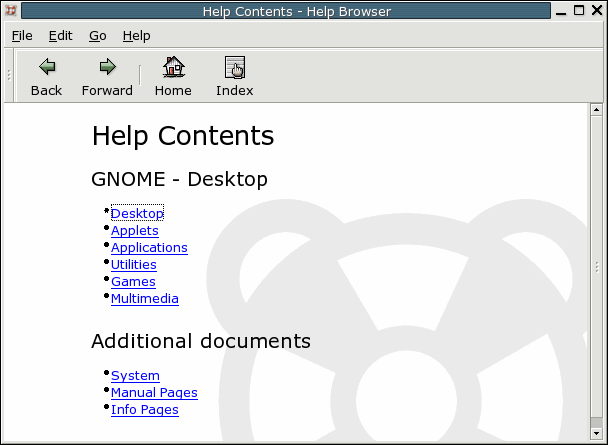
\includegraphics{yelp01.eps}~~~~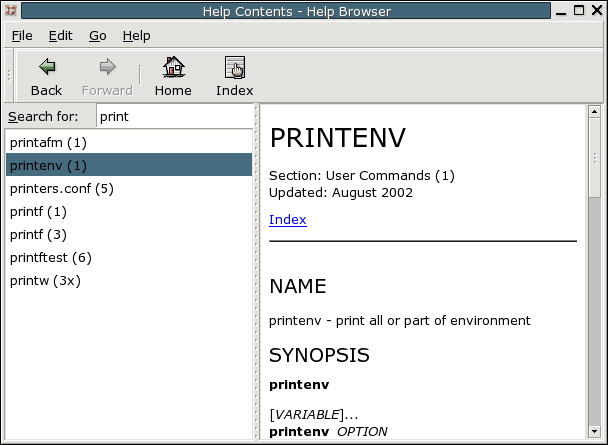
\includegraphics{yelp02.eps}}\caption{GNOME Help browser}\label{fig:yelp}}}%
{\leftskip=\moveback\parbox{\headwidth}{\center\scalebox{.35}{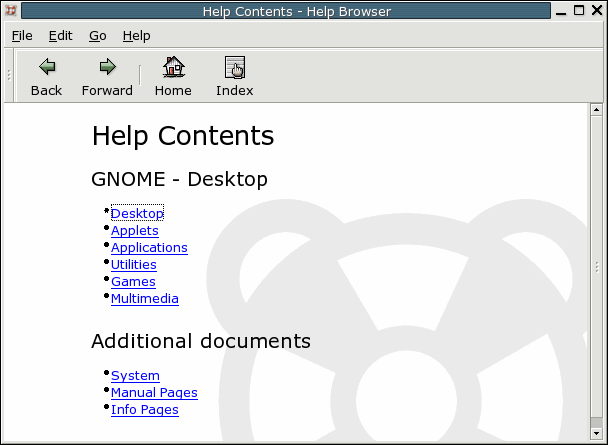
\includegraphics{yelp01.eps}~~~~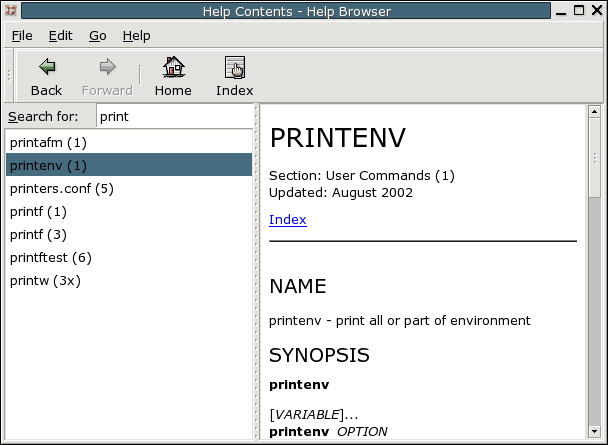
\includegraphics{yelp02.eps}}\caption{GNOME Help browser}\label{fig:yelp}}}
\end{figure}

\begin{figure}[t]
\ifthenelse{\isodd{\pageref{fig:khelpcenter}}}%
{\parbox{\headwidth}{\center\scalebox{.32}{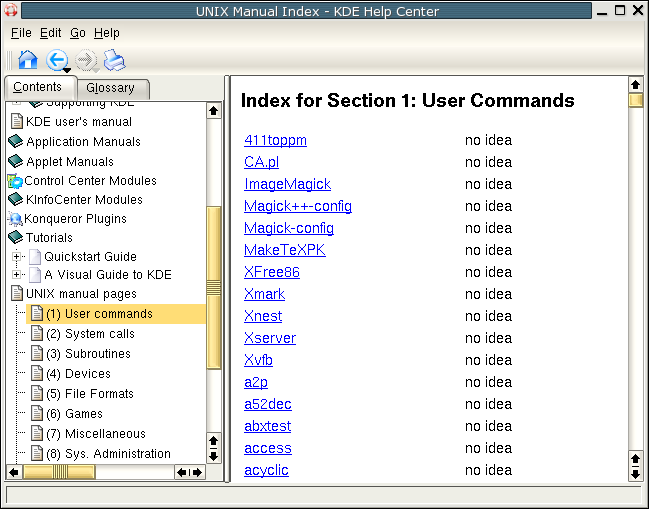
\includegraphics{khelpcenter01.eps}~~~~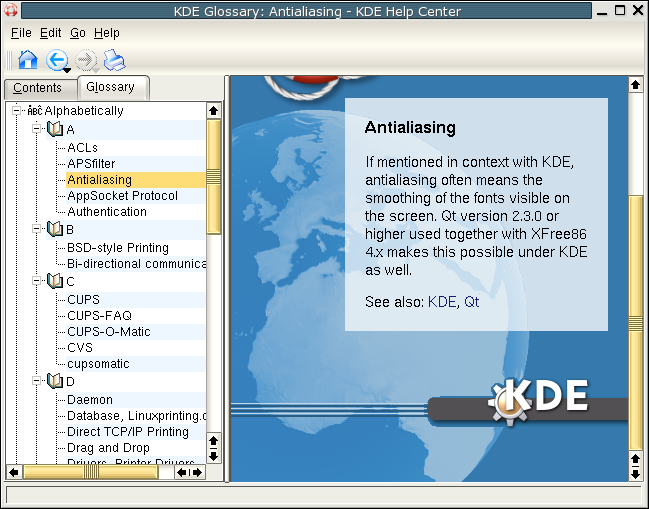
\includegraphics{khelpcenter02.eps}}\caption{KDE Help center}\label{fig:khelpcenter}}}%
{\leftskip=\moveback\parbox{\headwidth}{\center\scalebox{.32}{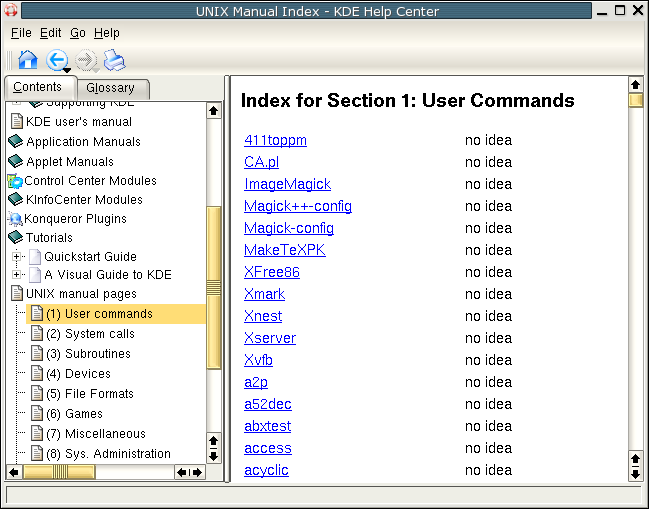
\includegraphics{khelpcenter01.eps}~~~~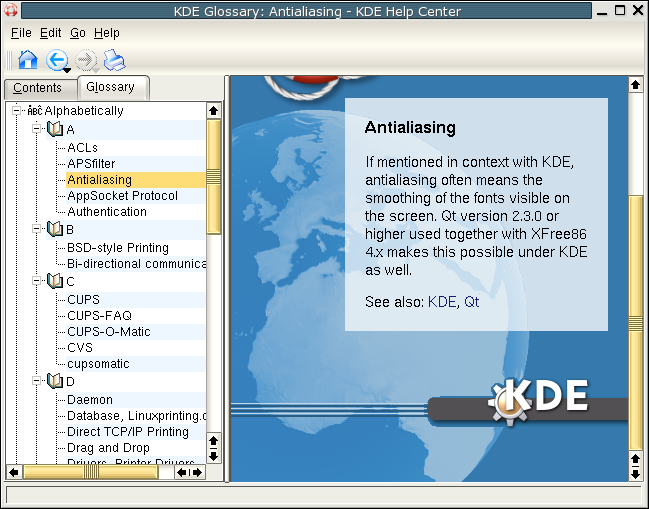
\includegraphics{khelpcenter02.eps}}\caption{KDE Help center}\label{fig:khelpcenter}}}
\end{figure}


\subsubsection{Help ของ bash เชลล์}
จากช่วงที่ผ่านมาเรารู้แล้วว่าคำสั่งที่สั่งในเชลล์พรอมต์มีทั้งคำสั่งภายในซึ่งเชลล์รับรู้กระทำการเองได้และคำสั่งภายนอกซึ่งได้แก่การเรียกโปรแกรมมาใช้งาน. คู่มือการใช้คำสั่งภายในของเชลล์สามารถอ่านได้ด้วยคำสั่ง ``\cmd{man bash}'' หรือ ``\cmd{info bash}''. คู่มือการใช้ \cmd{bash} มีเนื้อหาดี, ผู้ใช้ใหม่ควรจะอ่านคู่มือนี้หนึ่งรอบ.

นอกจากการใช้ \cmd{man} หรือ \cmd{info} แล้ว, bash เชลล์มีคำสั่ง \cmd{help}\cindex{help}\refcmd{help} แสดงวิธีใช้คำสั่งและคำอธิบายอย่างง่ายๆเมื่อให้ชื่อคำสั่งเป็นอาร์กิวเมนต์. ถ้าสั่งคำสั่ง \cmd{help} เดี่ยวๆจะแสดงรายชื่อคำสั่งที่สามารถอธิบายได้.  ตัวอย่างเช่น

\begin{MyExample}[การใช้ \cmd{help} อธิบายคำสั่งภายในของเชลล์]
\begin{MyEx}
$ \cin{help cd}
cd: cd [-L|-P] [dir]
    Change the current directory to DIR.  The variable $HOME is the
    default DIR.  The variable CDPATH defines the search path for
    the directory containing DIR.  Alternative directory names in CDPATH
    are separated by a colon (:).  A null directory name is the same as
    the current directory, i.e. `.'.  If DIR begins with a slash (/),
    then CDPATH is not used.  If the directory is not found, and the
    shell option `cdable_vars' is set, then try the word as a variable
    name.  If that variable has a value, then cd to the value of that
    variable.  The -P option says to use the physical directory structure
    instead of following symbolic links; the -L option forces symbolic 
    links to be followed.
\end{MyEx}
\end{MyExample}

ถ้าคำอธิบายยาวเกินหนึ่งหน้าจอ, เราอาจจะใช้ \cmd{less}\mymemo{ดูสรุปการใช้ \cmd{less} ที่หน้า \pageref{tab:lesskey}.} ช่วยในการแสดงผล.

\begin{MyExample}[การใช้ \cmd{help} ร่วมกับ \cmd{less}.]
\begin{MyEx}
$ \cin{help set | less}
\end{MyEx}
\end{MyExample}

\subsection{เอกสารกำกับโปรแกรมใช้งาน}
เวลาติดตั้งโปรแกรมต่างๆจะมีเอกสารนอกเหนือจาก man page มาด้วย. เอกสารเหล่านี้อาจจะเป็นเอกสารแนะนำโปรแกรม, หนังสืออนุญาติ, ข้อมูลเพิ่มเติม ฯลฯ อยู่ที่ \cmd{/usr/share/doc}. บางครั้งอาจจะมีเอกสารการใช้งานแบบ HTML\myvocab{h}{HTML (Hyper Text Markup Language)}{มาตรฐานสำหรับเขียนเอกสารที่เผยแพร่ทาง World Wide Web. รูปแบบของไฟล์เป็นเนื้อหาเท็กซ์ที่มนุษย์อ่านแล้วเข้าใจได้. ใช้การเขียนกำกับส่วนที่เป็นหัวข้อ, เนื้อหา, รูปภาพ ฯลฯ. โดยปรกติจะใช้เว็บบราวเซอร์ (web browser) ดูไฟล์ HTML. เว็บบราวเซอร์จะทำหน้าที่จัดหน้าจอภาพตามที่เขียนกำกับไว้ในไฟล์.} ใต้ไดเรกทอรีนั้นๆด้วย. ถ้าเป็นเอกสารแบบ HTML ก็ใช้\emph{บราวเซอร์ (browser)} เช่น \cmd{mozilla}, \cmd{konqueror} เปิดอ่านใน X วินโดว์ได้. หรือถ้าต้องการอ่านในเทอร์มินอลก็ใช้บราวเซอร์แบบเท็กซ์โหมดเช่น \cmd{lynx} หรือ \cmd{w3m}.\mymemo{\cmd{w3m} จะมี key binding ทั้งแบบ \cmd{vi} และ \cmd{emacs} ให้ใช้ด้วย. จะให้ความรู้สึกเหมือนกับใช้เพจเจอร์ \cmd{less} แต่เป็นบราวเซอร์. จริงๆแล้ว \cmd{w3m} สามารถใช้เป็นเพจเจอร์ได้ด้วย.}

\subsection{ข้อมูลทางอินเทอร์เน็ต}
\subsubsection{เว็บไซด์อย่างเป็นทางการของดิสทริบิวชันต่างๆ}
ดิสทริบิวชันชั้นนำต่างๆมักจะมีเว็บไซด์เผยแพร่เอกสารที่เกี่ยวกับดิสทริบิวชันเช่น คู่มือการติดตั้ง (Installation Guide), คู่มือเริ่มต้นใช้งาน (User's Guide), คู่มือสำหรับผู้ดูแลระบบ (System Administrator's Manual) ฯลฯ. ผู้ที่สนใจสามารถไปที่เว็บไซด์ของดิสทริบิวชันที่ใช้อยู่และหาเอกสารที่ต้องการ.

นอกจากเว็บไซด์ของดิสทริบิวชันแล้วยังมีเว็บไซด์ The Linux Document Project (TLDP)\cite{tldp} ที่รวบรวมเอกสารต่างๆที่เรียกว่า HOWTO, Guide, FAQ\myvocab{f}{FAQ (Frequently Asked Questions}{การรวมคำถามและคำตอบที่ถามกันบ่อยสรุปไว้เพื่อเป็นข้อมูลสำหรับคนอื่นที่มีคำถามเดียวกัน.} ฯลฯ. เอกสารที่เผยแพร่และรวบรวมโดย TLDP นี้ไม่ขึ้นกับดิสทริบิวชันใดๆและเขียนโดยอาสาสมัครทั่วโลก. เอกสารหลักเป็นภาษาอังกฤษและมีการแปลเป็นภาษาอื่นๆด้วย. เอกสาร HOWTO เป็นเอกสารที่เจาะจงรายละเอียดตั้งแต่เรื่องทั่วๆไปจนถึงเรื่องเฉพาะด้านเช่น วิธีการเซ็ตเชลล์พรอมต์, การสร้าง VPN\myvocab{v}{VPN (Virtual Private Network)}{การใช้เครือข่ายสาธารณะเช่นอินเทอร์เน็ตในการรับส่งข้อมูลโดยมีวิธีการรักษาความปลอดภัยของข้อมูลด้วย. พูดง่ายๆคือการสร้างเครือข่ายที่มีความปลอดภัยสูง (เช่นการลงรหัส) บนเครือข่ายสาธารณะ.} ฯลฯ. เอกสารอีกประเภทที่น่าอ่านของ TLDP อีกประเภทได้แก่เอกสารยาวที่เป็นหนังสือเรียกว่า Guide ต่างๆเช่น Advanced Bash-Scripting Guide, The Linux System Administrators' Guide เป็นต้น. เอกสารเหล่านี้เผยแพร่หลายฟอร์แมตเช่น HTML, PDF, PostScript ฯลฯ. 


แหล่งข้อมูลที่มีประโยชน์อีกแห่งได้แก่เว็บไซด์บริการหาข้อมูลเช่น Google, Yahoo ฯลฯ. หากผู้ใช้มีปัญหาการใช้โปรแกรมเช่นเกิด error ขึ้นตอนใช้งาน, ก็สามารถนำข้อความ error นั้นไปค้นหาบนอินเทอร์เน็ตได้. นอกจากค้นหาจากเว็บไซด์แล้ว, การหาข้อมูลจากนิวส์กรุปเช่นจาก \url{http://groups.google.com} ในบางครั้งจะได้ข้อมูลที่ไม่มีในเว็บก็ได้. 

แหล่งข้อมูลอื่นๆที่ผู้ใช้อาจจะถามคำถามได้เช่นเว็บบอร์ด, ฟอรัม (forum), mailing list เป็นต้น. เว็บไซด์ภาษาไทยที่ผู้อ่านสามารถถามตอบปัญหาต่างๆได้แสดงไว้ในตารางที่ \ref{tab:forums}.

\myvocab{u}{URL (Uniform Resource Locator)}{วิธีการอ้างอิงแหล่งข้อมูลเช่นเอกสารทางอินเทอร์เน็ต. ตัวอย่างเช่น http://linux.thai.net:80/plone ประกอบด้วยส่วนต่างๆได้แก่ โปรโตคอล (http), ชื่อโดเมน (linux.thai.net), หมายเลขพอร์ต (80) และ path (plone).}
\begin{table}[!htb]
\caption{เว็บไซด์ที่บุคคลถามตอบปัญหาได้.}\label{tab:forums}
\bigskip
\begin{tabular}{l|p{.6\textwidth}}
\hline
\multicolumn{1}{c|}{เว็บไซด์} & \multicolumn{1}{|c}{URL}\\
\hline
Thai Linux Working Group & \url{http://linux.thai.net}\\
Linux Siam & \url{http://www.linuxsiam.com}\\
Thai Linux Cafe & \url{http://thailinuxcafe.com}\\
Tux Crazy & \url{http://www.tuxcrazy.com}\\
Grandlinux Solution & \url{http://www.grandlinux.com}\\
\hline
\end{tabular}
\end{table}



\section{การปรับแต่งเชลล์}
โดยปรกติแล้วลินุกซ์ดิสทริบิวชันที่ผู้อ่านติดตั้งนั้นมักจะปรับแต่งเชลล์ไว้ให้เรียบร้อยแล้ว. บ้างก็ตั้งค่าตัวแปรสภาพแวดล้อมที่จำเป็นต่างๆไว้ให้, บ้างก็ปรับแต่งพรอมต์ให้ดูสวยงามใช้ง่าย, บ้างก็สร้าง alias ไว้ให้ ฯลฯ. ในช่วงนี้เราจะมาดูวิธีการปรับแต่งเชลล์เพื่อให้การใช้งานเชลล์สะดวกขึ้น. และเรียนรู้เกี่ยวกับระบบให้ลึกซึ้งยิ่งขึ้น.

\subsection{ไฟล์ตั้งค่าเริ่มต้น}
\mymemo{ในที่นี้จะครอบคลุมเนื้อหาของ bash เท่านั้น.}จากตัวอย่างการสร้าง alias (หน้า \pageref{sec:alias}) ที่ผ่านมา, alias ที่สร้างนั้นจะใช้ได้ในเชลล์ที่ทำงานอยู่เท่านั้น. ถ้าเราจบการใช้งานเชลล์แล้ว alias ที่เราสร้างหรือสิ่งที่เราปรับค่าไว้ก็จะหายไป. ในระบบยูนิกซ์, มักจะมี\emph{ไฟล์ตั้งค่าเริ่มต้น (initialization file)}\gindex{initialization file}\mymemo{ในภาษาอังกฤษ, บ้างก็เรียกไฟล์ตั้งค่าเริ่มต้นว่า init file, rc file\gindex{rc file} หรือ dot file\gindex{dot file}. ไฟล์ตั้งค่าเริ่มต้นมักจะเป็นไฟล์ที่นำหน้าด้วยจุด (\cmd{.}) ทำให้เวลาสั่งคำสั่ง \cmd{ls} แล้วมองไม่เห็น, จึงเรียกว่า dot file. บางทีมีการตั้งชื่อให้ชัดเจนเช่น \cmd{.bashrc} โดยการเติม ``rc''. จากการบอกเล่ากันมา, ``rc'' ย่อมาจาก run command. กล่าวคือเป็นไฟล์ที่เขียนคำสั่งที่ต้องการทำไว้เฉพาะเวลาโปรแกรมนั้นๆเริ่มทำงาน.} ซึ่งเป็นเท็กซ์ไฟล์ที่อ่านได้, ใช้สำหรับเขียนคำสั่งเริ่มต้น, ปรับแต่งค่าตัวแปร, ปรับแต่งพฤติกรรมของโปรแกรม. เชลล์ก็เช่นกันมีไฟล์ตั้งค่าเริ่มต้นของระบบ (system wide) และส่วนบุคคล.

ไฟล์ที่เชลล์อ่านเมื่อเพื่อตั้งค่าเริ่มต้นของระบบนั้นจะแตกต่างกันขึ้นอยู่กับประเภทของเชลล์ที่ใช้ว่าเป็นล็อกอินเชลล์หรือเชลล์เชิงโต้ตอบ. ในกรณีที่เป็นล็อกอินเชลล์, เชลล์จะอ่านค่าเริ่มต้นจากไฟล์ \cmd{/etc/profile} ซึ่งเป็นไฟล์ตั้งค่าเริ่มต้นของระบบก่อน. หลังจากนั้นจะตรวจดูว่าในโฮมไดเรกทอรีมีไฟล์ \cmd{.bash\_profile} หรือ \cmd{.bash\_login} หรือ \cmd{.profile} หรือไม่ตามลำดับ. ถ้ามีเจอไฟล์ใดไฟล์หนึ่งที่กล่าวไปแล้วก็จะอ่านเนื้อหาจากไฟล์นั้นและเลิกค้นหาไฟล์อื่นๆ. ถ้ามีไฟล์ \cmd{.bash\_logout} ในโฮมไดเรกทอรี, เชลล์จะอ่านไฟล์นี้ตอนที่เลิกการทำงาน. 

ในกรณีที่เป็นเชลล์เชิงโต้ตอบเช่น เชลล์ที่อยู่ใน \cmd{xterm}\mymemo{เชลล์ที่ใช้ในเทอร์มินอลเอมิวเลเตอร์บางชนิดเช่น \cmd{gnome-terminal} สามารถเลือกได้ว่าจะใช้ล็อกอินเชลล์หรือเชลล์เชิงโต้ตอบ.} เวลาเริ่มต้นจะอ่านค่าเริ่มต้นในไฟล์ \cmd{.bashrc} ที่อยู่ในโฮมไดเรกทอรีเท่านั้น. 

\begin{figure}[!htb]
\plfigure{.8}{login_logout.eps}{ไฟล์ตั้งค่าเริ่มต้นของ \cmd{bash}}{login_logout}
\end{figure}

เนื่องจากการใช้เชลล์ประเภทต่างกันจะอ่านไฟล์ตั้งค่าเริ่มต้นที่แตกต่างกันไปด้วย.
ดังนั้นถ้าจะตั้งค่าหรือปรับแต่งเชลล์ควรจะระวังด้วยว่าเชลล์ที่กำลังใช้อยู่นั้นอ่านไฟล์ตั้งค่าเริ่มต้นจากที่ไหน.
ลินุกซ์ดิสทริบิวชันบางค่ายปรับแต่งไฟล์เช่น \cmd{.bash\_profile} ให้เชลล์อ่านไฟล์
\cmd{.bashrc} อีกต่อด้วย. หมายความว่าไม่ว่าผู้ใช้จะใช้ล็อกอินเชลล์หรือเชลล์เชิงโต้ตอบ,
การปรับแต่งเชลล์ที่เขียนไว้ในไฟล์จะถูกอ่านเสมอ. 

\subsection{ไฟล์ \cmd{/etc/profile}}
หลังจากที่แนะนำการใช้เชลล์และคำสั่งต่างๆไปพอสมควรแล้ว, เราลองมาดูตัวอย่างไฟล์ตั้งค่าเริ่มต้นเชลล์ \cmd{/etc/profile} ที่ใช้ในลินุกซ์ดิสทริบิวชัน Gentoo กัน. เนื้อหาของไฟล์นี้จะแตกต่างกันตามดิสทริบิวชันค่ายต่างๆแต่ก็มีหน้าที่เหมือนกันคือปรับแต่งค่าเริ่มต้นของล็อกอินเชลล์ในระบบ. ไฟล์นี้เป็นไฟล์ที่มีอยู่แล้วไม่ต้องเขียนเองและไม่ควรแก้ไขถ้าไม่มีความรู้เกี่ยวกับเชลล์อย่างเพียงพอเพราะไฟล์นี้จะมีผลกระทบกับทุกคนในระบบ. ถ้าต้องการปรับแต่งค่าเริ่มต้นเชลล์เฉพาะบุคคลให้แก้ไฟล์ \cmd{\$HOME/.bash\_profile}.
\mymemo{เครื่องหมาย\raisebox{8pt}{\wrap{}} ใช้แสดงว่าเนื้อหาที่เขียนยังอยู่ในบรรทัดเดียวกันแต่ขึ้นบรรทัดใหม่ให้อ่านง่ายขึ้นเท่านั้น.}

\begin{MyExample}[ไฟล์ตั้งค่าเริ่มต้นของเชลล์]\label{ex:profile}
\begin{MyEx}
$ \cin{cat -n /etc/profile}
     1  # /etc/profile:
     2  # $Header: /home/cvsroot/gentoo-src/rc-scripts/etc/profile,v\wrap
1.23 2003/04/29 21:23:18 azarah Exp $ 
     3
     4  if [ -e "/etc/profile.env" ]
     5  then
     6          . /etc/profile.env
     7  fi
     8
     9  # 077 would be more secure, but 022 is generally quite realistic
    10  umask 022
    11
    12  if [ `/usr/bin/whoami` = 'root' ]
    13  then
    14          # Do not set PS1 for dumb terminals
    15          if [ "$TERM" != 'dumb'  ] && [ -n "$BASH" ]
    16          then
    17                  export PS1='\bs{}[\bs{}033[01;31m\bs{}]\bs{}h \bs{}[\bs{}033[01;34m\bs{}]\bs{}W \wrap
\bs{}$ \bs{}[\bs{}033[00m\bs{}]'
    18          fi
    19          export PATH="/bin:/sbin:/usr/bin:/usr/sbin:${ROOTPATH}"
    20  else
    21          # Do not set PS1 for dumb terminals
    22          if [ "$TERM" != 'dumb'  ] && [ -n "$BASH" ]
    23          then
    24                  export PS1='\bs{}[\bs{}033[01;32m\bs{}]\bs{}u@\bs{}h \bs{}[\bs{}033[01;34m\bs{}]\wrap
\bs{}W \bs{}$ \bs{}[\bs{}033[00m\bs{}]'
    25          fi
    26          export PATH="/bin:/usr/bin:${PATH}"
    27  fi
    28  unset ROOTPATH
    29
    30  if [ -z "$INPUTRC" -a ! -f "$HOME/.inputrc" ]
    31  then
    32          export INPUTRC="/etc/inputrc"
    33  fi
    34
    35  # Extract the value of EDITOR
    36  [ -z "$EDITOR" ] && EDITOR="`. /etc/rc.conf 2>/dev/null; \wrap
echo $EDITOR`"
    37  [ -z "$EDITOR" ] && EDITOR="`. /etc/conf.d/basic 2>/dev/null; \wrap
echo $EDITOR`"
    38  [ -z "$EDITOR" ] && EDITOR="/bin/nano"
    39  export EDITOR
\end{MyEx}
\end{MyExample}
%$

\subsubsection{คอมเมนต์}
บรรทัดที่ 1 และ 2 ขึ้นต้นบรรทัดด้วยเครื่องหมาย number (\cmd{\#}) ซึ่งเชลล์จะไม่แปลความสิ่งที่เขียนหลังเครื่องหมาย number จนสุดบรรทัด. สองบรรทัดแรกนี้เรียกว่า\emph{คอมเมนต์ (comment)}\mymemo{คำว่า comment แปลเป็นภาษาไทยตรงๆได้ว่า ``หมายเหตุ''. แต่ในที่นี้จะใช้ทับศัพท์ว่าคอมเมนต์.} ใช้เขียนอธิบายเนื้อหาที่อยู่ในไฟล์นี้. 

\subsubsection{ตรวจสอบไฟล์ด้วย \cmd{if}}
บรรทัดที่ 4 ถึง 7 เป็นการตรวจสอบว่ามีไฟล์ \cmd{/etc/profile.env} หรือไม่ด้วยคำสั่ง \cmd{if}.\cindex{if}\myexplanation{if}{เป็นคำสั่งผสมที่ใช้ในเชลล์เพื่อตรวจสอบกรณีต่างๆ.}
\begin{MyVerbatim}
if \textit{COMMAND}\mycomment{ถ้าสถานะการจบคำสั่งเป็น 0 จะถือว่าเป็นจริง}
then
    \textit{COMMAND}\mycomment{คำสั่งที่ใช้ในกรณีที่เป็นจริง}
    ...
elif \textit{COMMAND}\mycomment{ตรวจสอบด้วย if อีกครั้ง}
then
    \textit{COMMAND}
    ...
else
    \textit{COMMAND}\mycomment{คำสั่งที่ใช้ในกรณีอื่นๆ (เท็จ)}
    ...
fi\mycomment{จบการตรวจสอบด้วย if}
\end{MyVerbatim}
ให้สังเกตว่าสิ่งที่พิมพ์หลังคำสั่ง \cmd{if} เป็นคำสั่งและคำสั่งนี้จะถูกกระทำการจริง. ถ้าคำสั่งจบบริบูรณ์โดยไม่มีข้อผิดพลาด (สถานะการจบเป็น 0) ก็จะถือว่าการตรวจสอบเป็นจริง. จะกระทำการคำสั่งที่อยู่ในช่วง \cmd{then} ต่อไป. บรรทัดที่ 4 คำสั่งที่ใช้ในการตรวจสอบคือคำสั่ง \cmd{[}\cindex{[} ซึ่งเป็นคำสั่งภายในและเหมือนกับคำสั่ง \cmd{test} (หน้า \pageref{cmd:test}). คำสั่ง \cmd{[} ต้องการอาร์กิวเมนต์ตัวสุดท้ายเป็น \cmd{]} เสมอเพื่อให้ดูเรียบร้อยเหมือนกับไวยกรณ์ของโปรแกรม. กล่าวคือ ``\cmd{[ -e \dq/etc/profile.env\dq ]}''\mymemo{ให้สังเกตว่าหลัง \cmd{[} และก่อนหน้า \cmd{]} ต้องมีช่องไฟเพราะ \cmd{[} เป็นคำสั่งและ \cmd{]} เป็นอาร์กิวเมนต์ของคำสั่ง.} เขียนได้อีกแบบคือ ``\cmd{test -e \dq/etc/profile.env\dq}''. 

\subsubsection{อ่านเนื้อหาไฟล์อื่นเข้ามาในเชลล์}
ถ้ามีไฟล์ \cmd{/etc/profile.env}\mymemo{ในไฟล์ \cmd{/etc/profile.env} มีการประกาศค่าตัวแปรสภาพแวดล้อมต่างๆที่ Gentoo ตั้งค่าไว้.} อยู่ให้เชลล์อ่านเนื้อหาคำสั่งที่อยู่ในไฟล์นั้น. เครื่องหมายจุด (\cmd{.}) ในบรรทัดที่ 6 ก็เป็นคำสั่งภายเชลล์อย่างหนึ่งทำหน้าที่อ่านคำสั่งที่อยู่ในไฟล์ที่เป็นอาร์กิวเมนต์. เมื่อใช้คำสั่ง \cmd{.} กับไฟล์ที่เป็นอาร์กิวเมนต์ก็เหมือนกับการนำคำสั่งที่เขียนอยู่ในไฟล์นั้นมากระทำการในเชลล์ที่ใช้อยู่. คำสั่ง \cmd{.}\cindex{.} ดูผิวเผนดูไม่เหมือนกับเป็นคำสั่ง, จึงมีคำสั่งที่อ่านแล้วเข้าใจคือ \cmd{source}\cindex{source} ซึ่งเป็นคำสั่งที่ทำหน้าที่เหมือนกับ \cmd{.} ทุกประการ.\refcmd{source}

\bigskip
บรรทัดที่ 10 เป็นการตั้งค่าสิทธิ์การใช้ไฟล์โดยใช้คำสั่งภายในเชลล์ \cmd{umask}. จะอธิบายคำสั่งนี้ในช่วงที่แนะนำเรื่องสิทธิ์การใช้ไฟล์. 

\subsubsection{ตั้งค่าพรอมต์}
\begin{table}[!htbp]
\center
\caption{escape sequence ที่ใช้กับเชลล์พรอมต์}\label{tab:shellprompt}
\bigskip
\begin{tabular}{l|p{.7\textwidth}}
\hline
\multicolumn{1}{c|}{escape sequence} & \multicolumn{1}{|c}{ความหมาย}\\
\hline
\cmd{\bs{}a} & อักขระ ASCII กระดิ่ง. จะไม่แสดงอะไรบนหน้าจอแต่จะมีเสียงกระดิ่งออกทางลำโพง.\\
\cmd{\bs{}d} & แสดงวันที่ในพรอมต์ในรูปของ ``วัน เดือน วันที่''.\\
\cmd{\bs{}D\{\textit{FORMAT}\}} &  แสดงวันโดยใช้รูปแบบที่ระบุด้วย \cmdit{FORMAT}. \cmd{strftime(3)} เพิ่มเติมเกี่ยวกับ \cmdit{FORMAT}.\\
\cmd{\bs{}e} & อักขระ ESC.\\
\cmd{\bs{}h} & ชื่อโฮสซึ่งจะแสดงชื่อโฮสถึงเครื่องหมายจุด (\cmd{.}) ที่เจอตัวแรกเท่านั้น. เช่นถ้าชื่อโฮสเป็น \cmd{localhost.localdomain}, \cmd{\bs{}h} ก็จะเป็น \cmd{localhost}.\\
\cmd{\bs{}H} & ชื่อโฮส.\\
\cmd{\bs{}j} & จำนวนจ็อบที่ควบคุมโดยเชลล์นั้น.\\
\cmd{\bs{}l} & basename ของดีไวส์เทอร์มินอลที่ใช้. เช่นเทอร์มินอลที่ใช้คือดีไวส์คือ \cmd{/dev/pst/6}, \cmd{\bs{}l} จะเป็น \cmd{6}.\\
\cmd{\bs{}n} & อักขระ newline ขึ้นบรรทัดใหม่.\\
\cmd{\bs{}r} & อักขระ cariiage return ขึ้นบรรทัดใหม่.\\
\cmd{\bs{}s} & ชื่อเชลล์ที่ใช้.\\
\cmd{\bs{}t} & เวลาปัจจุบันแบบ 24 ชั่วโมงเช่น \cmd{23:59:59}.\\
\cmd{\bs{}T} & เวลาปัจจุบันแบบ 12 ชั่วโมงเช่น \cmd{11:59:59}.\\
\cmd{\bs{}@} & เวลาปัจจุบันแบบ 12 ชั่วโมงเช่น \cmd{11:59 PM}.\\
\cmd{\bs{}A} & เวลาปัจจุบันแบบ 24 ชั่วโมงเช่น \cmd{23:59}.\\
\cmd{\bs{}u} & ชื่อผู้ใช้.\\
\cmd{\bs{}v} & เวอร์ชันของ bash เชลล์ที่ใช้เช่น \cmd{2.00}.\\
\cmd{\bs{}V} & รีลีสของ bash เชลล์ที่ใช้เช่น \cmd{2.00.0} (เวอร์ชัน + patch level).\\
\cmd{\bs{}w} & ไดเรกทอรีที่ทำงานอยู่เช่น \cmd{\~} (โฮมไดเรกทอรี).\\
\cmd{\bs{}W} & ไดเรกทอรีที่ทำงานอยู่เช่น \cmd{somchai} (โฮมไดเรกทอรีของ somchai).\\
\cmd{\bs{}!} & หมายเลขประวัติคำสั่งของคำสั่งนี้.\\
\cmd{\bs{}\#} & หมายเลข (จำนวน) คำสั่ง.\\
\cmd{\bs{}\$} & แสดงพรอมต์ \cmd{\#} ถ้าเป็น root หรือ \cmd{\$} อื่นๆ.\\
\cmd{\bs{}\textit{nnn}} & เลขฐานแปด \cmdit{nnn} ใช้เขียนแทนอักขระที่ไม่สามารพิมพ์ได้.\\
\cmd{\bs\bs} & backslash (\cmd{\bs})\\
\cmd{\bs{}[} & เริ่มอักขระที่แสดงทางหน้าจอไม่ได้ใช้เพื่อพิมพ์อักขระควบคุมเทอร์มินอล.\\
\cmd{\bs{}]} & จบอักขระที่แสดงทางหน้าจอไม่ได้.\\
\hline
\end{tabular}
\end{table}
บรรทัดที่ 12 ถึง 27 เป็นการตั้งค่าพรอมต์และ \cmd{PATH}. จะมีการตรวจสอบว่าถ้าผู้ใช้คือ root ก็จะตั้งค่าพรอมต์และ \cmd{PATH} ให้ต่างจากผู้ใช้ทั่วไป. ตรงนี้มีการใช้ \cmd{test}\refcmd{test} ตรวจสอบผลของคำสั่ง \cmd{whoami}\cindex{whoami}\refcmd{whoami} ว่าได้ผลเป็น root หรือไม่. ก่อนที่จะตั้งค่าพรอมต์มีการตรวจสอบชนิดของเทอร์มินอลว่าไม่ใช่\emph{เทอร์มินอลแบบ dumb (dumb terminal)}.\myvocab{d}{dump terminal}{เป็นเทอร์มินอลโบราณรุ่นแรกๆ. ไม่มีความสามารถในการจัดแต่งหน้าจอ, ไม่มีสี (ขาวดำ) หรือมีขีดจำกัดอื่นๆ. กล่าวคือเป็นเทอร์มินอลแบบง่ายๆ, มีเพียงคุณสมบัติเบื้องต้นที่พอจะใช้งานได้เท่านั้น.} 

ค่าของพรอมต์เก็บอยู่ในตัวแปรสภาพแวดล้อม \cmd{PS1}\gindex{ps1@\cmd{PS1}} ดูซับซ้อนแต่ความจริงไม่ยากที่จะทำความเข้าใจ. พรอมต์ที่ตั้งนี้เป็นพรอมต์ที่มีสีซึ่งใช้คุณสมบัติของ
\emph{เทอร์มินอลมาตรฐาน ANSI (ANSI terminal)}\gindex{ansi termial@ANSI terminal} ในการตกแต่งสีต่างๆ. ค่าของพรอมต์ในบรรทัดที่ 17 และ 24 แบ่งออกได้เป็น 3 ส่วนได้แก่.


\begin{enumerate}
\item escape sequence ของเชลล์\\
escape ของเชลล์จะนำหน้าด้วยเครื่องหมาย backslash (\cmd{\bs}). จากตัวอย่างไฟล์ \cmd{/etc/profile} บรรทัดที่ 17 ได้แก่ \cmd{\bs{}[}, \cmd{\bs{}]}, \cmd{\bs{}h}, \cmd{\bs{}W} และ \cmd{\bs{}@}. ตารางที่ \ref{tab:shellprompt} แสดง escape sequence ที่ใช้ได้และคำอธิบาย.
\item ANSI escape sequence\\
\emph{ANSI escape sequence}\gindex{ansi escape sequence@ANSI!escape sequence} เป็น escape sequence ที่ใช้ควบคุมเทอร์มินอลที่มีคุณสมบัติตามที่ ANSI กำหนด. เทอร์มินอลเอมิวเลเตอร์ที่ใช้ใน X วินโดว์โดยทั่วไปก็จัดอยู่ในพวกนี้. จากบรรทัดที่ 17, ช่วงที่เป็น ANSI escape sequence คือ ``\cmd{\bs{}033[01;31m}''.
\item อักขระทั่วไป\\
อักขระทั่วไปคือเครื่องหมายหรืออักษรที่มองเห็นได้ทางเทอร์มินอลไม่มีความหมายพิเศษสำหรับเชลล์. จากบรรทัดที่ 17 ได้แก่ช่องไฟ. จากบรรทัดที่ 24 ได้แก่เครื่องหมาย \cmd{@}.
\end{enumerate}

\subsubsection{ตั้งค่าตัวแปรสภาพแวดล้อม}
ตั้งแต่บรรทัดที่ 28 จนจบไฟล์เป็นการตั้งค่าตัวแปรสภาพแวดล้อมต่างๆ. บรรทัดที่ 28 จะลบตัวแปรสภาพแวดล้อม \cmd{ROOTPATH} ซึ่งถูกตั้งค่าจากการอ่านไฟล์ \cmd{/etc/profile.env} บรรทัดที่ 6 ด้วยคำสั่ง \cmd{unset}.\cindex{unset}\refcmd{unset} 

บรรทัดที่ 30 ถึง 33 เป็นตั้งค่าตัวแปรสภาพแวดล้อม \cmd{INPUTRC} ซึ่งมีการตรวจก่อนว่าถ้าตัวแปร \cmd{INPUTRC} มีมีความยาวเป็น 0\mymemo{ตัวแปรมีความยาวเป็น 0 หมายถึงไม่มีค่าหรือตัวแปรไม่มีตัวตน.} (\cmd{-z \$INPUTRC})\refcmd{test} และ (\cmd{-a}) ไม่มีไฟล์ \cmd{\$HOME/.inputrc} (\cmd{! -f \$HOME/.inputrc}) จึงจะตั้งค่าตัวแปรสภาพแวดล้อม \cmd{INPUTRC} เป็น \cmd{/etc/inputrc}. ตัวแปรสภาพแวดล้อม \cmd{INPUTRC} เป็นตัวแปรที่เก็บชื่อไฟล์ที่เป็นไฟล์ตั้งค่าเริ่มต้นของ\emph{ไลบรารี readline (readline library)}.\gindex{readline} ไลบรารีนี้ใช้ใน bash เชลล์สำหรับช่วยในการแก้ไขบรรทัดคำสั่ง, การเติมเต็มคำสั่ง. ไฟล์ตั้งค่าเริ่มต้นโดยปริยายจะเป็นไฟล์ \cmd{.inputrc} ที่อยู่ในโฮมไดเรกทอรีของผู้ใช้ดังนั้นจึงมีการตรวจสอบไฟล์นี้ว่ามีอยู่หรือไม่. ถ้าไม่มีตัวระบบก็จะตั้งค่าให้เป็นไฟล์ที่ระบบเตรียมไว้. 

บรรทัดที่ 36 จนจบไฟล์เป็นการตั้งค่าตัวแปรสภาพแวดล้อม \cmd{EDITOR}. ตัวแปร \cmd{EDITOR} จะใช้เมื่อโปรแกรมที่ใช้งานอยู่ต้องการให้ผู้ใช้แก้ไขไฟล์แต่โปรแกรมนั้นไม่ใช่บรรณาธิกรณ์จึงไม่สามารถแก้ไขไฟล์ได้. กรณี่นี้โปรแกรมนั้นจะเรียกบรรณาธิกรณ์ที่ระบุอยู่ในตัวแปรสภาพแวดล้อม \cmd{EDITOR} ขึ้นมาให้ผู้ใช้แก้ไขไฟล์ที่ต้องการ. โปรแกรมที่ทำอย่างนี้เช่น \cmd{less} (เมื่อต้องแก้ไขไฟล์ที่ดูอยู่), \cmd{cvs} (เมื่อต้องการแก้ไขไฟล์หรือเขียนหมายเหตุ) ฯลฯ. 


\subsection{สีที่ใช้ในเทอร์มินอลแบบ ANSI}
ANSI escape sequence เป็น escape sequence ที่ใช้ควบคุมหรือปรับแต่พฤติกรรมของเทอร์มินอลที่มีมาตรฐานแบบ ANSI. escape sequence ที่เกี่ยวกับการปรับแต่งสีมีรูปแบบเป็น
\begin{MyVerbatim}
<ESC>[{\textit{attr1}};...;{\textit{attrn}}m
\end{MyVerbatim}
\begin{itemize}
\item \cmd{<ESC>} คืออักขระ ESC. เนื่องจากอักขระ ESC ไม่สามารถแสดงได้ในเทอร์มินอลได้เลยใช้ \cmd{\bs{}033} ซึ่งเป็นค่าของอักขระ (เลขฐานแปด) แทนในบรรทัดคำสั่ง.

\item \cmd{[} เป็นการเริ่มต้นคุณลักษณะของอักษรที่ต้องการแสดง.
\item ตัวเลขที่ถัดจาก \cmd{[} คือค่าที่ระบุเช่น 01 หมายถึงใช้ตัวหนา. 33 หมายถึงใช้ตัวอักษรสีเหลือง. ในการระบุค่ามากกว่าสองอย่างให้ใช้เครื่องหมาย semi-colon (\cmd{;}) ขั้น.
\item \cmd{m} เป็นการสั่งตั้งค่าที่ระบุ.
\end{itemize}
\mymemo{สี Magenta คือสีที่เกิดจากการผสมแม่สี, สีแดง (Red) และสีฟ้า (Blue). สี Cyan คือสีที่เกิดจากการผสมแม่สี, สีเขียว (Green) และสีฟ้า (Blue).}%

\begin{table}[!htb]
\center
\caption{ANSI escape sequence ที่เกี่ยวกับสี. \cite{ansicolor}}\label{tab:ansiterminal}
\bigskip
\begin{tabular}{l|l}
\hline
\multicolumn{1}{c|}{ค่า} & \multicolumn{1}{|c}{คำอธิบาย}\\
\hline
0 &	ยกเลิกค่าที่ตั้งไว้ทั้งหมด\\
1 &	ทำอักษรที่แสดงให้เข้มขึ้น\\
2 &	ทำอักษรที่แสดงให้จางลง\\
4 &	ขีดเส้นใต้\\
5 &	ทำตัวอักษรให้กระพิบ\\
7 &	สลับเปลี่ยนสีฉากหลังกับสีตัวอักษร\\
8 &	ซ่อนอักษรที่แสดง\\
30 &	ใช้สีตัวอักษรสีดำ (Black)\\	      
31 &	ใช้สีตัวอักษรสีแดง (Red)\\	      
32 &	ใช้สีตัวอักษรสีเขียว (Green)\\      
33 &	ใช้สีตัวอักษรสีเหลือง (Yellow)\\    
34 &	ใช้สีตัวอักษรสีฟ้า (Blue)\\	      
35 &	ใช้สีตัวอักษรสีแดงม่วง (Magenta)\\  
36 &	ใช้สี Cyan\\		      
37 &	ใช้สีตัวอักษรสีขาว (White)\\       
40 &	ใช้ฉากหลังสีตัวอักษรสีดำ (Black)\\	   
41 &	ใช้ฉากหลังสีตัวอักษรสีแดง (Red)\\	   
42 &	ใช้ฉากหลังสีตัวอักษรสีเขียว (Green)\\     
43 &	ใช้ฉากหลังสีตัวอักษรสีเหลือง (Yellow)\\   
44 &	ใช้ฉากหลังสีตัวอักษรสีฟ้า (Blue)\\	   
45 &	ใช้ฉากหลังสีตัวอักษรสีแดงม่วง (Magenta)\\ 
46 &	ใช้ฉากหลังสี Cyan\\		   
47 &	ใช้ฉากหลังสีตัวอักษรสีขาว (White)\\      
\hline
\end{tabular}
\end{table}


การตั้งคุณลักษณะพิเศษของสิ่งที่แสดงบนเทอร์มินอลขึ้นอยู่กับความสามารถของเทอร์มินอลจึงมีการตรวจสอบประเภทของเทอร์มินอลก่อนตั้งค่านี้. เราอาจจะทดลองใช้ \cmd{echo} พิมพ์ ANSI escape sequence ดูทางเทอร์มินอลด้วยตัวเลือก \cmd{-e}.\refcmd{echo}

\begin{MyExample}[การใช้ \cmd{echo} พิมพ์ ANSI escape sequence.]
\begin{MyEx}
\cin{echo -e "\bs{}033[1;4mBold and Underline\bs{}033[0m Normal \bs{}033[1mBold again"}
\underline{\bf{}Bold and Underline} Normal {\bf{}Bold again}
\end{MyEx}
\end{MyExample}

\subsection{เชลล์พรอมต์}
เชลล์พรอมต์ที่ใช้กันทั่วไปมีตั้งแต่แบบง่ายสุดตั้งแต่การใช้เครื่องหมายดอลลาร์ \cmd{\$} จนถึงการใช้สคริปต์และฟอนต์พิเศษช่วย \cite{prompthowto}. พรอมต์ที่ใช้ใน bash มีอยู่ 4 ชนิดเก็บค่าไว้ในตัวแปรสภาพแวดล้อมต่างๆกันได้แก่
\begin{enumerate}
\item \cmd{PS1}\gindex{ps1@\cmd{PS1}}\\
เก็บค่าพรอมต์หลักที่ใช้ในล็อกอินเชลล์หรือเชลล์เชิงโต้ตอบ. เราจะคุ้นเคยกับพรอมต์นี้เพราะเป็นพรอมต์ที่ใกล้ตัวที่สุด. และการปรับแต่งพรอมต์ก็มักจะปรับแต่งค่า \cmd{PS1}. ค่าโดยปริยายของ \cmd{PS1} คือ ``\cmd{\bs{}s-\bs{}v\bs{}\$ }''.\mymemo{หลังเครื่องหมาย \cmd{\$} มีช่องไฟหนึ่งตัว.}
\begin{MyExample}[ค่าปริยายของพรอมต์หลัก \cmd{PS1}.]
\begin{MyEx}
-bash-2.05b$ \cin{echo $PS1}
\bs{}s-\bs{}v$
\end{MyEx}
\end{MyExample}%$
โดยปรกติแล้วดิสทริบิวชันจะปรับแต่งค่า \cmd{PS1} ไว้ให้ในไฟล์ \cmd{/etc/profile}.
\item \cmd{PS2}\gindex{ps2@\cmd{PS2}}\\
เก็บค่าพรอมต์รองใช้แสดงเป็นพรอมต์เมื่อสั่งคำสั่งไม่จบภายในหนึ่งบรรทัดแล้วขึ้นบรรทัดใหม่. ค่าโดยปริยายของพรอมต์รองนี้คือ ``\cmd{> }''.
\begin{MyExample}[ค่าปริยายของพรอมต์รอง \cmd{PS2}.]
\begin{MyEx}
-bash-2.05b$ \cin{"Primary prompt $PS1}
> \cin{Secondary prompt $PS2"}
Primary prompt \bs{}s-\bs{}v$
Secondary prompt >
\end{MyEx}
\end{MyExample}%$
\item \cmd{PS3}\gindex{ps3@\cmd{PS3}}\\
เป็นพรอมต์ที่ใช้กับคำสั่ง \cmd{select}.\cindex{select}\refcmd{select} คำสั่ง \cmd{select} เป็นคำสั่งแบบไวยกรณ์ของเชลล์ที่ใช้แสดงตัวเลือกเป็นข้อๆให้เลือกตอบคำถาม. 
\begin{MyExample}[ใช้ \cmd{select} ถามคำถาม.]
\begin{MyEx}
$ \cin{echo What is your favorite character in One Piece?;\bs{}}
> \cin{select name in Luffy Nami Zoro Sanji Usopp Choper Robin;}
> \cin{do echo I like $name also!}
> \cin{break}
> \cin{done}
What is your favorite character in One Piece?
1) Luffy
2) Nami
3) Zoro
4) Sanji
5) Usopp
6) Choper
7) Robin
#? \cin{6}
I like Choper also!
$ \cin{echo $name}
Chopper
\end{MyEx}
\end{MyExample} 
ถ้าตั้งค่า \cmd{PS3}, คำสั่ง \cmd{select} ก็จะใช้ค่าที่ตั้งไว้เป็นพรอมต์แทน ``\cmd{\#?}''.
\item \cmd{PS4}\gindex{ps4@\cmd{PS4}}\\
เป็นพรอมต์ที่แสดงเมื่อมีการติดตาม (trace) คำสั่ง. การติดตามคำสั่งนี้ทำได้โดยตั้งค่า \cmd{xtrace} หรือรันเชลล์ด้วยตัวเลือก \cmd{-x}. ค่าปริยายของ \cmd{PS4} คือ \cmd{+}.
\begin{MyExample}[การติดตามคำสั่งในเชลล์]\label{ex:shelltrace}
\begin{MyEx}
$ \cin{set -o xtrace} \mycomment{หรือ set -x}
++ echo -ne '\bs{}033]0;somchai@toybox:~\bs{}007'
$ \cin{echo Hello}
+ echo Hello
Hello
++ echo -ne '\bs{}033]0;somchai@toybox:~\bs{}007'
$ \cursorprompt
\end{MyEx}
\end{MyExample}%$
การติดตามคำสั่งในเชลล์มีประโยชน์อย่างยิ่งเมื่อใช้ debug เชลล์สคริปต์ดูการสั่งคำสั่งต่างๆในสคริปต์.
\end{enumerate}

หลังจากที่ได้รู้จักกับพรอมต์ประเภทต่างๆแล้วเราลองมาดูตัวอย่างการตั้งค่าพรอมต์จากสิ่งที่เรียนรู้ไปแล้ว. 
\begin{MyExample}[การปรับค่าพรอมต์จากสิ่งที่เรียนมา.]
\begin{MyEx}
$ \cin{export PS1="-\bs{}[\bs{}033[32m\bs{}d, \bs{}t\bs{}033[0m\bs{}]- [\bs{}w]\bs{}n\bs{}u@\bs{}h \bs{}$  "}
-\textcolor{green}{Tue May 18, 01:38:54}- [~]
somchai@toybox $ \cin{cd /usr/src/linux/Documentation/filesystems}
-\textcolor{green}{Tue May 18, 01:39:04}- [/usr/src/linux/Documentation/filesystems]
somchai@toybox $ \cursorprompt
\end{MyEx}
\end{MyExample}
จากตัวอย่างเป็นการสร้างพรอมต์ให้มีสองบรรทัด. บรรทัดแรกบอกเวลาและไดเรกทอรีที่ทำงานอยู่ (full path). ส่วนบรรทัดที่สองเป็นพรอมต์ธรรมดาบอกชื่อผู้ใช้และชื่อโฮส. สำหรับผู้ที่สนใจเรื่องการตั้งค่าพรอมต์โดยละเอียด, สามารถอ่านได้จากเอกสาร Bash Prompt HOWTO \cite{prompthowto}.


\subsection{ไลบรารี readline}
ตามที่ได้แนะนำไปข้างต้นแล้วว่าเชลล์ใช้ไลบรารี readline ช่วยในการปรับแต่งบรรทัดคำสั่งและจัดการประวัติคำสั่ง. เนื่องจาก readline เป็นไลบรารี, โปรแกรมอื่นๆที่มีการโต้ตอบกับผู้ใช้แบบ CLI ก็สามารถใช้ไลบรารี readline ได้ด้วย. ตัวอย่างเช่นโปรแกรม \cmd{gnuplot}\mymemo{\cmd{gnuplot} เป็นโปรแกรมเขียนกราฟ.} ซึ่งมีอินเทอร์เฟสแบบ CLI ก็สามารถใช้ key binding เหมือนกับที่ใช้กับ bash เชลล์ เช่น \cmd{C-p} สั่งคำสั่งที่สั่งไปแล้ว เป็นต้น.

ไลบรารี readline จะอ่านไฟล์ที่ระบุโดยตัวแปรสภาพแวดล้อม \cmd{INPUTRC} หรือถ้าไม่มีการตั้งค่าตัวแปรนี้ก็จะอ่านค่าเริ่มต้นจากไฟล์ \cmd{\$HOME/.inputrc}\gindex{.inputrc@\cmd{.inputrc}}. เราลองมาดูเนื้อหาของไฟล์ตั้งค่าเริ่มต้นของไลบรารี readline กัน. 
\begin{MyExample}[ไฟล์ตั้งค่าเริ่มต้นของไลบรารี readline.]\label{ex:inputrc}
\begin{MyEx}
$ \cin{cat -n ~/.inputrc}
     1  $include /etc/inputrc
     2
     3  # be quiet
     4  set bell-style none
     5  set meta-flag on
     6  set input-meta on
     7  set convert-meta off
     8  set output-meta on
     9
    10  "\bs{}C-x\bs{}C-r": re-read-init-file			       
    11  "\bs{}M-m": "LANG=ja_JP XMODIFIERS='@xim=kinput2' mozilla &"   
    12  								       
    13	$if gnuplot						       
    14  "\bs{}M-m": "plot sin(x)\bs{}r"				       
    15  $endif                                                         
    16  "\bs{}M-xf": dump-functions
    17  "\bs{}M-xv": dump-variables
    18  "\bs{}M-xm": dump-macros
\end{MyEx}
\end{MyExample}

ก่อนที่จะอธิบายเนื้อหาในไฟล์นี้, เราพอจะสังเกตุได้ว่าคอมเมนต์ของไฟล์นี้คือเครื่องหมาย number (\cmd{\#}) และไวยกรณ์ที่ใช้ในไฟล์นี้แบ่งออกเป็น 3 ชนิดใหญ่ๆคือ
\begin{enumerate}
\item ตั้งค่าตัวแปร\\
การตั้งค่าตัวแปรในไฟล์ \cmd{\~{ }/.inputrc} มีไวยกรณ์เป็น
\begin{MyVerbatim}
set \textit{variable-name} \textit{value}
\end{MyVerbatim}
``\cmd{set \textit{variable-name} \textit{value}}'' ในที่นี้ไม่ใช่คำสั่งเชลล์แต่เป็นไวยกรณ์ของไฟล์ตั้งค่าเริ่มต้น readline, จะนำไปใช้ในเชลล์ไม่ได้. ชื่อตัวแปรที่สำคัญและค่าโดยปริยายที่ใช้ในไฟล์ \cmd{\~{ }/.inputrc} ได้แก่.

\begin{itemize}
\item \cmd{bell-style} (\cmd{audible})\mymemo{ค่าที่อยู่ในวงเล็บคือค่าโดยปริยาย.}\\
รูปแบบของกระดิ่งที่ใช้ในเทอร์มินอล. \cmd{audible} คือใช้เสียงกระดิ่งออกทางลำโพง. ถ้าใช้ค่า \cmd{visible} จะไม่มีเสียงแต่หน้าจอจะกระพิบแทน. ส่วน \cmd{none} คือไม่มีอะไรเกิดขึ้น.
\item \cmd{completion-ignore-case} (\cmd{off})\\
ถ้าตั้งค่าเป็น \cmd{on} จะเติมเต็มคำสั่งหรือชื่อไฟล์โดยที่ไม่แยกแยะอักษรตัวใหญ่และอักษรตัวเล็ก.
\item \cmd{completion-query-items} (\cmd{100})\\
จำนวนที่เป็นขีดแบ่งว่าให้ถามว่าจะแสดงส่วนเติมเต็มหรือไม่ในกรณีที่ส่วนเติมเต็มเกินจำนวนที่ตั้งไว้.
\item \cmd{convert-meta} (\cmd{on})\\
ถ้ามีค่าเป็น \cmd{on}, readline จะแปลงอักขระที่เป็น 8 บิตเป็น 7 บิตโดยบิตที่แปดจะใช้อักขระ ESC เป็นตัวแทน. ขึ้นอยู่กับความสามารถของเทอร์มินอลด้วย.
\item \cmd{disable-completion} (\cmd{off})\\
ถ้าตั้งค่าเป็น \cmd{off} จะไม่มีการเติมเต็มให้.
\item \cmd{editing-mode} (\cmd{emacs})\\
ตั้งค่าวิธีการปรับแต่งบรรทัดคำสั่งแบบ \cmd{emacs} หรือ \cmd{vi}.
\item \cmd{expand-tilde} (\cmd{off})\\
เครื่องหมาย tilde (\cmd{\~{ }}) ใช้แทนโฮมไดเรกทอรี. ถ้าตั้งค่าตัวแปรนี้เป็น \cmd{on}, เวลาเติมเต็มจะกระจายเครื่องหมาย tilde เป็น full path.
\item \cmd{input-meta} (\cmd{off})\\
ถ้าตั้งค่าเป็น \cmd{on}, readline จะอนุญาตให้ข้อมูลเข้าเป็นอักขระ 8 บิต. \cmd{meta-flag} เป็นตัวแปรที่มีหน้าที่เหมือนตัวแปรตัวนี้.
\item \cmd{mark-directories} (\cmd{on})\\
ถ้าค่าเป็น \cmd{on}, เวลาเติมเต็มชื่อไฟล์จะใส่เครื่องหมาย slash (\cmd{/}) หลังชื่อไดเรกทอรีเพื่อแยกแยะระหว่างไฟล์ให้ชัดเจน.
\item \cmd{match-hidden-files} (\cmd{on})\\
readline จะแสดงไฟล์ที่เป็นส่วนเติมเต็มทั้งหมดรวมทั้งไฟล์ที่ขึ้นต้นด้วยจุด (\cmd{.}) ด้วย. ถ้าตั้งค่าเป็น \cmd{off} และต้องการเติมเต็มไฟล์ที่ขึ้นต้นด้วยจุด, ต้องพิมพ์จุดก่อนแล้ว readline จะเติมเต็มไฟล์ที่ขึ้นต้นด้วยจุดให้.
\item \cmd{output-meta} (\cmd{off})\\
ถ้าตั้งค่าเป็น \cmd{on}, readline จะแสดงอักขระแบบ 8 บิตให้โดยที่ไม่พยายามเปลี่ยนเป็น 7 บิต. ขึ้นอยู่กับเทอร์มินอลที่ใช้ด้วย.
\item \cmd{page-completions} (\cmd{on})\\
readline จะใช้เพจเจอร์แบบ \cmd{more} ในการแสดงส่วนเติมเต็มที่มีมากกว่าที่จะแสดงบนหน้าจอเดียวได้. ถ้าตั้งค่าเป็น \cmd{off} และมีส่วนเติมเต็มมากจะทำให้ดูยาก, แต่จะไม่ถูกรบกวนด้วยเพจเจอร์. อาจจะใช้คีย์ \kk{Shift}+\kk{PgUp} ย้อมกลับไปดูส่วนเติมเต็มก็ได้.
\end{itemize}
\item Key bindings\\
key binding ที่ใช้อยู่ในเชลล์เช่น \cmd{C-p}, \cmd{C-k} เหล่านี้กำหนดโดยไลบรารี readline ทั้งนั้น. ไลบรารี readline จะเชื่อมคีย์ที่กำหนดไว้หรือผู้ใช้กำหนดไว้เข้ากับคำสั่งของไลบรารี readline. การกำหนดว่าคีย์ไหนจะให้ทำอะไรมีไวยกรณ์ดังนี้.
\begin{MyVerbatim}
\textit{keys}: \textit{action}
\end{MyVerbatim}

\cmdit{keys} อาจจะเป็นชื่อคีย์ที่ readline ได้กำหนดไว้แล้วได้แก่ \cmd{DEL}, \cmd{ESC}, \cmd{ESCAPE} ฯลฯ. ชื่อคีย์เหล่านี้สามารถอ่านได้จาก on-line manual หรือ info ของ readline. \cmdit{keys} อีกแบบคือชุดคีย์ที่ต้องกดคีย์ \kk{Ctrl} ค้างแล้วตามด้วยคีย์อื่น (\cmd{\bs{}C-}), กดคีย \kk{Esc} ก่อนแล้วตามด้วยคีย์อื่น (\cmd{M-}), หรือ กดคีย์ \kk{Esc} ก่อนแล้วตามด้วยการกดคีย์ \kk{Ctrl} ค้างไว้แล้วตามด้วยคีย์อื่น (\cmd{M-C-}). การกดคีย์เหล่านี้มีอิทธิพลมาจากบรรณาธิกรณ์ Emacs. 

\cmdit{action} เป็นการกระทำที่เกิดจากการกดคีย์ที่กำหนดไว้. การกระทำนี้อาจจะเป็นฟังชันของ readline ตามตัวอย่างบรรทัดที่ 10 เช่นถ้ากดคีย์ \cmd{C-x C-r} แล้ว, การกระทำคือฟังชัน \cmd{re-read-init-file}. readline จะอ่านไฟล์ตั้งค่าเริ่มต้นที่กำหนดโดยตัวแปรสภาพแวดล้อม \cmd{INPUTRC} อีกครั้ง. โดยปรกติฟังชันเหล่านี้จะมี key binding โดยปริยายอยู่แล้ว. ถ้าต้องการใช้คีย์อื่นหรือต้องการระบุให้ชัดเจนก็เขียนลงในไฟล์ตั้งค่าเริ่มต้นได้. ในตารางที่ \ref{tab:readlinefunc}\mymemo{key binding บางตัวได้อธิบายไปแล้วในตารางที่ \ref{tab:controlterm} และ \ref{tab:lineedit}} แสดง key binding โดยปริยายและชื่อฟังชันที่สัมพันธ์กัน.

\begin{table}[!htb]
\center
\caption{key binding โดยปริยายและฟังชันไลบรารี readline ที่สัมพันธ์กัน.}\label{tab:readlinefunc}
\bigskip\scriptsize
\begin{tabular}{|c|l||c|l|}
\hline
\multicolumn{2}{|c||}{key binding แบบ \cmd{C-}} & \multicolumn{2}{|c|}{key binding แบบ \cmd{M-}}\\
\hline
\cmd{C-@} &   \cmd{set-mark}&                                  \cmd{M-C-g} &   \cmd{abort}				       \\
\cmd{C-a} &   \cmd{beginning-of-line}&		                \cmd{M-C-h} &   \cmd{backward-kill-word}		       \\
\cmd{C-b} &   \cmd{backward-char}&		                \cmd{M-C-i} &   \cmd{tab-insert}			       \\
\cmd{C-d} &   \cmd{delete-char}&		                \cmd{M-C-j} &   \cmd{vi-editing-mode}			       \\
\cmd{C-e} &   \cmd{end-of-line}&		                \cmd{M-C-m} &   \cmd{vi-editing-mode}			       \\
\cmd{C-f} &   \cmd{forward-char}&		                \cmd{M-C-r} &   \cmd{revert-line}			       \\
\cmd{C-g} &   \cmd{abort}&			                \cmd{M-C-y} &   \cmd{yank-nth-arg}			       \\
\cmd{C-h} &   \cmd{backward-delete-char}&	                \cmd{M-C-[} &   \cmd{complete}				 \\      
\cmd{C-i} &   \cmd{complete}&			                \cmd{M-C-]} &   \cmd{character-search-backward}		   \\    
\cmd{C-j} &   \cmd{accept-line}&		                \cmd{M-space} &   \cmd{set-mark}			       \\
\cmd{C-k} &   \cmd{kill-line}&			                \cmd{M-\#} &   \cmd{insert-comment}			       \\
\cmd{C-l} &   \cmd{clear-screen}&		                \cmd{M-\&} &   \cmd{tilde-expand}			       \\
\cmd{C-m} &   \cmd{accept-line}&		                \cmd{M-*} &   \cmd{insert-completions}			 \\      
\cmd{C-n} &   \cmd{next-history}&		                \cmd{M--} &   \cmd{digit-argument}			       \\
\cmd{C-p} &   \cmd{previous-history}&		                \cmd{M-.} &   \cmd{yank-last-arg}			       \\
\cmd{C-q} &   \cmd{quoted-insert}&		                \cmd{M-<} &   \cmd{beginning-of-history}		       \\
\cmd{C-r} &   \cmd{reverse-search-history}&	                \cmd{M-=} &   \cmd{possible-completions}		       \\
\cmd{C-s} &   \cmd{forward-search-history}&	                \cmd{M->} &   \cmd{end-of-history}			       \\
\cmd{C-t} &   \cmd{transpose-chars}&		                \cmd{M-?} &   \cmd{possible-completions}		       \\
\cmd{C-u} &   \cmd{unix-line-discard}&		                \cmd{M-b} &   \cmd{backward-word}			       \\
\cmd{C-v} &   \cmd{quoted-insert}&		                \cmd{M-c} &   \cmd{capitalize-word}			       \\
\cmd{C-w} &   \cmd{unix-word-rubout}&		                \cmd{M-d} &   \cmd{kill-word}				       \\
\cmd{C-y} &   \cmd{yank}&			                \cmd{M-d} &   \cmd{forward-word}			       \\
\cmd{C-]} &   \cmd{character-search}&		                \cmd{M-l} &   \cmd{downcase-word}			       \\
\cmd{C-\_} &  \cmd{undo}&			                \cmd{M-n} &   \cmd{non-incremental-forward-search-history}     \\
\cmd{C-?} &       \cmd{backward-delete-char}&	                \cmd{M-p} &   \cmd{non-incremental-reverse-search-history}     \\
\cline{1-2}
\multicolumn{2}{c||}{}                  &                     \cmd{M-r} & \cmd{revert-line}\\
\multicolumn{2}{c||}{}			&	               \cmd{M-t} &  \cmd{transpose-words}			     \\
\multicolumn{2}{c||}{}			&			\cmd{M-u} & \cmd{upcase-word}				       \\
\multicolumn{2}{c||}{}			&                      \cmd{M-y} & \cmd{yank-pop}				 \\      
\multicolumn{2}{c||}{}			&			\cmd{M-\bs{}} & \cmd{delete-horizontal-space}		   \\    
\multicolumn{2}{c||}{}			&			 \cmd{M-\~}  &\cmd{tilde-expand}			     \\  
\multicolumn{2}{c||}{}			&			 \cmd{M-C-?} &  \cmd{backward-kill-word}		       \\
\multicolumn{2}{c||}{}			&			 \cmd{M-\_} &  \cmd{yank-last-arg}                             \\ 
\cline{3-4}
\end{tabular}	
\end{table}	

บรรทัดที่ 16-18 เป็นการกำหนด key binding สำหรับฟังชันพิเศษเช่น แสดงรายการของ key binding (\cmd{M-x f}) และฟังชันทั้งหมดที่ใช้ (\cmd{dump-functions}) เป็นต้น. ฟังชัน dump เหล่านี้โดยปรกติไม่มีการตั้งค่า key binding ไว้โดยปริยายนอกจากจะตั้งค่าเองตามตัวอย่าง. ผู้ใช้สามารถดูผลของ key binding นี้ได้จากตัวอย่างที่ \ref{ex:dump-functions}.
\begin{MyExample}[การใช้ฟังชัน \cmd{dump-functions} ตามที่กำหนดใน \cmd{.inputrc}.]\label{ex:dump-functions}
\begin{MyEx}
$ \kk{Esc} \kk{x} \kk{f}
                                                              
abort can be found on "\bs{}C-g", "\bs{}C-x\bs{}C-g", "\bs{}M-\bs{}C-g".
accept-line can be found on "\bs{}C-j", "\bs{}C-m".
alias-expand-line is not bound to any keys
arrow-key-prefix is not bound to any keys
backward-byte is not bound to any keys
backward-char can be found on "\bs{}C-b", "\bs{}M-[D".
...
\end{MyEx}
\end{MyExample}%$


key binding ยังสามารถใช้เรียก\emph{แมโคร (macro)}\myvocab{m}{macro}{\emph{แมโคร}. ชื่อที่กำหนดไว้และกระจายต่อไปคำอื่นๆต่อไป. แมโครใช้กันอย่างกว้างขวางเช่นในภาษาซี, \LaTeX{} ฯลฯ.} แทนคำหรือประโยคที่เรากำหนดไว้ได้ตามตัวอย่างที่ \ref{ex:inputrc} บรรทัดที่ 11. คำหรือประโยคที่เรากำหนดต้องเขียนอยู่ในเครื่องหมาย double quote (\dq). ตามตัวอย่างถ้ากดคีย์ \cmd{M-m}, คำสั่งที่เขียนเตรียมไว้ซึ่งได้แก่ ``\cmd{LANG=ja\_JP XMODIFIERS='@xim=kinput2' mozilla \&}'' จะแทรกอยู่ในบรรทัดคำสั่งให้เหมือนพิมพ์จากแป้นพิมพ์.


\item เงื่อนไข\\
บรรทัดที่ขึ้นต้นด้วยเครื่องหมายดอลลาร์ (\cmd{\$}) เป็นไวยกรณ์ที่ระบุเงื่อนไขหรือคำสั่งพิเศษ. บรรทัดที่ 1 เป็นการรวมค่าเริ่มต้นจากไฟล์ \cmd{/etc/inputrc} เข้ามาในไฟล์. ส่วนบรรทัดที่ 13 เป็นการระบุเงื่อนไขแยก key binding ตามโปรแกรมที่ใช้. ในตัวอย่างถ้าโปรแกรมที่ใช้คือ \cmd{gnuplot}, \cmd{M-m} จะแทน ``\cmd{plot sin(x)\bs{}r}'' ในบรรทัดคำสั่งให้.

นอกจากจะสร้างเงื่อนไขตามโปรแกรมที่ใช้แล้ว, ยังสามารถสร้างเงื่อนไขแบ่งตาม mode (\cmd{emacs} หรือ \cmd{vi}) และประเภทของเทอร์มินอลได้ด้วย. ให้อ่านรายละเอียดเพิ่มเติมจาก online manual หรือ info ของ readline.
\end{enumerate}


\subsubsection{โปรแกรมนี้ใช้ readline หรือไม่?}
โปรแกรมที่มีอินเทอร์เฟสแบบ CLI เช่น \cmd{bash}, \cmd{wc}, \cmd{gnuplot} ฯลฯ มักจะใช้ไลบรารี readline. ดังนั้นจะตรวจสอบดูว่าโปรแกรมนั้นใช้ไลบรารี readline หรือไม่ก็ลองใช้ key binding เช่น \cmd{C-p}, \cmd{C-b} ฯลฯ หรือมีความสามารถเติมเต็มชื่อไฟล์หรือไม่. ถ้าใช้ได้แสดงว่าโปรแกรมนั้นน่าจะใช้ไลบรารี readline.

วิธีตรวจอีกวิธีหนึ่งคือดูจาก \emph{shared library}\mymemo{บ้างก็เรียก shared library ว่า dynamic library.}\myvocab{s}{shared library}{ไฟล์ไบนารีที่เป็นส่วนของไลบรารี. โปรแกรมที่สร้างไม่ต้องรวมส่วนที่เป็นไลบรารีเข้าไปในตัวโปรแกรม. เรียกอีกอย่างหนึ่งว่า dynamic library.} ที่โปรแกรมนั้นใช้. โดยปรกติโปรแกรมที่ใช้ในลินุกซ์มันเป็นโปรแกรมแบบ dynamic, กล่าวคือจะเรียกรวมภาษาเครื่องกลส่วนที่เป็นไลบรารีเมื่อเรียกใช้. วิธีตรวจสอบว่าโปรแกรมนั้นใช้ shared library อะไรได้ด้วยคำสั่ง \cmd{ldd}.\cindex{ldd}\refcmd{ldd} โปรแกรม \cmd{ldd} เป็นโปรแกรมที่ใช้แสดง shared library ที่โปรแกรมใช้.  
\begin{MyExample}[ใช้ \cmd{ldd} ตรวจสอบ shared library]
\begin{MyEx}
$ \cin{ldd /usr/bin/gnuplot}
        linux-gate.so.1 =>  (0xffffe000)
        lib3dkit.so.1 => /usr/lib/lib3dkit.so.1 (0x40015000)
        libvgagl.so.1 => /usr/lib/libvgagl.so.1 (0x4002a000)
        libplot.so.2 => /usr/lib/libplot.so.2 (0x40038000)
        libreadline.so.4 => /lib/libreadline.so.4 (0x4016b000)
	...
\end{MyEx}
\end{MyExample}%$
จะเห็นว่าผลลัพธ์ของคำสั่ง \cmd{ldd} มีบรรทัด \cmd{libreadline} อยู่หมายความว่าโปรแกรมนั้นใช้ไลบรารี readline.

\subsection{ไฟล์ \cmd{\$HOME/.bash\_profile}}\label{ex:bashprofile}
\begin{MyExample}[เนื้อหาของไฟล์ \cmd{.bash\_profile}]
\begin{MyEx}
     1  # /etc/skel/.bash_profile:
     2  # $Header: /home/cvsroot/gentoo-src/rc-scripts/etc/skel/.bash_profile,v\wrap
1.10 2002/11/18 19:39:22 azarah Exp $
     3
     4  #This file is sourced by bash when you log in interactively.
     5  [ -f ~/.bashrc ] && . ~/.bashrc
\end{MyEx}
\end{MyExample}

ไฟล์ตั้งค่าเริ่มต้นของล็อกอินเชลล์อีกไฟล์หนึ่งได้แก่ไฟล์ \cmd{.bash\_profile}. ในตัวอย่าง \ref{ex:bashprofile} เป็นไฟล์ที่สร้างขึ้นโดยระบบตอนที่สร้างบัญชีผู้ใช้. ถ้ามีสิ่งที่ต้องการทำหรือตั้งค่าพิเศษสำหรับล็อกอินเชลล์เฉพาะบุคคลก็ให้เขียนในไฟล์นี้. ในตัวอย่างไม่มีการปรับแต่งอะไรเป็นพิเศษนอกจากอ่านไฟล์ตั้งค่าเริ่มต้นจากไฟล์ \cmd{.bashrc} เท่านั้น. 

\subsection{ไฟล์ \cmd{\$HOME/.bashrc}}
\begin{MyExample}[เนื้อหาของไฟล์ \cmd{.bashrc}]
\begin{MyEx}
     1  # /etc/skel/.bashrc:
     2  # $Header: /home/cvsroot/gentoo-src/rc-scripts/etc/skel/.bashrc,v \wrap
1.8 2003/02/28 15:45:35 azarah Exp $
     3
     4  # This file is sourced by all *interactive* bash shells on startup.  This
     5  # file *should generate no output* or it will break the scp and rcp commands.
     6
     7  # colors for ls, etc.
     8  eval `dircolors -b /etc/DIR_COLORS`
     9  alias d="ls --color"
    10  alias ls="ls --color=auto -F"
    11  alias ll="ls --color -l"
    12  
    13  alias rm='rm -i'
    14  alias cp='cp -i'
    15  alias mv='mv -i'
    16
    17  # Change the window title of X terminals
    18  case $TERM in
    19          xterm*|rxvt|Eterm|eterm)
    20                  PROMPT_COMMAND='echo -ne "\bs{}033]0;$\{USER\}@$\{HOSTNAME%%.*\}:\wrap
$\{PWD/$HOME/~\}\bs{}007"'
    21                  ;;
    22          screen)
    23                  PROMPT_COMMAND='echo -ne "\bs{}033_$\{USER\}@$\{HOSTNAME%%.*\}:\wrap
$\{PWD/$HOME/~\}\bs{}033\bs{}\bs{}"'
    24                  ;;
    25  esac
\end{MyEx}
\end{MyExample}%$
ไฟล์ \cmd{.bashrc}\gindex{.bashrc@\cmd{.bashrc}} นี้ก็เป็นตัวอย่างไฟล์ที่เอามาจากลินุกซ์ Gentoo เช่นกัน. ไฟล์นี้จะเป็นไฟล์ตั้งค่าเริ่มต้นเชลล์เชิงโต้ตอบ. และเนื่องจากในไฟล์ \cmd{.bash\_profile} มีการระบุให้อ่านไฟล์นี้เข้าไปด้วย, เพราะฉะนั้นค่าทั้งหลายที่ปรับแต่งในไฟล์นี้จะมีผลกับเชลล์ล็อกอินด้วย. การปรับแต่งเชลล์ไฟล์นี้มักจะเป็นการตั้งค่าตัวแปรสภาพแวดล้อมและนามแฝง, ไม่ควรสั่งคำสั่งที่ทำให้เกิดข้อมูลแสดงออกทางหน้าจอ. มิเช่นนั้นจะทำให้ \cmd{scp} และ \cmd{rcp}\mymemo{\cmd{scp} และ \cmd{rcp} เป็นโปรแกรมก็อปปี้ไฟล์ผ่านทางเน็ตเวิร์ก.} ไม่ทำงาน. 

บรรทัดที่ 8 ตั้งให้คำสั่ง \cmd{ls} ใช้สีในการแสดงไฟล์หรือไดเรกทอรี. คำสั่ง \cmd{dircolors}\cindex{dircolors}\refcmd{dircolors} ปรับแต่งสีที่จะใช้กับคำสั่ง \cmd{ls}. คำสั่ง \cmd{dircolors} จะแสดงเนื้อหาการตั้งค่าตัวแปรสภาพแวดล้อม \cmd{LS\_COLORS} ทาง stdout. ตัวแปรสภาพแวดล้อมนี้จะมีผลเมื่อใช้คำสั่ง \cmd{ls} กับตัวเลือก \cmd{--color}. เนื่องจากคำสั่ง \cmd{dircolors} แสดงวิธีการตั้งค่าตัวแปรสภาพแวดล้อมทาง stdout เท่านั้นจึงต้องใช้คำสั่ง \cmd{dircolors} ใน back quote (\cmd{`}) และใช้ \cmd{eval}\cindex{eval}\ref{eval} ตีความกระทำการผลลัพธ์ของ \cmd{dircolors} ให้เชลล์รับรู้. 

บรรทัดที่ 9-15 เป็นการสร้าง alias ของคำสั่งต่างๆ. ในที่นี้มีการสร้าง alias ของคำสั่ง \cmd{ls} ซ้ำตัวเอง (บรรทัดที่ 10). จะเห็นได้ว่ามีการใช้ตัวเลือก \cmd{--color} กับคำสั่ง \cmd{ls} และก่อนหน้านี้ได้ทำการปรับแต่งสีที่ใช้กับคำสั่ง \cmd{ls} ไปแล้ว, ถ้าเราสั่งคำสั่ง \cmd{ls} เดี่ยวๆก็จะแสดงสีแยกตามประเภทของไฟล์ที่แสดงให้ด้วย.

บรรทัดที่ 18-25 เป็นการตั้งค่าตัวแปรสภาพแวดล้อม \cmd{PROMPT\_COMMAND}. ค่าของตัวแปรนี้เป็นคำสั่งที่จะถูกกระทำการทุกครั้งก่อนที่จะแสดงเชลล์พรอมต์. บรรทัดที่ 20 เป็นการตั้งค่า \cmd{PROMPT\_COMMAND} ให้ตั้งชื่อ title bar ของเทอร์มินอลทุกครั้งก่อนที่จะแสดงพรอมต์. การตั้งค่า title bar มีรูปแบบดังนี้.
\begin{MyVerbatim}
echo -ne \dq{}\bs{}033]0;\textit{TITLE}\bs{}007\dq{}
\end{MyVerbatim}

การตั้งชื่อ title bar จะคล้ายกับการปรับแต่งสีที่ใช้ในพรอมต์คือมีการใช้อักขระ ESC (\cmd{\bs{}033}) แต่วลีหลังจากนั้นจะต่างกัน. \cmd{\bs{007}} คืออักขระ BELL ที่เขียนอยู่ในรูปของเลขฐานแปด. ถ้ามีการติดตามคำสั่งในเชลล์เหมือนในตัวอย่างที่ \ref{ex:shelltrace} (หน้า \pageref{ex:shelltrace}) ก็จะเห็นว่ามีการสั่งคำสั่ง \cmd{echo} นี้ก่อนที่จะแสดงเชลล์พรอมต์ทุกครั้ง.



\section{สรุปท้ายบท}
\begin{itemize}
\item ลินุกซ์เป็นระบบปฏิบัติการที่แยกอินเทอร์เฟสอเช่น เชลล์หรือ X วินโดว์ออกจากตัวระบบปฏิบัติการ. อินเทอร์เฟสเหล่านี้เป็นเพียงโปรแกรมตัวกลางที่ใช้ติดต่อระหว่างผู้ใช้กับเคอร์เนล.
\item เชลล์เป็นโปรแกรมแปลคำสั่งและใช้อินเทอร์เฟสที่เรียกว่า CLI (Command Line Interface). คำสั่งในที่นี้แยกออกได้เป็นสองประเภทใหญ่ๆคือ คำสั่งภายใน (build-in command) และคำสั่งภายนอกหรือที่เรียกกันว่าโปรแกรม.
\item เชลล์ bash มีความสามารถในการสร้างนามแฝง (alias), ควบคุมจ็อบ (job), บันทึกประวัติคำสั่ง (history), การเติมเต็มไฟล์หรือคำสั่ง (completion), แก้ไขบรรทัดคำสั่ง (line editing) ฯลฯ. ความสามารถบางอย่างเป็นความสามารถที่เกิดจากการใช้ไลบรารี readline ซึ่งโปรแกรมอื่นๆที่มีอินเทอร์เฟสแบบ CLI บางโปรแกรมก็ใช้ไลบรารีนี้ด้วย. การทำความคุ้นเคยกับไลบรารี readline จะช่วยให้ใช้งานบรรทัดคำสั่งคล่องและสะดวกขึ้น.
\item เชลล์ที่ใช้กันอยู่โดยทั่วไปแบ่งได้เป็น 2 ชนิดใหญ่ได้แก่ เชลล์ล็อกอิน (login shell) และเชลล์เชิงโต้ตอบ (interactive shell). เชลล์ทั้งสองแบบมีไฟล์ตั้งค่าเริ่มต้นที่ต่างกัน. เวลาใช้งานควรจะตระหนักเสมอว่าเชลล์ที่ใช้อยู่เป็นเชลล์ประเภทใด.
\item ข้อมูลที่ประมวลโดยเชลล์มักเป็นข้อมูลแบบเท็กซ์. ผู้ใช้สามารถป้อนผลลัพธ์ของโปรแกรมหนึ่งให้อีกโปรแกรมหนึ่งได้โดยไปป์และบันทึกหรืออ่านข้อมูลจากไฟล์ได้โดยการรีไดเรก.
\item คำสั่งหลักในลินุกซ์มักจะรับข้อมูลจาก stdin (คีย์บอร์ด) ถ้าไม่มีชื่อไฟล์เป็นอาร์กิวเมนต์. และมักจะแสดงผลที่ประมวลออกทาง stdout (หน้าจอ). ถ้าคำสั่งที่ใช้เกิดข้อผิดพลาด, จะแสดงข้อผิดพลาดทาง stderr (หน้าจอ).
\item file descriptor คือตัวเลขจำนวนเต็มที่เฉพาะในแต่ละโปรเซสใช้อ้างอิงไฟล์ที่ใช้งาน. file descriptor ของ stdin, stdout และ stderr ได้แก่ 0, 1 และ 2 ตามลำดับ. เราสามารถใช้ file descriptor เหล่านี้รีไดเรกข้อมูลหาซึ่งกันและกันได้.
\item ลินุกซ์ (ยูนิกซ์ก็เช่นกัน) จะมีโปรแกรมที่เรียกว่ายูทิลิตี้หรือเครื่องมือในการทำงานต่างๆ. โปรแกรมเหล่านี้จะทำงานเฉพาะอย่าง, และทำงานอย่างดี. การแก้ปัญหาที่ไม่อาจใช้โปรแกรมเดียวแก้ได้อาจจะแก้ได้ด้วยการใช้โปรแกรมเล็กๆร่วมกันแก้ปัญหาเช่นใช้ไปป์หรือเชลล์สคริปต์.
\end{itemize}

%\section{คำถามทบทวนความเข้าใจ}
%\begin{description}
%\myprac ให้สังเกตตัวอย่างและตอบคำถามต่อไปนี้
%\begin{MyVerbatim}
%$ unset PATH
%$ ls
%-bash: ls: No such file or directory
%$ cd /etc
%$ ls
%-bash: ls: No such file or directory
%\end{MyVerbatim}
%ทำไมหลังจากที่ลบตัวแปร \cmd{PATH} แล้วบางคำสั่งสามารถใช้ได้, บางคำสั่งไม่สามารถใช้ได้? ถ้าต้องการเซ็ตให้สั่งคำสั่งได้ตามปรกติต้องทำอย่างไร?
%\myprac จากตัวอย่างที่ \ref{ex:psgrep} (หน้า \pageref{ex:psgrep}) ให้สร้างคำสั่งโดยใช้ไปป์ให้ผลลัพธ์ที่ได้เหมือนหรือคล้ายกับคำสั่ง \cmd{pgrep}.
%\myprac จงเปิดหา man page ที่เป็นคำอธิบาย (มาตรฐาน) เกี่ยวกับ regular expression (ไม่ใช่คำสั่ง). 
%\myprac จะรู้ได้อย่างไรว่าเชลล์ที่ใช้อยู่เป็นล็อกอินเชลล์หรือเชลล์เชิงโต้ตอบ.
%\myprac ให้สำรวจว่าในไดเรกทอรี \cmd{/usr/bin} มีโปรแกรมใดบ้างที่ใช้ไลบรารี readline.
%\myprac ให้เติมคำสั่ง ``\cmd{echo This is .bashrc}'' ในท้ายบรรทัดแล้วลองเรียกเชลล์เชิงโต้ตอบดูว่ามีอะไรเกิดขึ้น. หลังจากนั้นให้ใช้ \cmd{scp} จากคอมพิวเตอร์เครื่องอื่นก็อปปี้ไฟล์ผ่านทางเน็ตเวิร์กดูว่ามีอะไรเกิดขึ้น.
%\myprac ให้ผู้อ่านหาวิธีใช้คำสั่ง \cmd{du} แสดงผลเป็น kb (Mega-bytes).
%\myprac ใช้ไปป์ดักจับ stderr ไปเป็น stdin ของโปรแกรมอื่นๆได้หรือไม่? ให้ทดลองด้วยตัวเองดู.
%\myprac จงให้เหตุผลว่าทำไมการรีไดเรกข้อมูลเข้าและออกเป็นไฟล์เดียวกันจึงให้ผลที่ไม่ถูกต้อง.
%\myprac จากตัวอย่างที่ \ref{ex:stdouterr} (หน้า \pageref{ex:stdouterr}) ให้ลองแยก stderr ลงไฟล์อย่างเดียว. ให้ลองเอา stderr มารวมกับ stdout แล้วส่งต่อให้ \cmd{less} ดูผลลัพธ์เป็นหน้าๆ.
%\myprac ให้ตรวจสอบดูว่าคำสั่งที่เราสามารถสั่งได้ในเชลล์พรอมต์มีกี่คำสั่ง (โปรแกรม).
%\myprac ให้คำสั่งหลายๆคำสั่งรวมกันแสดงเนื้อหาของไฟล์ \cmd{/etc/passwd} โดยลำดับแสดงบรรทัดสุดท้ายในไฟล์ก่อนไปเรื่อยๆจนถึงบรรทัดแรก (กลับกับคำสั่ง \cmd{cat}).
%\end{description}


%{\it\latintext ``Many UNIX programs do quite trivial tasks in isolation, but, combined with other programs, become general and usefule tools.''}\\
%{\bf\latintext Brian W.Kernighan and Rob Pike}


%{\it\latintext ``Write programs that do one thing and do it well. Write programs to work together. Write programs that handle text streams, because that is a universal interface.''}\\
%{\bf\latintext Doug McIlroy}




%\vspace{1.5cm}

\end{thwbr}
\wbrin
